\documentclass{beamer}
\usetheme{Madrid}
\usecolortheme{whale}

\usepackage{graphicx}
\usepackage{tikz}
\usetikzlibrary{shapes.geometric, arrows.meta, positioning, calc}
\usepackage{booktabs}
\usepackage{amsmath}
\usepackage{amssymb}
\usepackage{multirow}
\usepackage{array}

\title[Quadrature Down Converter]{Design, Simulation, and Hardware Implementation of a Quadrature Down Converter}
\subtitle{Comprehensive Project Report \& Laboratory Verification Presentation}

\author[Katta, Lakshmi, Kushwanth]{Katta Sri Kaushik \and Lakshmi Sai Bhargav V \and Kushwanth Lanka}

\institute[IIIT Hyderabad]{Department of Electrical and Computer Engineering \\ Center for VLSI and Embedded Systems Technology (CVEST) \\ International Institute of Information Technology, Hyderabad}
\date{May 2026}

\begin{document}

% Slide 1: Title Slide
\begin{frame}
  \titlepage
\end{frame}

% Slide 2: Presentation Outline
\begin{frame}{Presentation Outline}
  \tableofcontents
\end{frame}

\section{System Specifications \& Utility of Quadrature Operation}

% Slide 3: System Specifications & Design Constraints
\begin{frame}{System Specifications \& Design Constraints}
  \begin{block}{Project Performance Requirements \& Directives}
    \begin{itemize}
      \item \textbf{Technology Node \& Models:} TSMC 180nm CMOS technology for NMOS switches and UA741 operational amplifiers.
      \item \textbf{MOSFET Parasitic Modeling:} Geometric layout parameter optimization: $W, L, A_S, A_D, P_S, P_D$.
      \item \textbf{Amplifier Architecture Choice:} Implemented a discrete \textbf{CE BJT Amplifier} stage with emitter degeneration for low-distortion output voltage gain.
      \item \textbf{Oscillator Target:} Quadrature $v_{OSC\_I}$ \& $v_{OSC\_Q}$ at $170\text{ kHz}$ with $90^\circ$ phase shift and $1\text{ V}_{\text{pp}}$ swing.
      \item \textbf{Filter \& Output Spec:} Cascaded LPF cutoff $f_c \approx 4.65\text{ kHz}$, final amplified IF output $\ge 400\text{ mV}_{\text{pp}}$ at $5\text{ kHz}$.
    \end{itemize}
  \end{block}
\end{frame}

% Slide 4: Utility & Need for Quadrature Operation
\begin{frame}{Utility \& Need for Quadrature (I-Q) Operation}
  \begin{itemize}
    \item \textbf{Need in Wireless Receivers (Bluetooth, Wi-Fi, WLAN, 5G):}
    \begin{itemize}
      \item Modern digital modulation (QAM, PSK) transmits complex vector signals:
      \begin{equation*}
        s(t) = I(t)\cos(2\pi f_c t) - Q(t)\sin(2\pi f_c t)
      \end{equation*}
      \item Doubles spectral bandwidth efficiency compared to real-only modulation.
    \end{itemize}
    \vspace{0.15cm}
    \item \textbf{Image Rejection Without Off-Chip RF Filters:}
    \begin{itemize}
      \item Direct-conversion / low-IF receivers reject image frequencies via $90^\circ$ phase cancellation, enabling 100\% CMOS single-chip integration.
    \end{itemize}
    \vspace{0.15cm}
    \item \textbf{Solving the Negative Frequency Overlap Problem:}
    \begin{itemize}
      \item Real-only mixing with $\cos(\omega_c t)$ causes upper and lower sidebands to fold onto each other. Quadrature mixing uniquely separates magnitude and phase.
    \end{itemize}
  \end{itemize}
\end{frame}

% Slide 5: QDC System Topology & Mathematical Expressions
\begin{frame}{QDC System Architecture \& Mathematical Derivations}
  \centering
  \resizebox{0.80\linewidth}{!}{%
  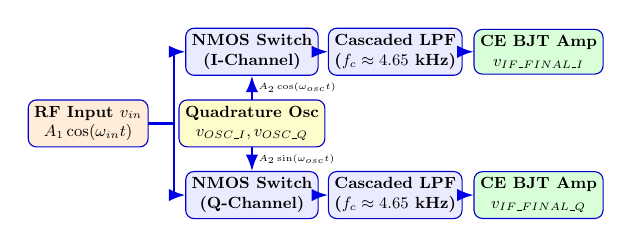
\begin{tikzpicture}[
      scale=0.65, every node/.style={transform shape},
      block/.style={draw=blue!80!black, rectangle, minimum height=0.8cm, minimum width=1.8cm, align=center, fill=blue!8, rounded corners=3pt, font=\small\bfseries},
      line/.style={draw=blue!90!black, -{Latex[scale=0.9]}, thick}
  ]
      % Left: RF Input
      \node [block, fill=orange!15] (rf) at (0, 0) {RF Input $v_{in}$\\$A_1\cos(\omega_{in}t)$};
      
      % Middle-Right: Mixers
      \node [block] (mixI) at (3.2, 1.4) {NMOS Switch\\(I-Channel)};
      \node [block] (mixQ) at (3.2, -1.4) {NMOS Switch\\(Q-Channel)};
      
      % Middle: Oscillator between paths
      \node [block, fill=yellow!20] (osc) at (3.2, 0) {Quadrature Osc\\$v_{OSC\_I}, v_{OSC\_Q}$};
      
      % Filters
      \node [block] (lpfI) at (6.0, 1.4) {Cascaded LPF\\($f_c \approx 4.65\text{ kHz}$)};
      \node [block] (lpfQ) at (6.0, -1.4) {Cascaded LPF\\($f_c \approx 4.65\text{ kHz}$)};
      
      % Amplifiers
      \node [block, fill=green!15] (ampI) at (8.8, 1.4) {CE BJT Amp\\$v_{IF\_FINAL\_I}$};
      \node [block, fill=green!15] (ampQ) at (8.8, -1.4) {CE BJT Amp\\$v_{IF\_FINAL\_Q}$};

      % Connections
      \path [line] (rf.east) -- ++(0.5,0) |- (mixI.west);
      \path [line] (rf.east) -- ++(0.5,0) |- (mixQ.west);
      
      \path [line] (osc.north) -- node[right, font=\tiny] {$A_2\cos(\omega_{osc}t)$} (mixI.south);
      \path [line] (osc.south) -- node[right, font=\tiny] {$A_2\sin(\omega_{osc}t)$} (mixQ.north);
      
      \path [line] (mixI) -- (lpfI);
      \path [line] (mixQ) -- (lpfQ);
      \path [line] (lpfI) -- (ampI);
      \path [line] (lpfQ) -- (ampQ);
  \end{tikzpicture}%
  }

  \vspace{0.05cm}
  \begin{block}{\small Quadrature Downconversion Mathematical Equations}
    \scriptsize
    \setlength{\abovedisplayskip}{2pt}
    \setlength{\belowdisplayskip}{2pt}
    \begin{align*}
      v_{IF_I} &= v_{in} \times v_{OSC\_I} = \frac{A_1 A_2}{2}\left[\cos((\omega_{in}-\omega_{osc})t) + \cos((\omega_{in}+\omega_{osc})t)\right] \\
               &\xrightarrow{\text{After LPF}} \mathbf{v_{IF\_FINAL\_I} = \frac{A_1 A_2}{2}\cos(\omega_{IF}t)} \\[0.05cm]
      v_{IF_Q} &= v_{in} \times v_{OSC\_Q} = \frac{A_1 A_2}{2}\left[\sin((\omega_{in}+\omega_{osc})t) - \sin((\omega_{in}-\omega_{osc})t)\right] \\
               &\xrightarrow{\text{After LPF}} \mathbf{v_{IF\_FINAL\_Q} = \frac{A_1 A_2}{2}\sin(\omega_{IF}t)}
    \end{align*}
  \end{block}
\end{frame}

\section{Quadrature Oscillator Design}

% Slide 6: Quadrature Oscillator Topology Selection
\begin{frame}{Quadrature Oscillator Topology Selection}
  \begin{columns}
    \begin{column}{0.56\textwidth}
      \small
      \textbf{3-Op-Amp Allpass Quadrature Topology:}
      \begin{itemize}
        \item Consists of two active \textbf{allpass filter stages} and one \textbf{inverting amplifier} with soft nonlinear feedback.
        \item \textbf{Why 3-Op-Amp Allpass over 2-Op-Amp Integrator?}
        \begin{itemize}
          \item \textit{Wide Bandwidth:} Allpass filters maintain unity gain ($G=1$) across high frequencies up to tens of MHz.
          \item \textit{Precise Quadrature:} Sampling between identical stages guarantees an exact $90^\circ$ phase shift.
          \item \textit{Amplitude Stability:} Uniform loop gain prevents envelope variation during frequency adjustments.
        \end{itemize}
      \end{itemize}
    \end{column}
    \begin{column}{0.44\textwidth}
      \centering
      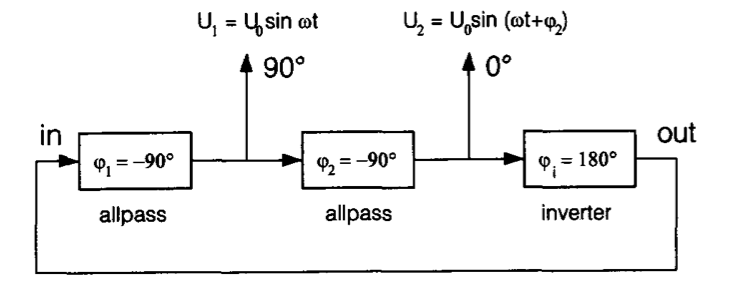
\includegraphics[width=0.85\linewidth]{../report/images/quad_topo.png} \\
      \vspace{0.02cm}
      \tiny Allpass Quadrature Oscillator Block Diagram.
    \end{column}
  \end{columns}
\end{frame}

% Slide 7: Oscillator Derivations & Calculations
\begin{frame}{Oscillator Derivations \& Component Calculations}
  \small
  \setlength{\abovedisplayskip}{2pt}
  \setlength{\belowdisplayskip}{2pt}
  \begin{itemize}
    \item \textbf{Allpass Phase Shift Transfer Function:}
    \begin{equation*}
      H(s) = \frac{sRC - 1}{sRC + 1} \implies \phi(f) = -2\arctan(2\pi f RC)
    \end{equation*}
    \item \textbf{Quadrature Oscillation Condition ($\phi = -90^\circ$ per stage):}
    \begin{equation*}
      2\pi f_{\text{osc}} RC = 1 \implies f_{\text{osc}} = \frac{1}{2\pi RC}
    \end{equation*}
    \item \textbf{Component Calculations for Target Frequencies ($C = 27\text{ pF}$):}
    \begin{itemize}
      \item For $f_{\text{osc}} = 150\text{ kHz}$: $R = \frac{1}{2\pi (150\text{ k})(27\text{ p})} \approx \mathbf{39.3\text{ k}\Omega}$
      \item For $f_{\text{osc}} = 200\text{ kHz}$: $R = \frac{1}{2\pi (200\text{ k})(27\text{ p})} \approx \mathbf{29.5\text{ k}\Omega}$
    \end{itemize}
    \item \textbf{Supply Voltages ($V_{DD}, V_{SS}$):} $\pm 15\text{ V}$ supplies provide wide linear operating range for standard UA741 op-amps to yield the requested $1\text{ V}_{\text{pp}}$ ($500\text{ mV}_{\text{peak}}$) swing.
  \end{itemize}
\end{frame}

% Slide 8: Diode Feedback & Asymmetry Justification
\begin{frame}{Diode Feedback \& Asymmetry Justification}
  \begin{columns}
    \begin{column}{0.5\textwidth}
      \begin{block}{Nonlinear Diode Network}
        \begin{itemize}
          \item Diodes (D1, D3) and resistors (R9, R10) in inverter (op3) feedback path.
          \item \textbf{Startup:} Initial gain $> 1$ ($R_4/R_3 > 1$) ensures rapid startup from noise.
          \item \textbf{Soft Clamping:} At $1\text{ V}_{\text{pp}}$, diodes conduct, reducing effective gain to lock $A\beta = 1$.
        \end{itemize}
      \end{block}
    \end{column}
    \begin{column}{0.5\textwidth}
      \begin{block}{Justification of Asymmetric Tuning}
        \begin{itemize}
          \item Symmetric SPICE values led to waveform distortion in physical breadboard realization.
          \item UA741 high-frequency internal poles introduce parasitic phase lag at $>150\text{ kHz}$.
          \item Asymmetric tuning ($R_8 = 432\,\Omega, R_5 = 15.2\text{ k}\Omega$) compensates for parasitics and stage loading.
        \end{itemize}
      \end{block}
    \end{column}
  \end{columns}
\end{frame}

% Slide 9: LTSpice Simulation of Quadrature Oscillator
\begin{frame}{LTSpice Simulation -- Schematic \& Transient Waveforms}
  \begin{columns}
    \begin{column}{0.5\textwidth}
      \centering
      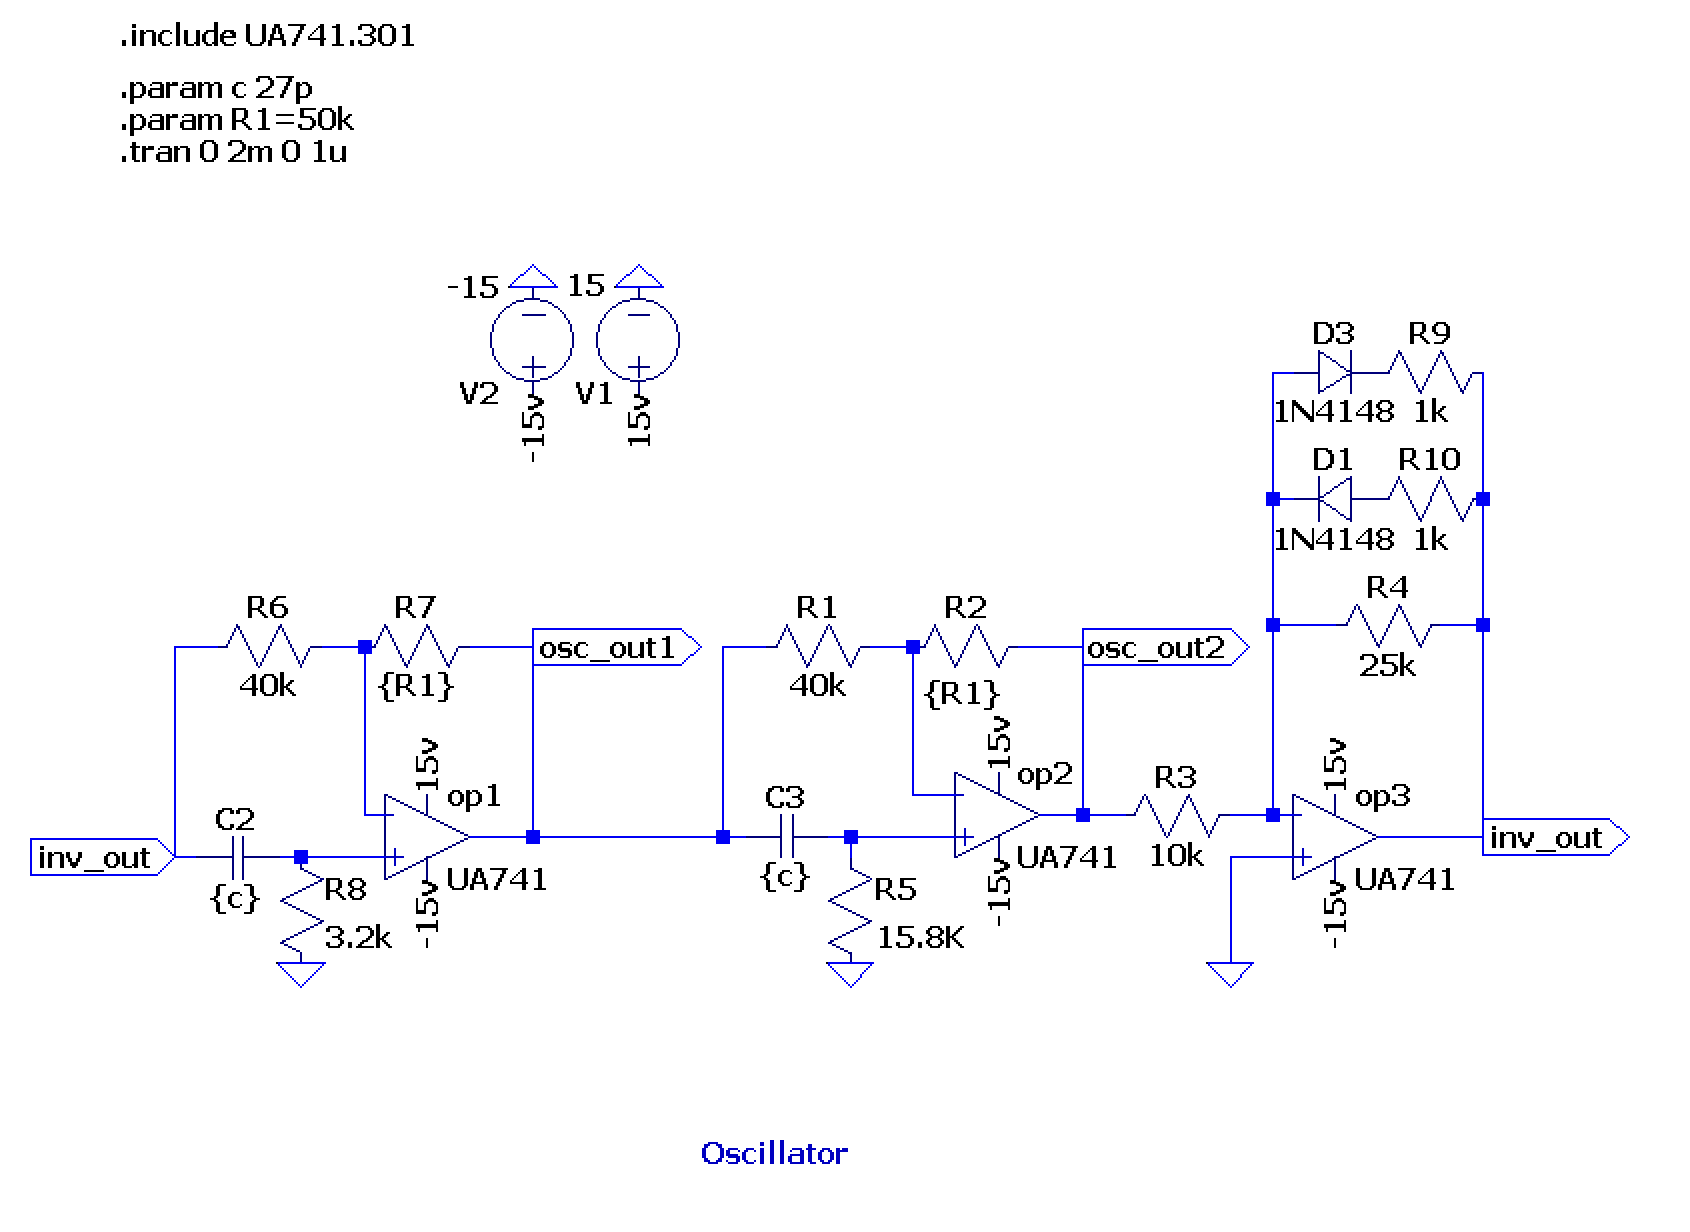
\includegraphics[width=\linewidth]{../report/images/osc_ltspice.png}
      \vspace{0.1cm}
      \tiny (a) Complete UA741 Quadrature Oscillator Schematic.
    \end{column}
    \begin{column}{0.5\textwidth}
      \centering
      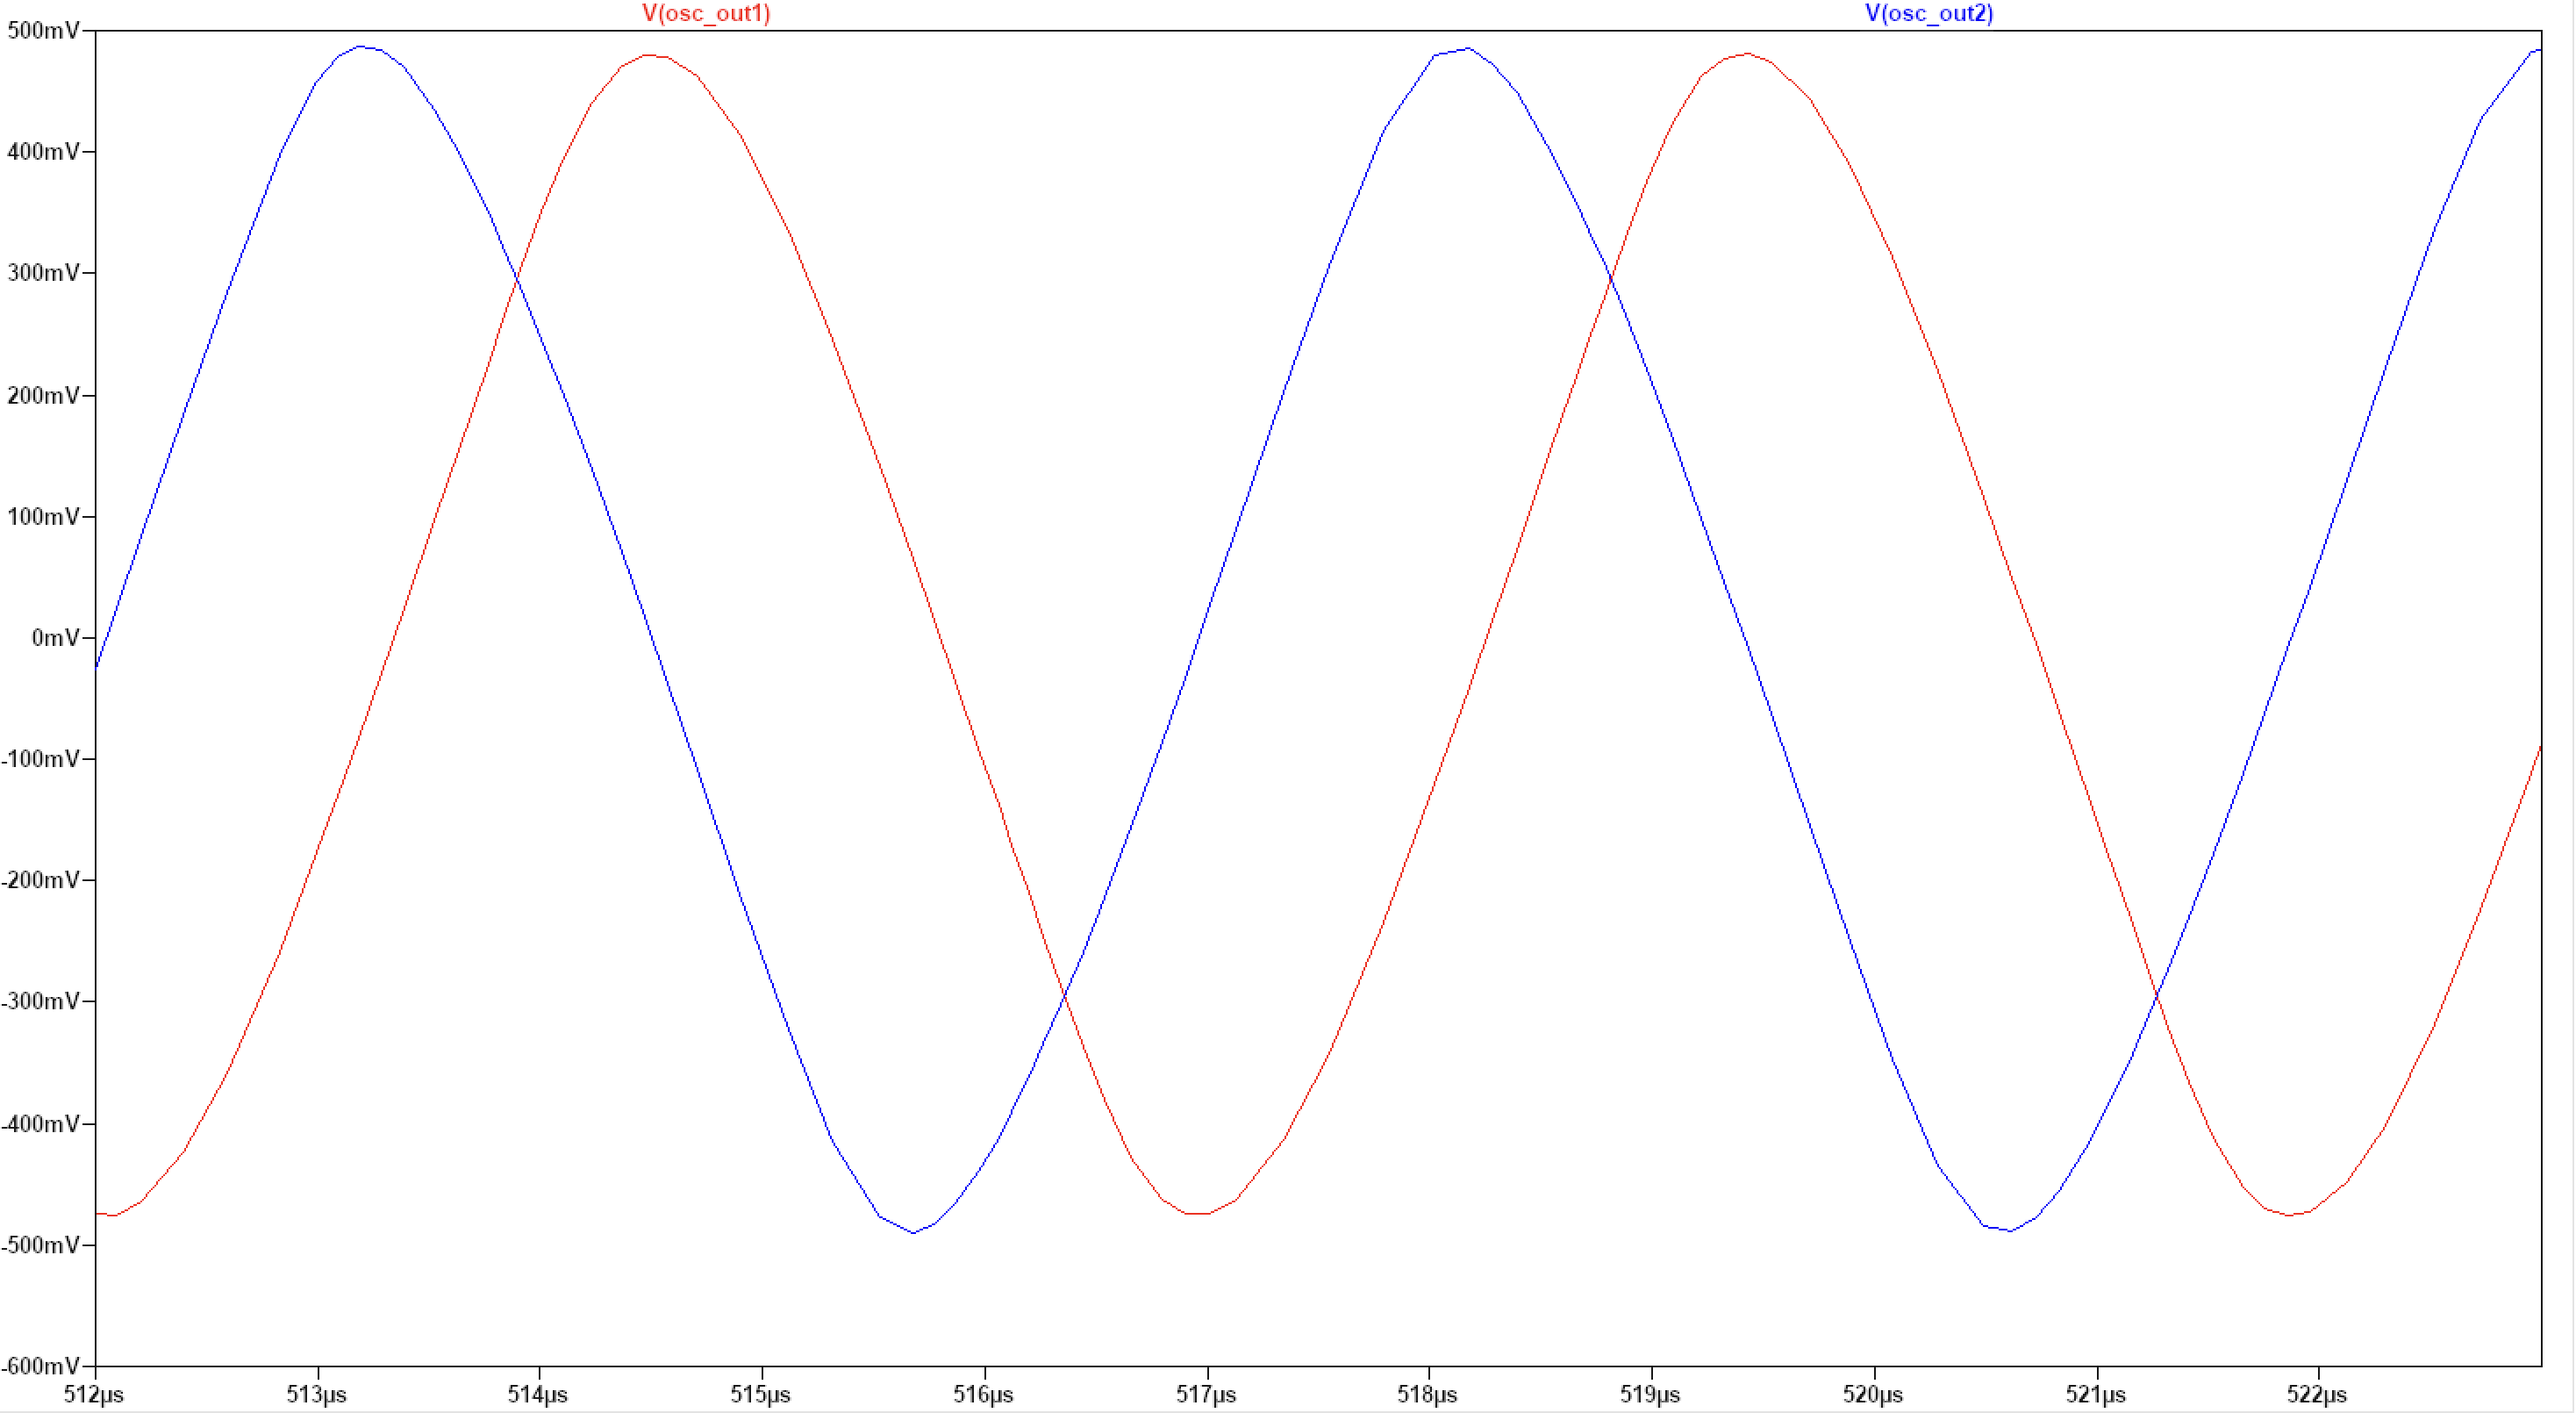
\includegraphics[width=\linewidth]{../report/images/osc-outputs1.png}
      \vspace{0.1cm}
      \tiny (b) Transient Simulation: Period $T=5.424\,\mu\text{s}$, phase shift $= -268.49^\circ$ ($+91.51^\circ$).
    \end{column}
  \end{columns}
  \vspace{0.2cm}
  \scriptsize
  \textbf{Verification:} Output swing stabilizes precisely at $1\text{ V}_{\text{pp}}$ ($500\text{ mV}_{\text{peak}}$) with clean $90^\circ$ phase shift.
\end{frame}

% Slide 10: Phase Shift & Spectral Purity Analysis
\begin{frame}{Phase Measurement \& FFT Spectral Analysis}
  \begin{columns}
    \begin{column}{0.5\textwidth}
      \centering
      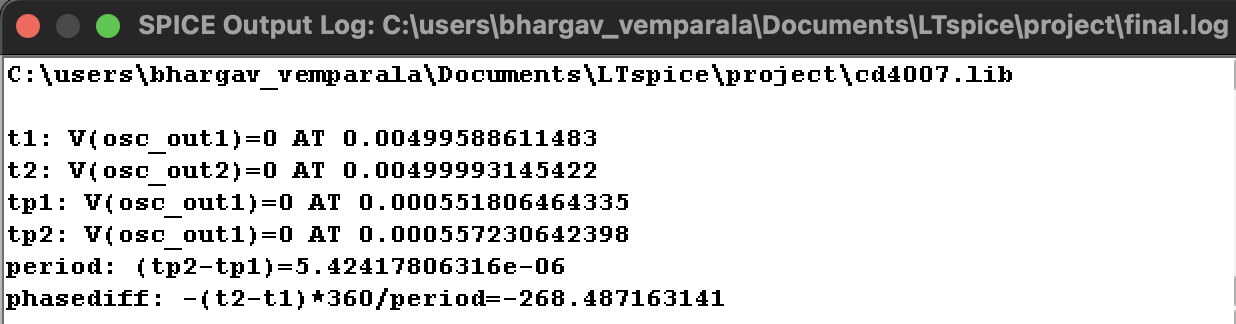
\includegraphics[width=0.88\linewidth]{../report/images/osc-phase-calc.png}
      \vspace{0.1cm}
      \tiny SPICE Error Log phase calculation verifying $91.51^\circ$ phase shift between I and Q.
    \end{column}
    \begin{column}{0.5\textwidth}
      \centering
      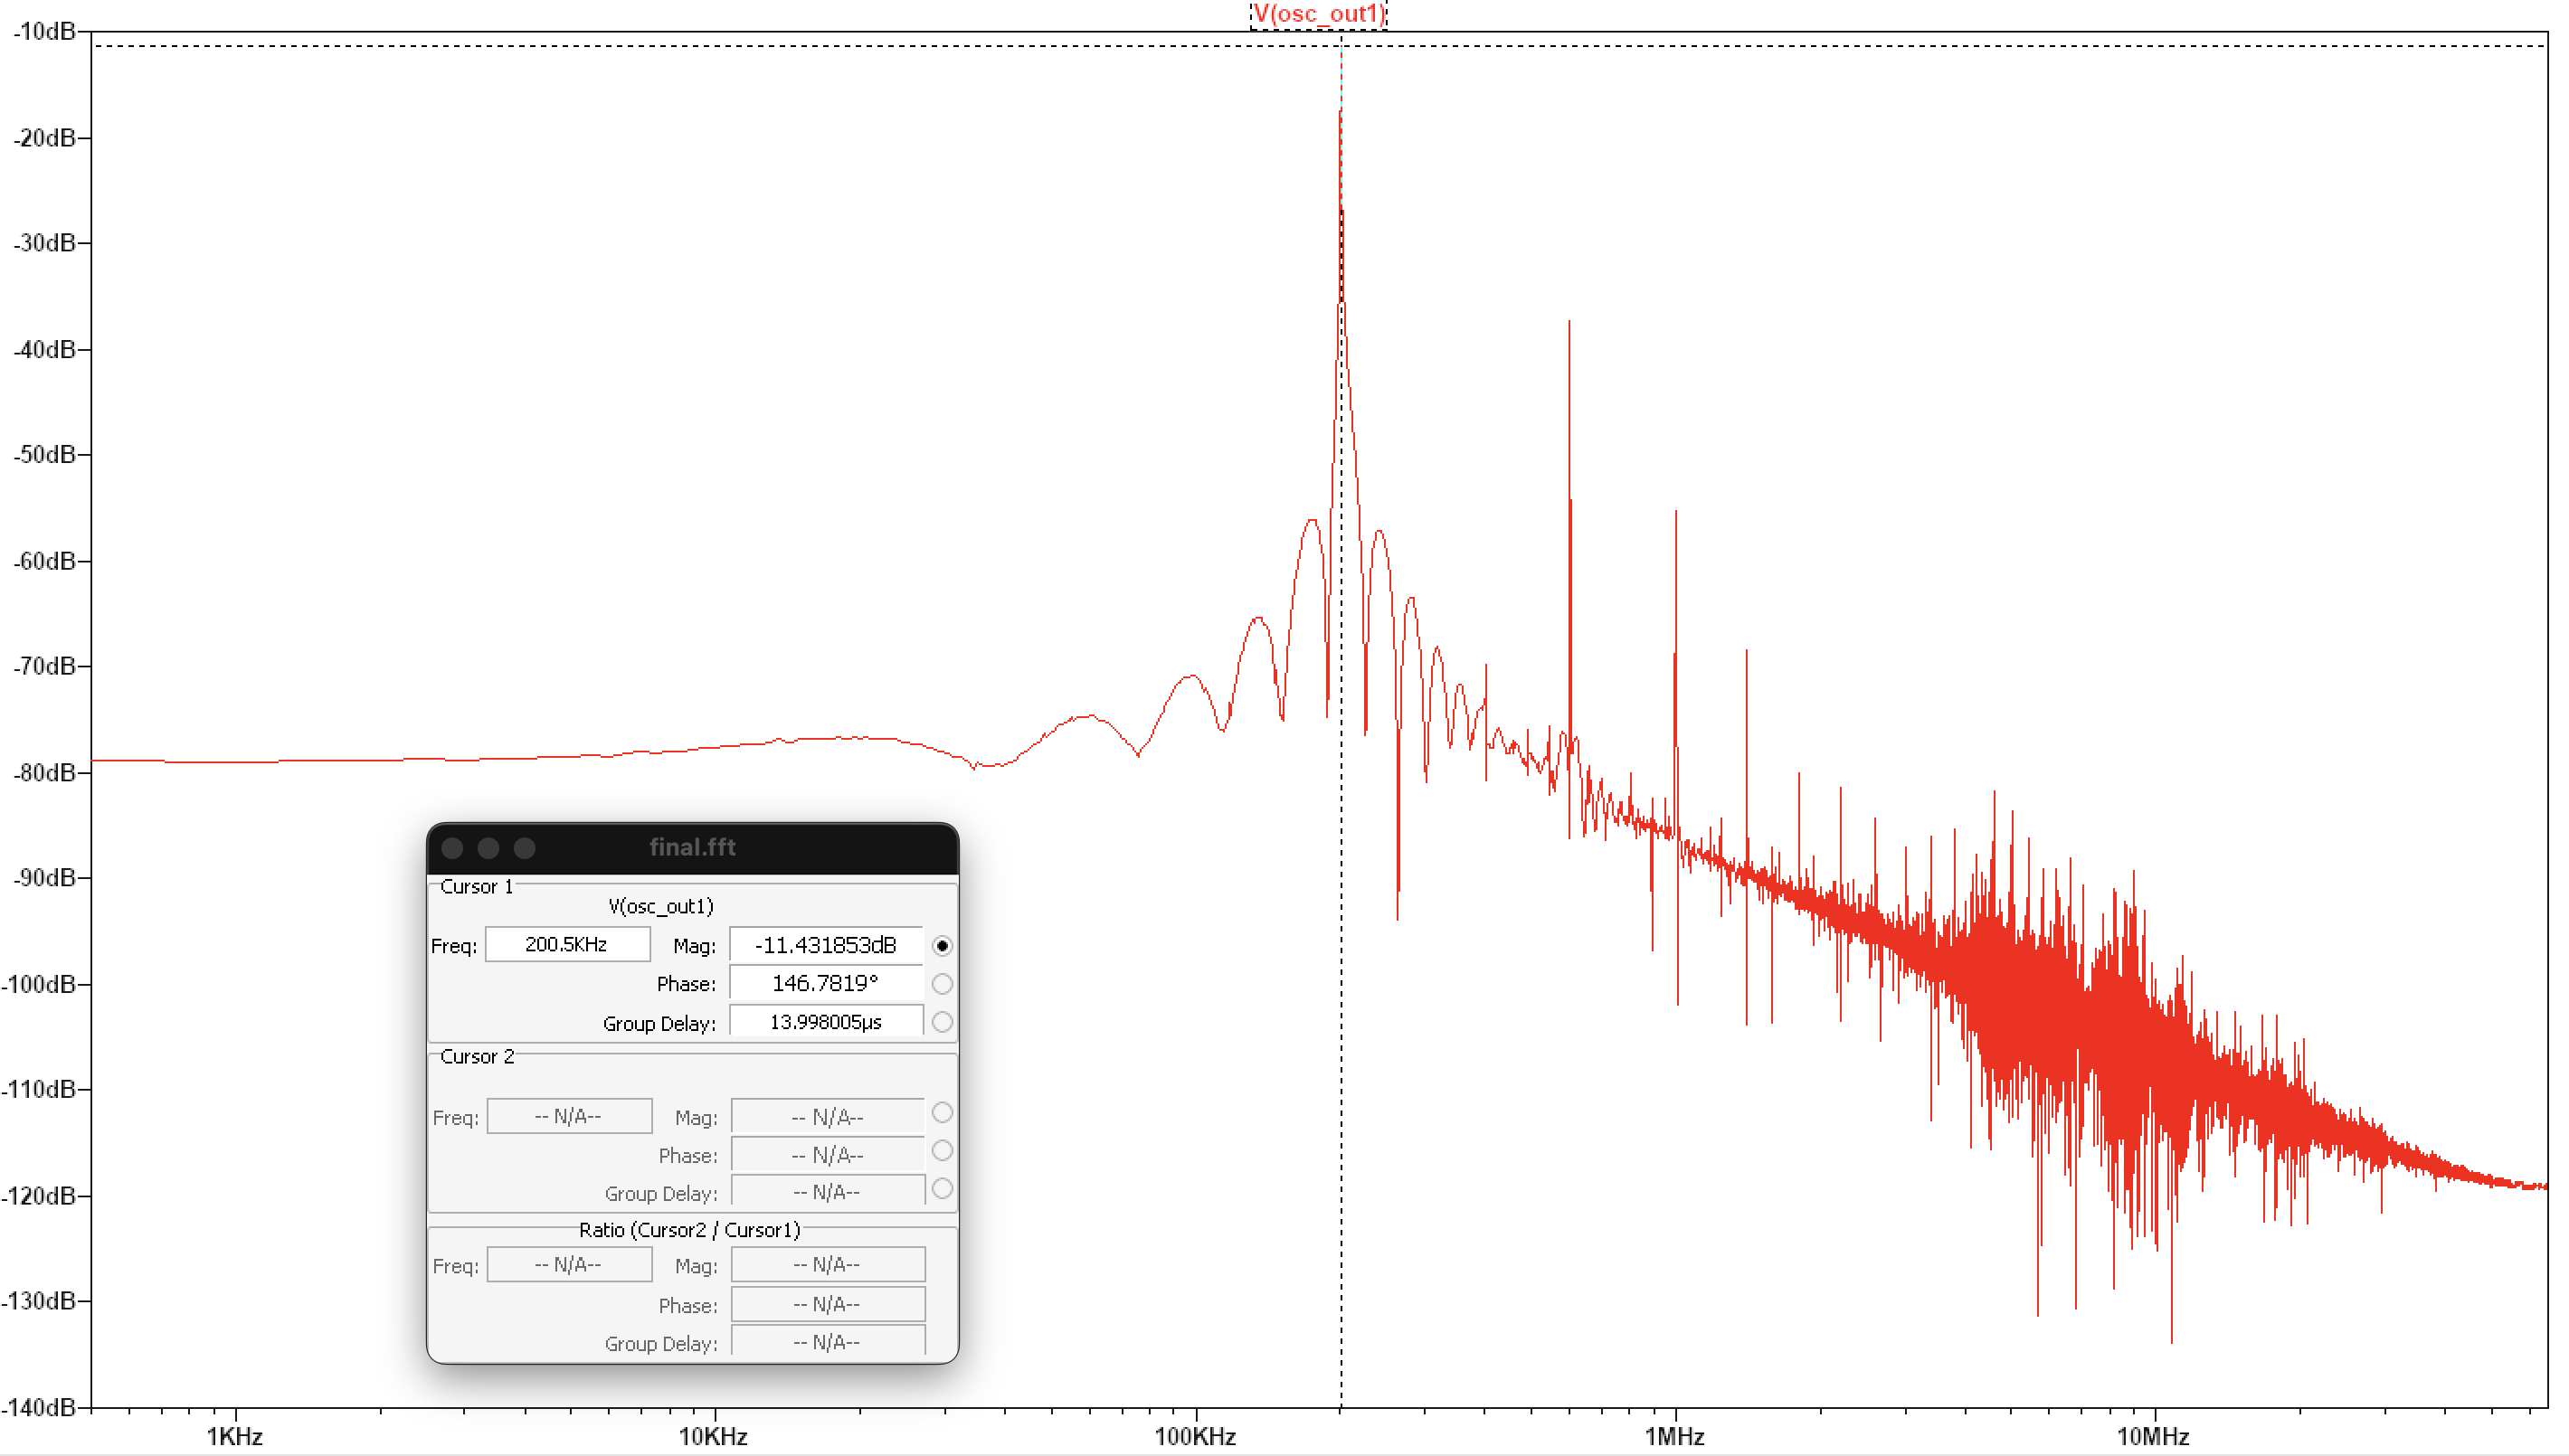
\includegraphics[width=\linewidth]{../report/images/osc-fft.png}
      \vspace{0.1cm}
      \tiny FFT Spectrum of $v_{OSC\_I}$: Strong peak at $200.5\text{ kHz}$, magnitude $-11.43\text{ dB}$, phase $146.78^\circ$.
    \end{column}
  \end{columns}
\end{frame}

% Slide 11: Lab Realization & Resistor Comparison
\begin{frame}{Hardware Realization (741 ICs) \& Parameter Tweaks}
  \begin{columns}
    \begin{column}{0.48\textwidth}
      \centering
      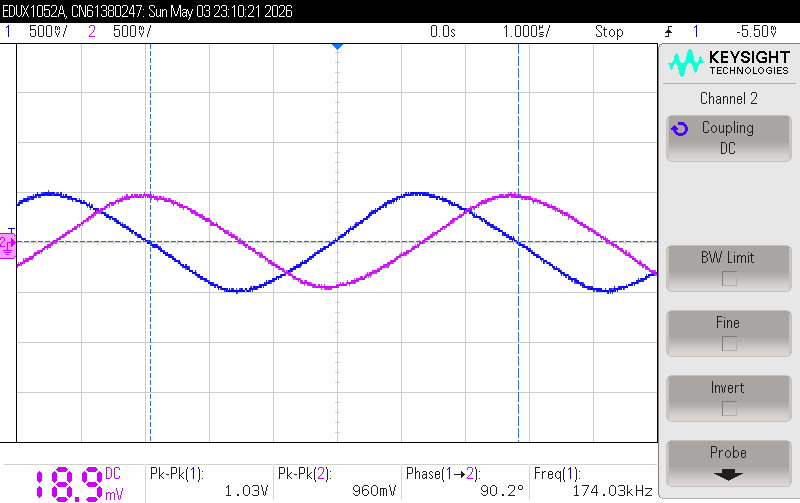
\includegraphics[width=\linewidth]{../report/images/oscillator-output-sin-cos.png}
      \vspace{0.1cm}
      \tiny DSO Measurement: Realized $v_{OSC\_I}$ \& $v_{OSC\_Q}$ waveforms.
    \end{column}
    \begin{column}{0.52\textwidth}
      \begin{table}
        \centering\tiny
        \caption{Resistor Comparison: SPICE vs. Lab Potentiometer Method}
        \resizebox{\linewidth}{!}{%
        \begin{tabular}{lcc}
          \toprule
          \textbf{Component} & \textbf{SPICE Value ($\Omega$)} & \textbf{Real Life Value ($\Omega$)} \\
          \midrule
          $R_1 / R_7$ & $40\text{ k} / 50\text{ k}$ & $50\text{ k} / 47\text{ k}$ \\
          $R_2 / R_6$ & $50\text{ k} / 40\text{ k}$ & $47\text{ k} / 39.2\text{ k}$ \\
          $R_3 / R_4$ & $10\text{ k} / 25\text{ k}$ & $10\text{ k} / 17.6\text{ k}$ \\
          $R_5 / R_8$ & $15.8\text{ k} / 3.2\text{ k}$ & $15.2\text{ k} / 432$ \\
          $R_9 / R_{10}$ & $1\text{ k} / 1\text{ k}$ & $2.2\text{ k} / 2.2\text{ k}$ \\
          \bottomrule
        \end{tabular}%
        }
      \end{table}
      \centering
      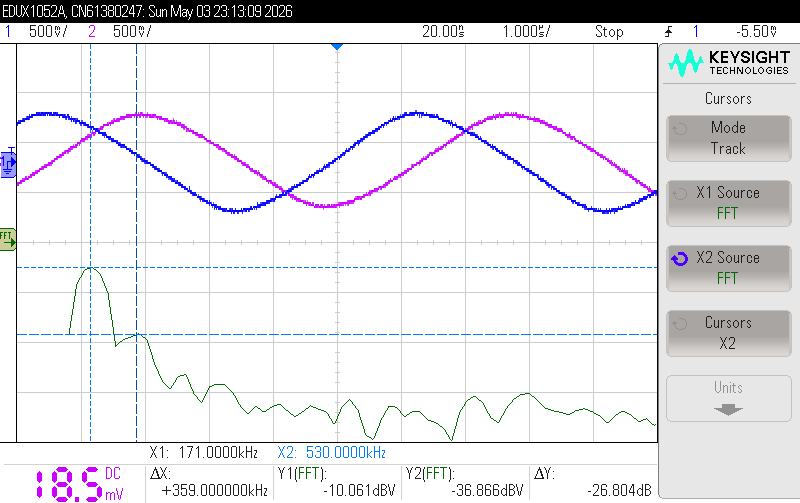
\includegraphics[width=0.7\linewidth]{../report/images/oscillator-ouput-sin-cos-fft.png}
      \vspace{0.05cm}
      \tiny DSO FFT confirming hardware spectral purity.
    \end{column}
  \end{columns}
\end{frame}

\section{Active NMOS Switch Mixer Design}

% Slide 12: Active NMOS Switch Topology & MOSFET Sizing
\begin{frame}{Switch (Mixer) Topology \& MOSFET Optimization}
  \begin{itemize}
    \item \textbf{Active NMOS Switch Topology:} Passive NMOS switch operating in deep triode region.
    \begin{itemize}
      \item RF Input ($v_{in} = 100\text{ mV}$) connected to Drain; LO ($v_{OSC}$) AC-coupled to Gate.
      \item Intermediate Frequency output ($v_{IF}$) taken at Drain across $R_L = 1\text{ k}\Omega$.
    \end{itemize}
    \item \textbf{MOSFET Parameter Optimization ($180\text{ nm}$ CMOS Node):}
    \begin{itemize}
      \item Channel Length: $L = 0.18\,\mu\text{m}$ (minimum feature size).
      \item Width $W = 20\,\mu\text{m}$ for target $R_{\text{on}} \approx 50\,\Omega$ ($V_{\text{GS}} - V_{\text{th}} = 0.6\text{ V}$):
      \begin{align*}
        \frac{W}{L} &= \frac{1}{R_{\text{on}}\cdot \mu_n C_{\text{ox}}(V_{\text{GS}}-V_{\text{th}})} = \frac{1}{50 \cdot 300\,\mu \cdot 0.6} \approx 111.1 \\
        &\implies W = 111.1 \times 0.18\,\mu\text{m} \approx \mathbf{20\,\mu\text{m}}
      \end{align*}
    \end{itemize}
    \item \textbf{LTspice Geometric Parasitics ($Y = 0.18\,\mu\text{m}$):}
    \begin{itemize}
      \item Source/Drain Area: $A_S = A_D = W \times Y = 3.6\text{ p}$ (\texttt{3.6p})
      \item Source/Drain Perimeter: $P_S = P_D = W + 2Y = 20.36\,\mu\text{m}$ (\texttt{20.36u})
    \end{itemize}
  \end{itemize}
\end{frame}

% Slide 13: Mixer LTSpice Schematic & Component Rationale
\begin{frame}{Mixer LTSpice Schematic \& Component Values}
  \begin{columns}
    \begin{column}{0.48\textwidth}
      \centering
      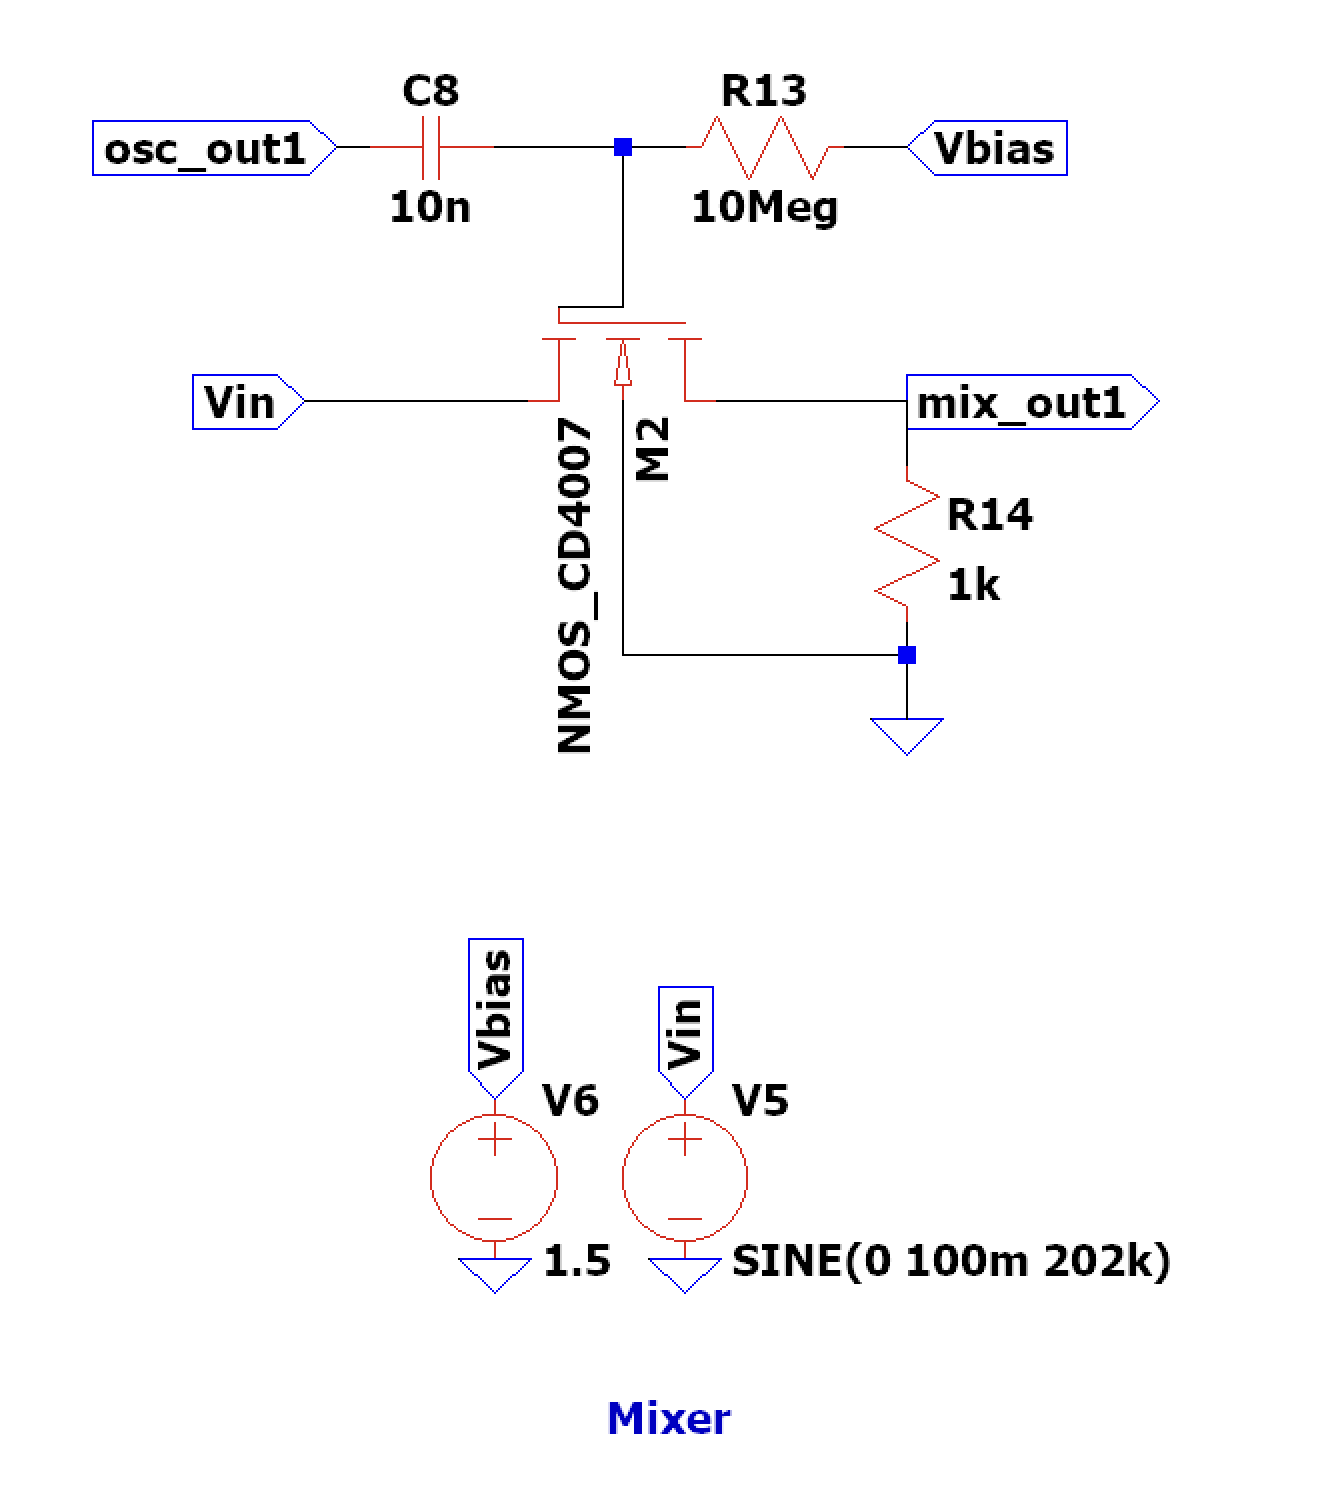
\includegraphics[width=\linewidth]{../report/images/Mixer_circ.png}
      \vspace{0.1cm}
      \tiny LTSpice NMOS Switch Mixer Schematic.
    \end{column}
    \begin{column}{0.52\textwidth}
      \begin{table}
        \centering\tiny
        \caption{Mixer Component Summary}
        \resizebox{\linewidth}{!}{%
        \begin{tabular}{lcp{3.2cm}}
          \toprule
          \textbf{Component} & \textbf{Value} & \textbf{Rationale} \\
          \midrule
          $M_1$ & NMOS ($20\text{u}/0.18\text{u}$) & Core switching element. \\
          $R_{\text{BIAS}}$ & $10\text{ M}\Omega$ & Prevents AC loading on LO gate node. \\
          $C_C$ & $10\text{ nF}$ & AC couples LO signal; blocks DC. \\
          $R_L$ & $1\text{ k}\Omega$ & Standard load for gain/bandwidth balance. \\
          $V_{\text{BIAS}}$ & $0.6\text{ V} - 0.8\text{ V}$ & Sets gate near $V_{\text{th}}$ for sharp switching. \\
          \bottomrule
        \end{tabular}%
        }
      \end{table}
    \end{column}
  \end{columns}
\end{frame}

% Slide 14: Mixer Mathematical Derivation & Frequency Conversion
\begin{frame}{Mixer Mathematical Derivations \& Downconversion}
  \begin{itemize}
    \item \textbf{Square-Wave Switching Expansion:}
    \begin{equation*}
      s(t) = \frac{1}{2} + \frac{2}{\pi}\sum_{n=1,3,5\dots}^{\infty}\frac{\sin(n\omega_{\text{osc}}t)}{n}
    \end{equation*}
    \item \textbf{Product-to-Sum Multiplication:}
    \begin{align*}
      v_{out}(t) &\approx A_{in}\cos(\omega_{in}t) \cdot \frac{2}{\pi}\sin(\omega_{\text{osc}}t) \\
                 &= \frac{A_{in}}{\pi}\left[\sin((\omega_{\text{osc}} - \omega_{in})t) + \sin((\omega_{\text{osc}} + \omega_{in})t)\right]
    \end{align*}
    \item \textbf{Extracted Frequencies ($f_{\text{osc}} = 170\text{ kHz}, f_{\text{in}} = 165\text{ kHz}$):}
    \begin{itemize}
      \item \textbf{Downconverted IF Component:} $f_{\text{IF}} = |f_{\text{osc}} - f_{\text{in}}| = |170\text{ k} - 165\text{ k}| = 5\text{ kHz}$
      \item \textbf{Sum Component (Filtered by LPF):} $f_{\text{sum}} = 170\text{ k} + 165\text{ k} = 335\text{ kHz}$
    \end{itemize}
  \end{itemize}
\end{frame}

% Slide 15: Mixer Frequency Sweep Analysis (165 kHz - 169 kHz)
\begin{frame}{Frequency Sweep Analysis ($f_{\text{IN}} < f_{\text{OSC}}$: 165--169 kHz)}
  \begin{columns}
    \begin{column}{0.33\textwidth}
      \centering
      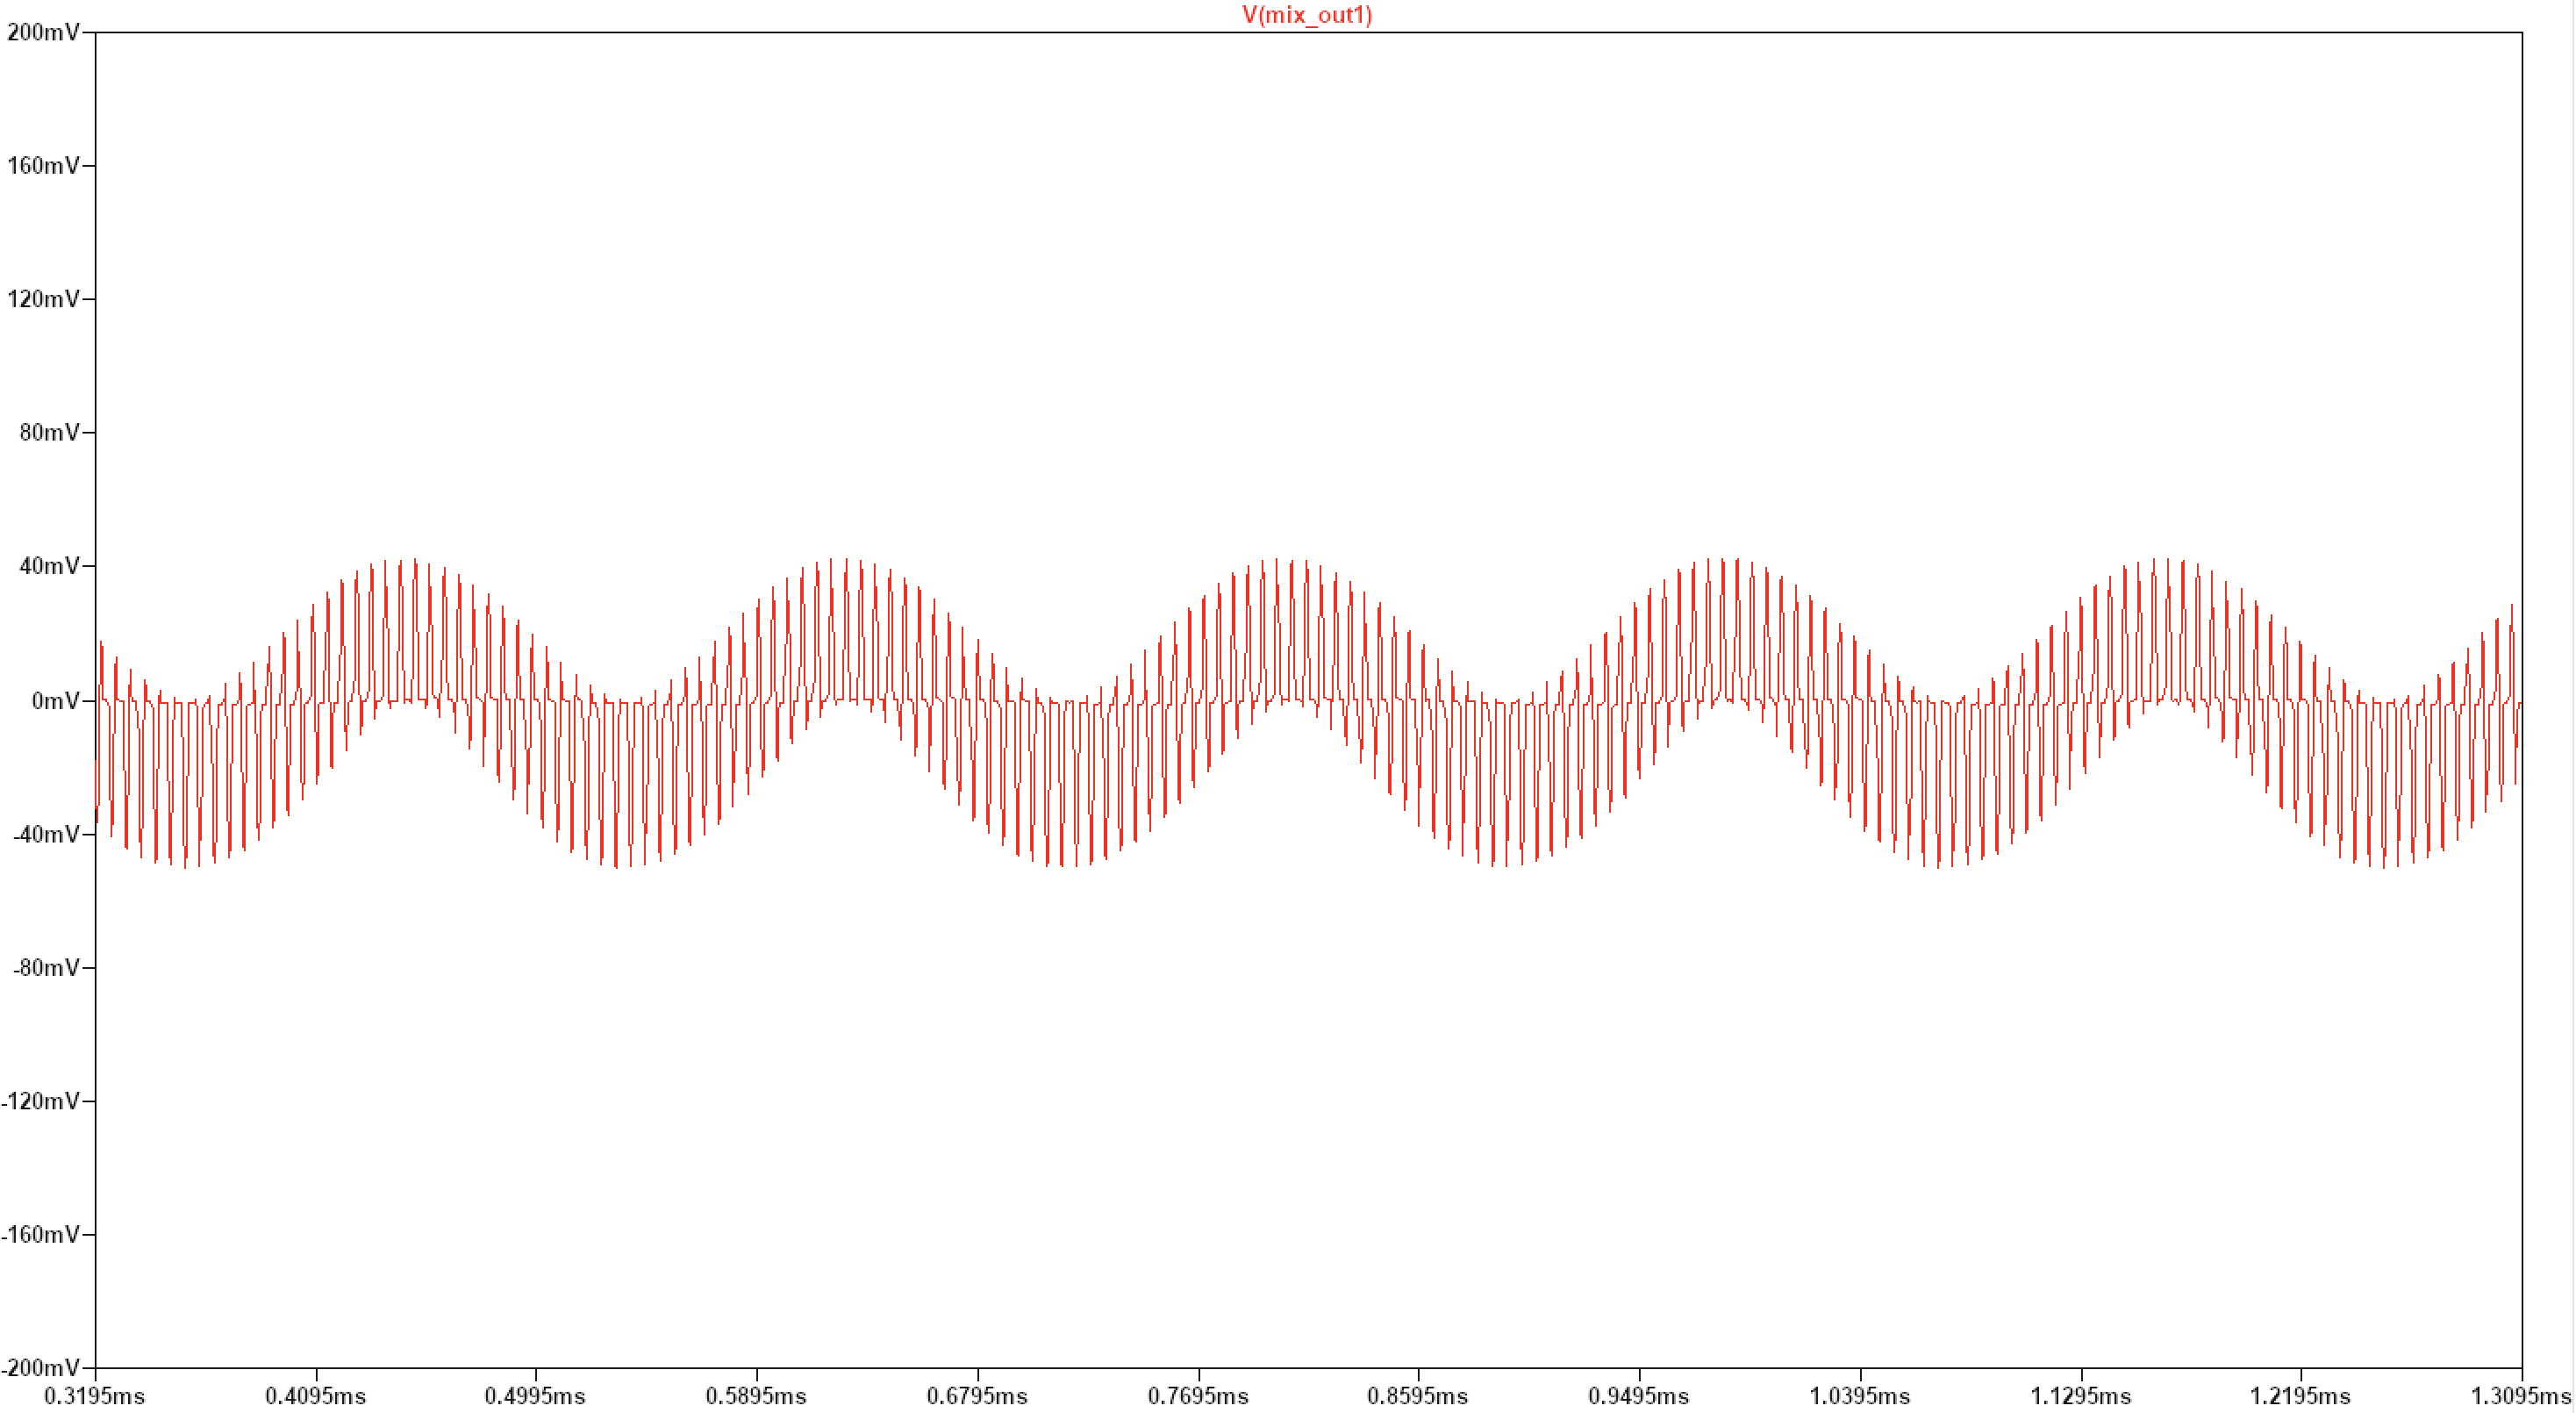
\includegraphics[width=\linewidth]{../report/images/165k-t.png} \\
      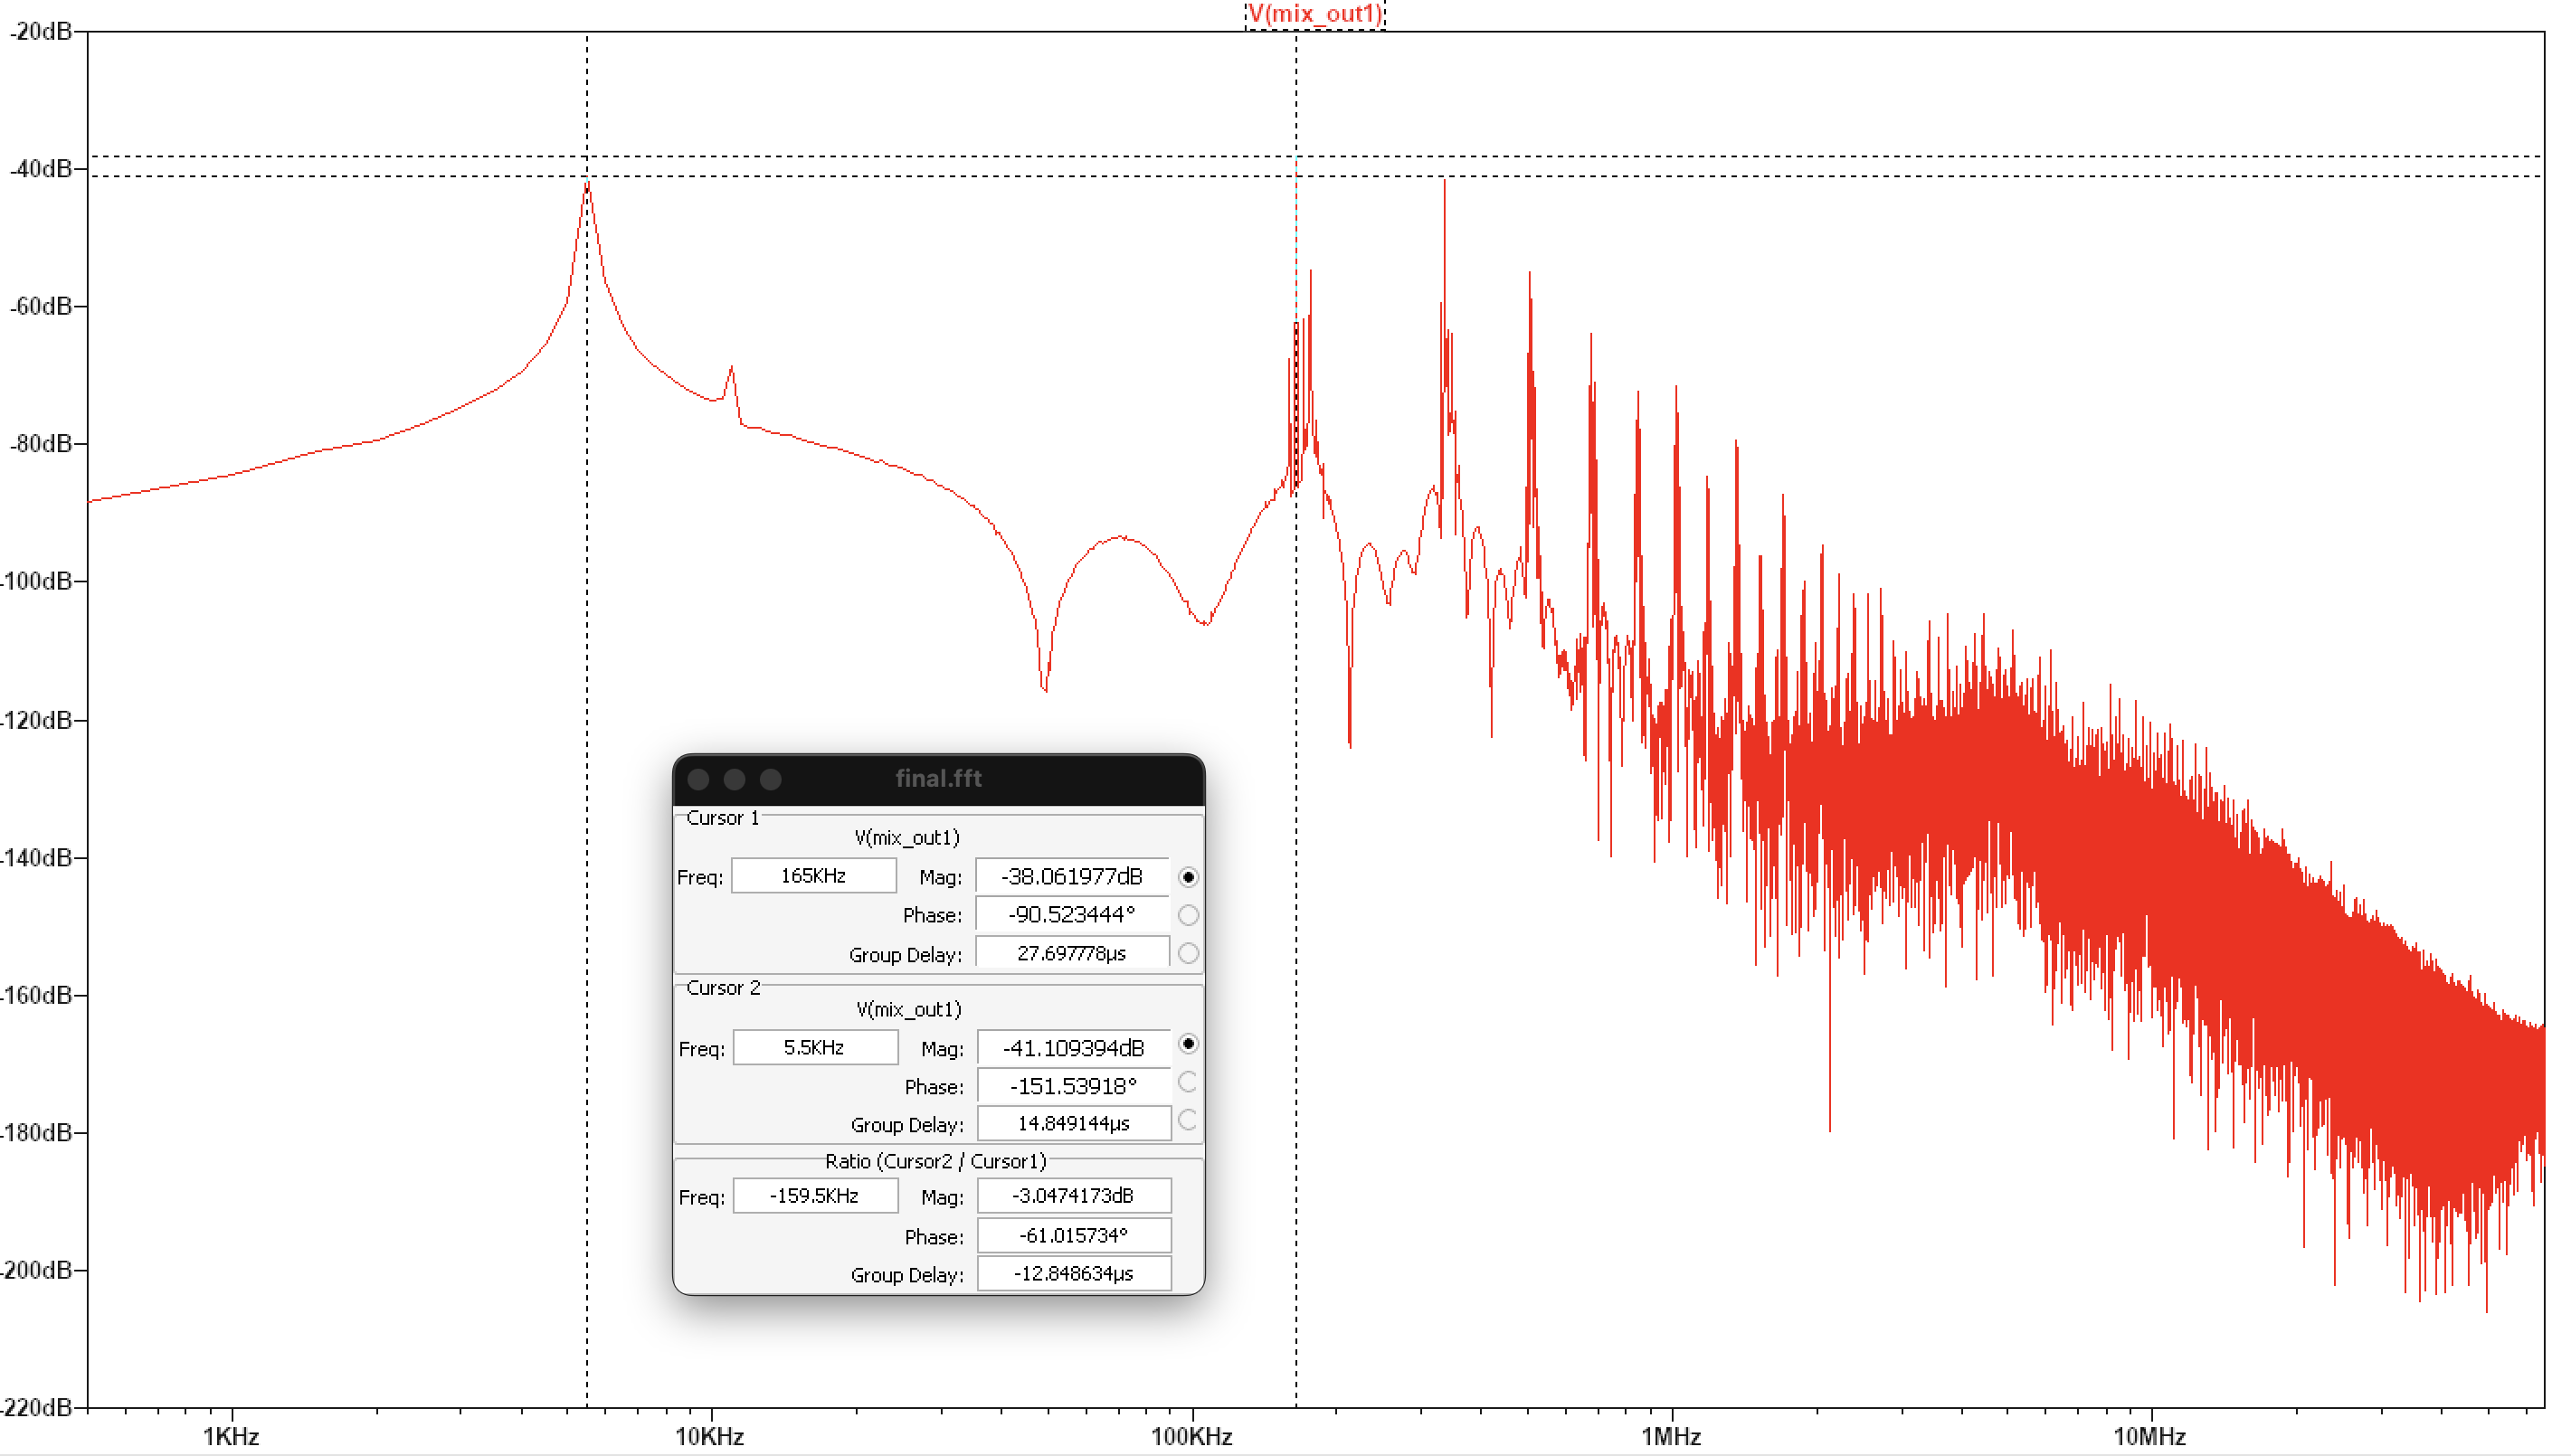
\includegraphics[width=\linewidth]{../report/images/165k-fft.png}
      \vspace{0.05cm}
      \tiny \textbf{$165\text{ kHz}$ Input:} $f_{\text{IF}} = 5\text{ kHz}$
    \end{column}
    \begin{column}{0.33\textwidth}
      \centering
      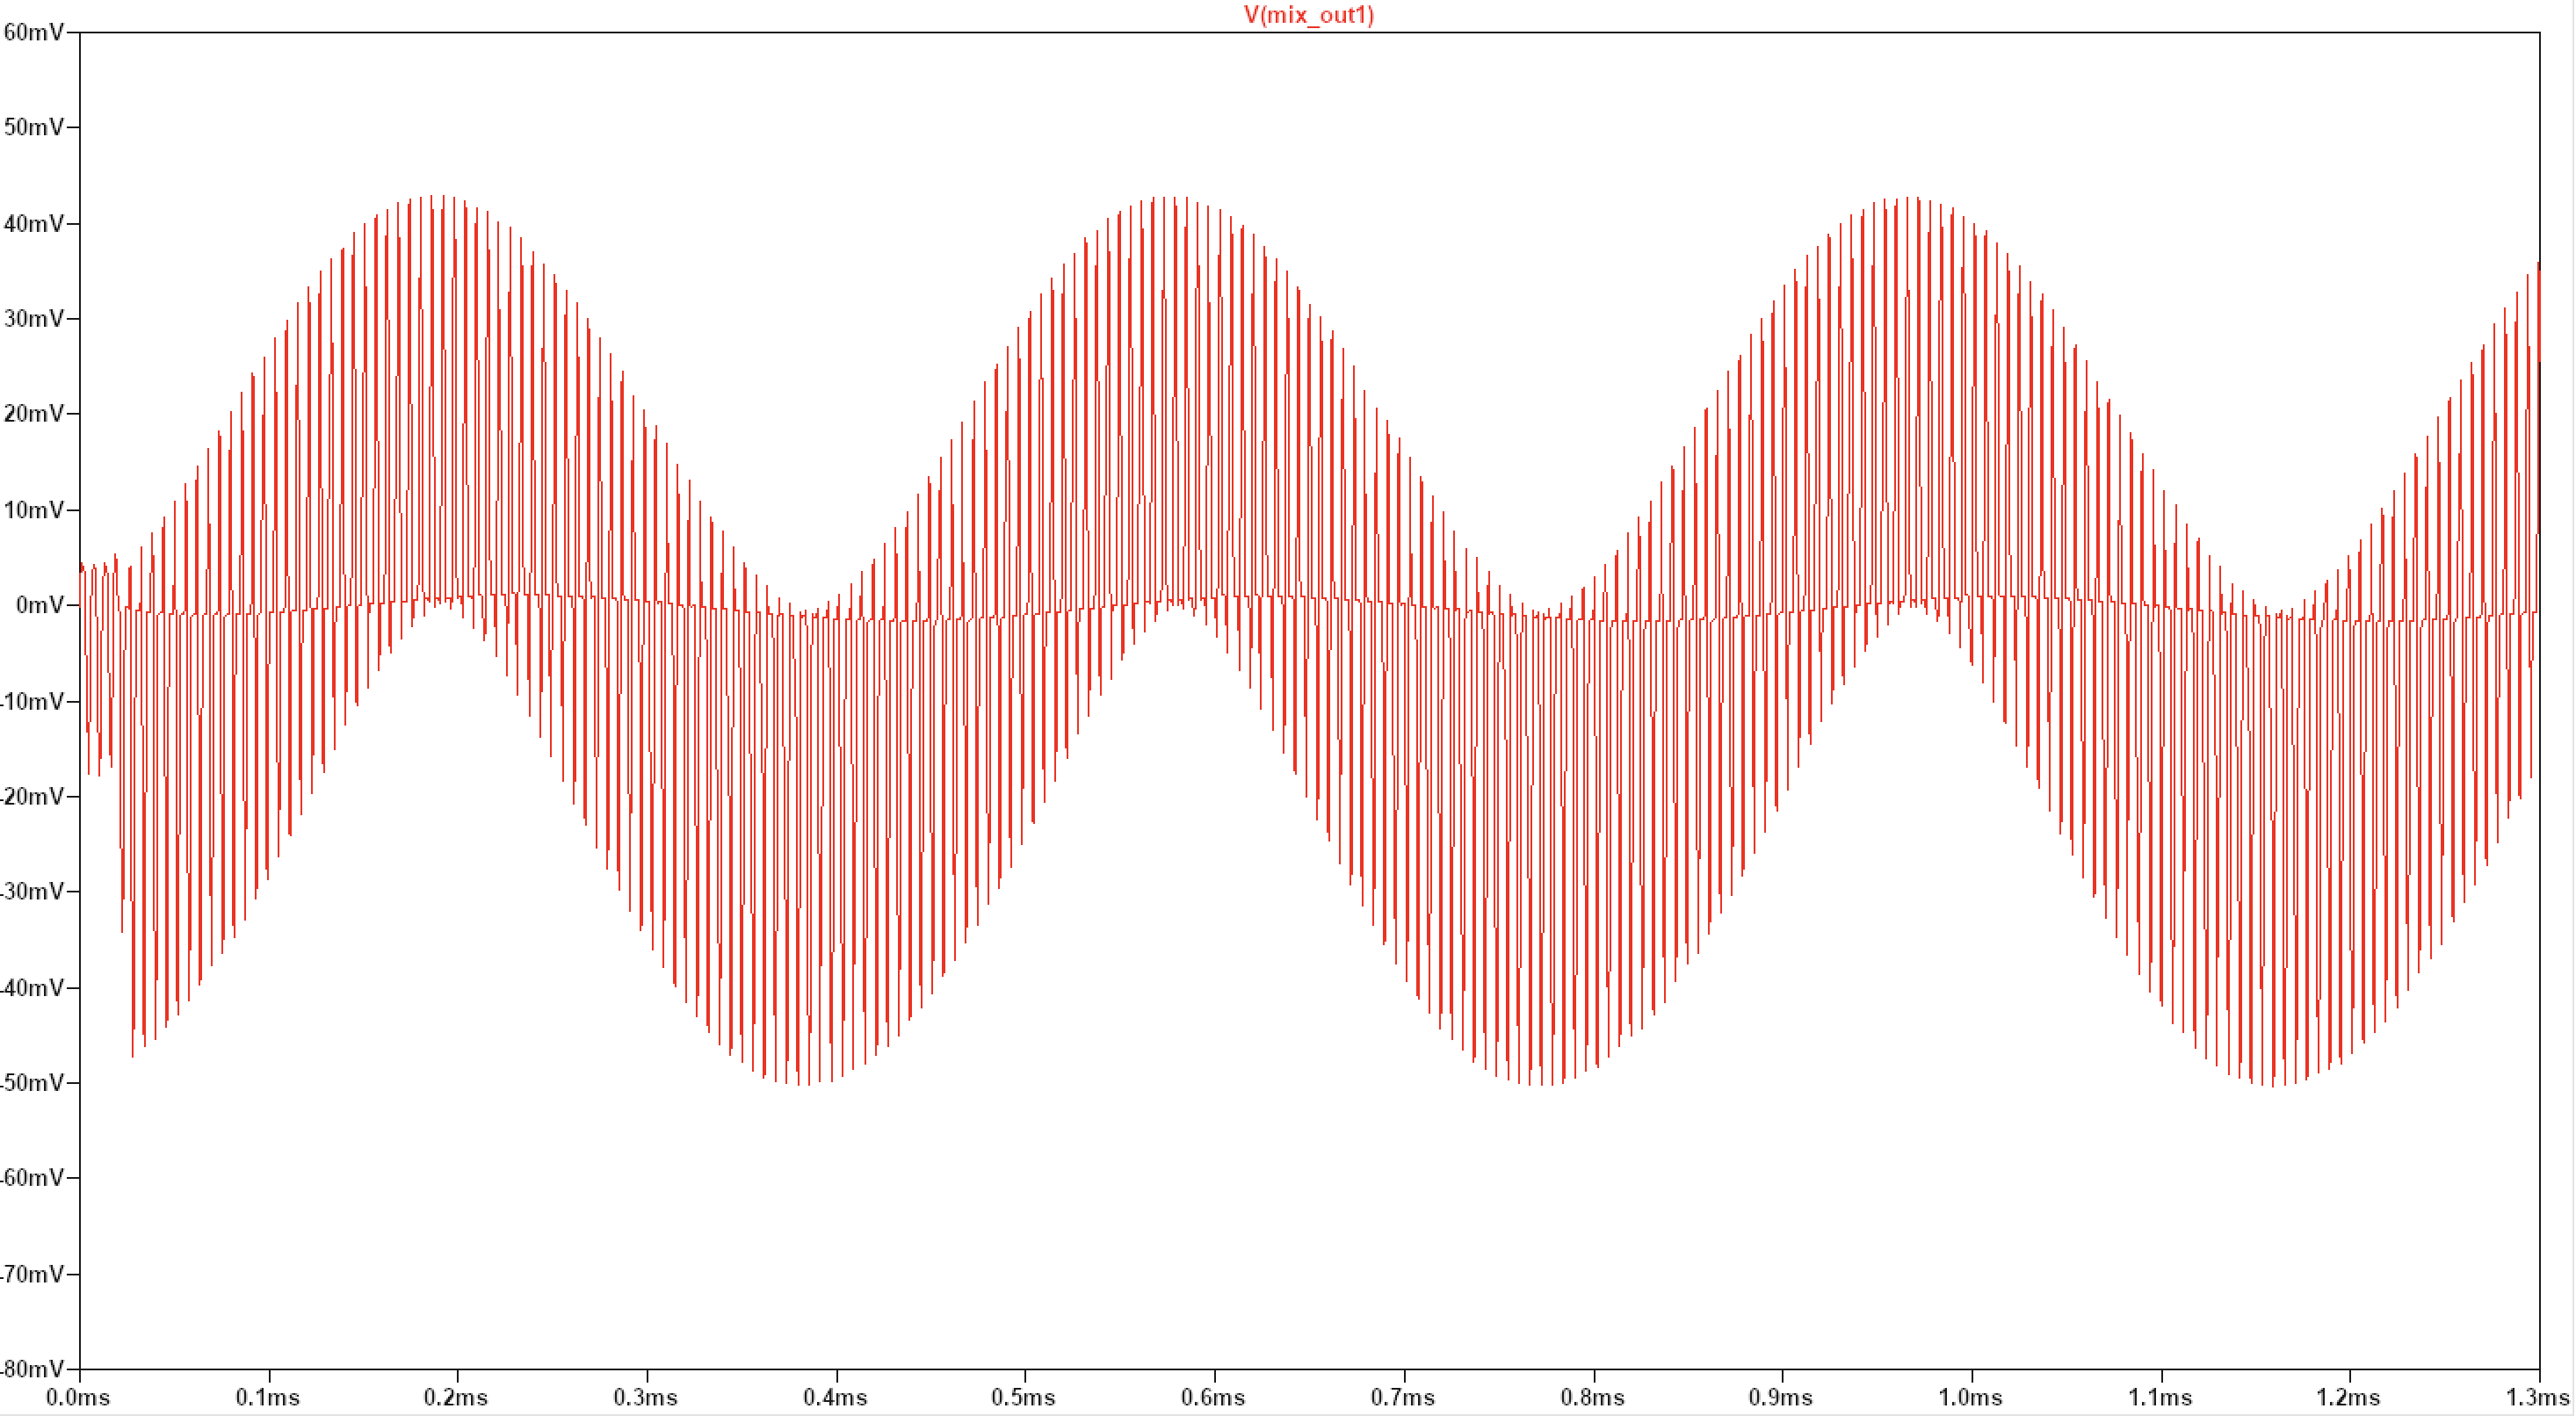
\includegraphics[width=\linewidth]{../report/images/168k-t.png} \\
      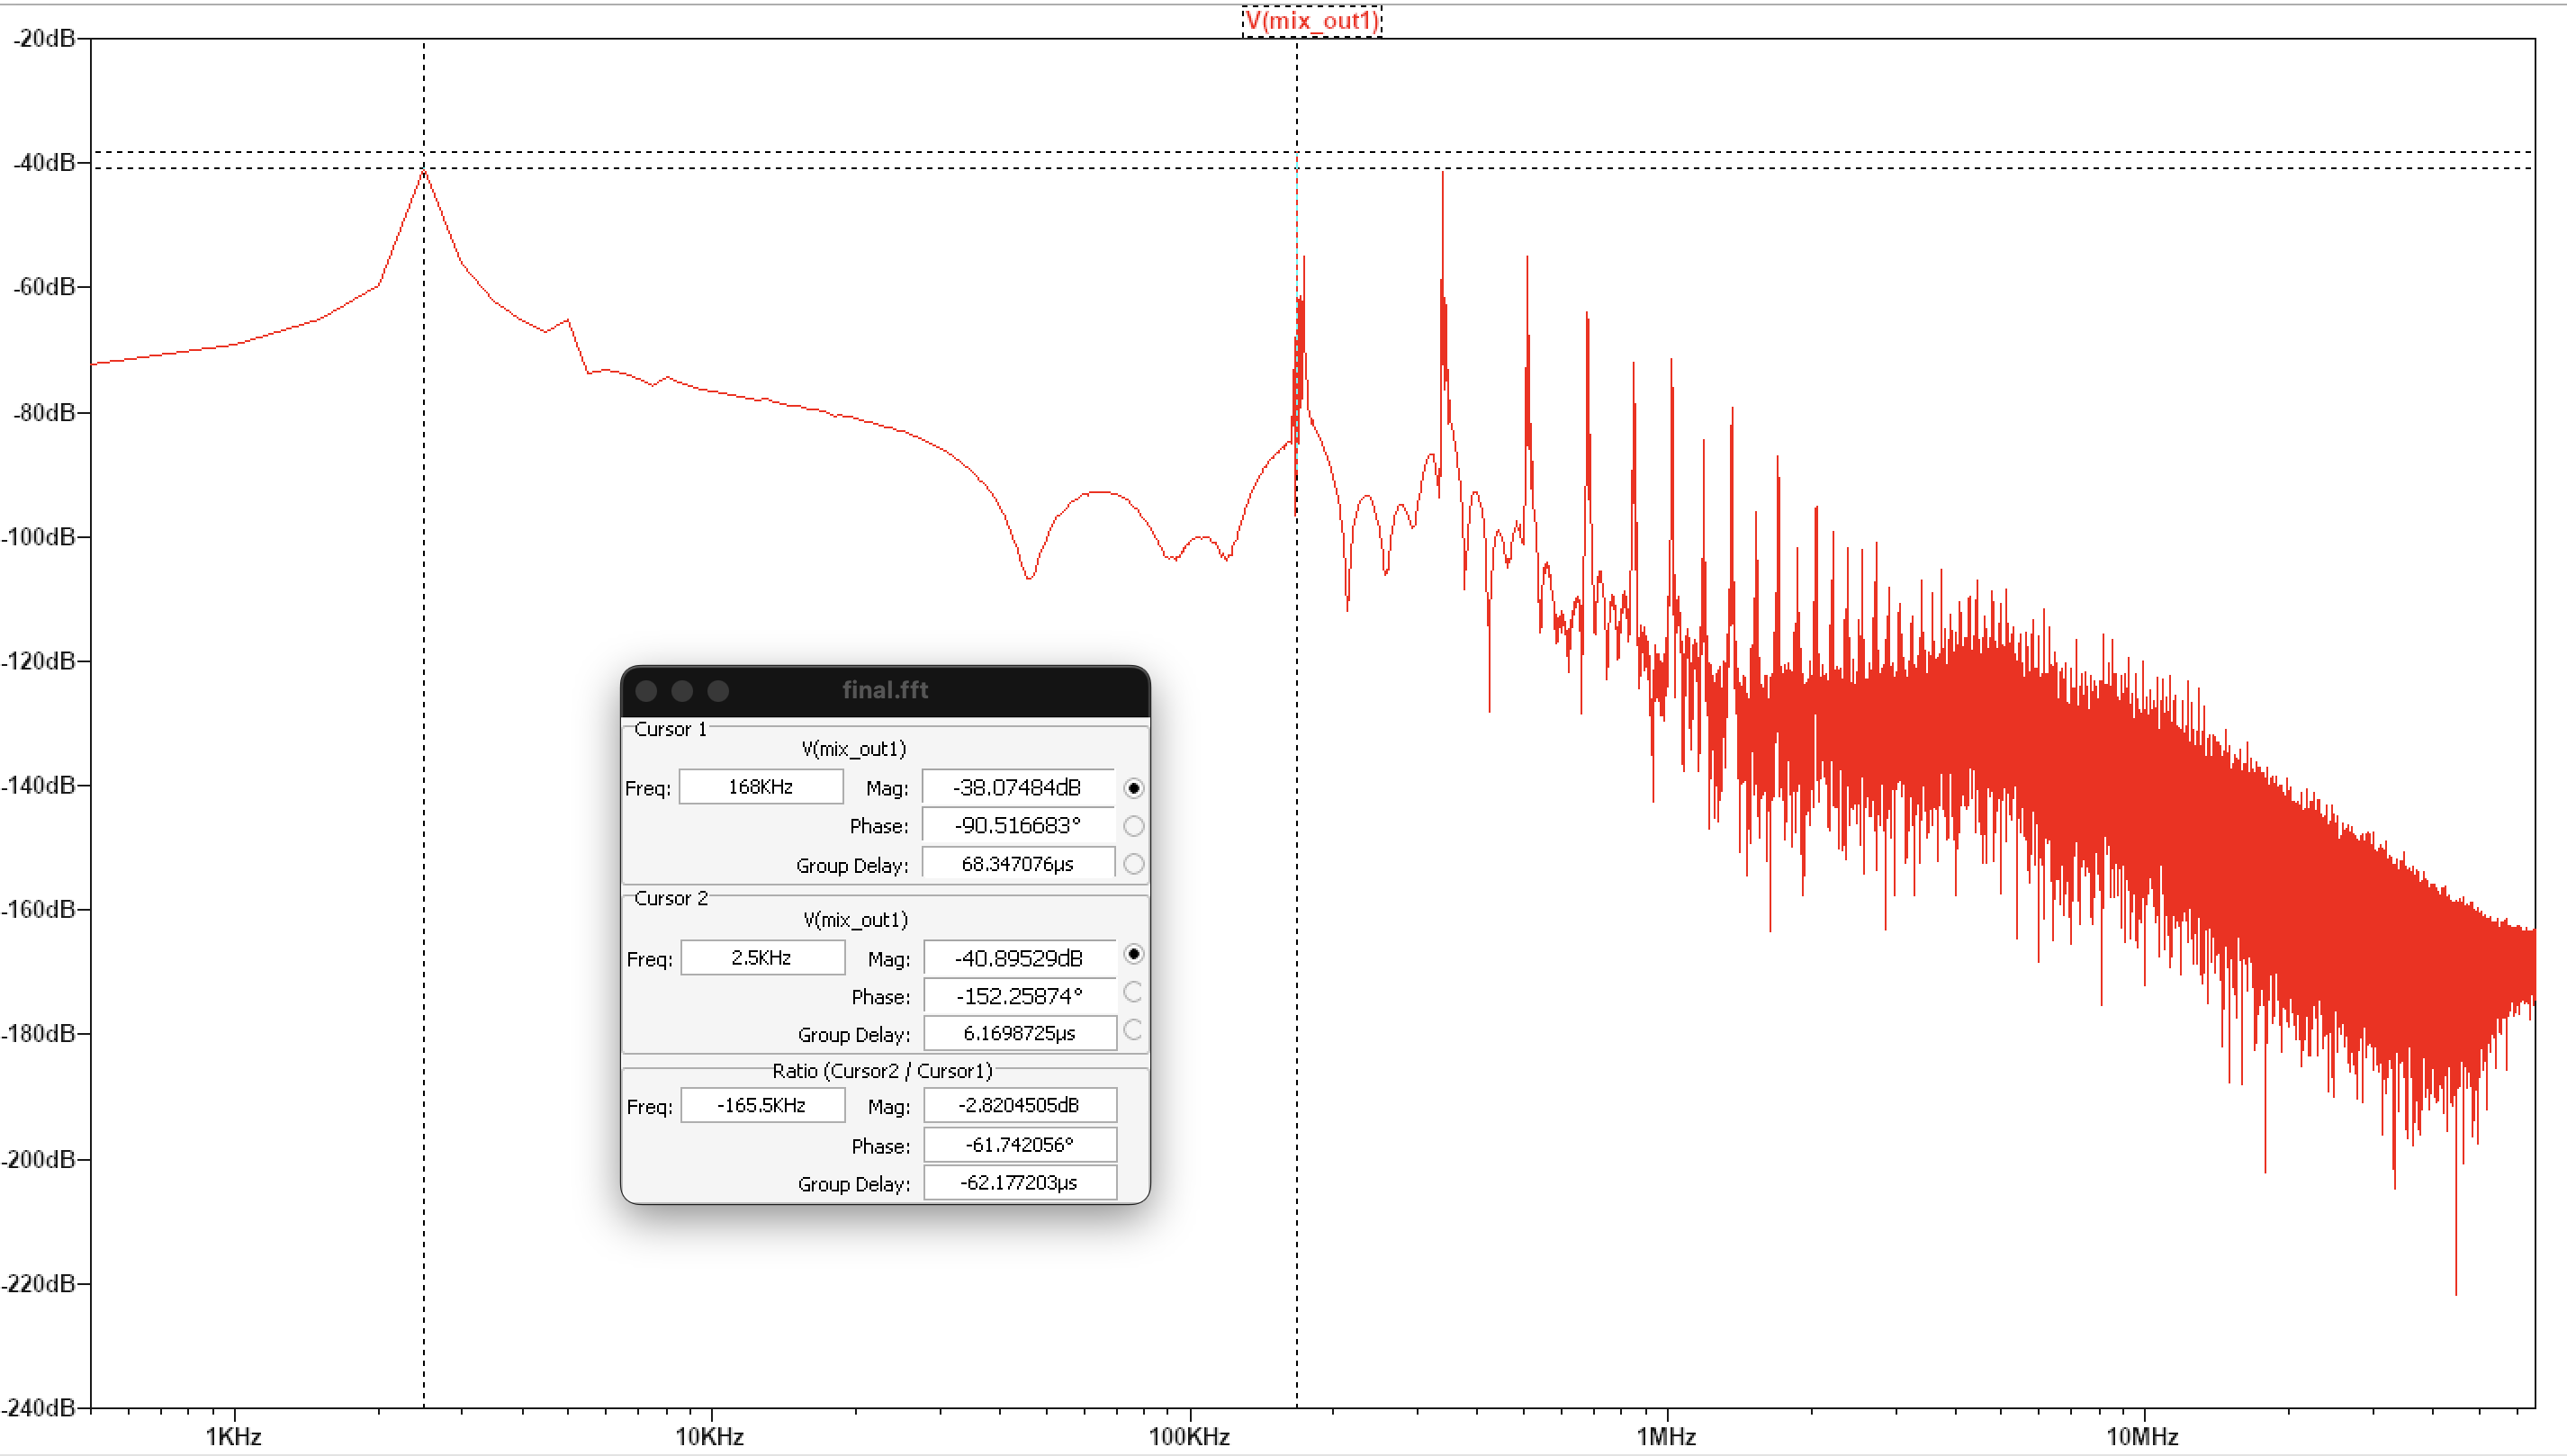
\includegraphics[width=\linewidth]{../report/images/168k-fft.png}
      \vspace{0.05cm}
      \tiny \textbf{$168\text{ kHz}$ Input:} $f_{\text{IF}} = 2\text{ kHz}$
    \end{column}
    \begin{column}{0.33\textwidth}
      \centering
      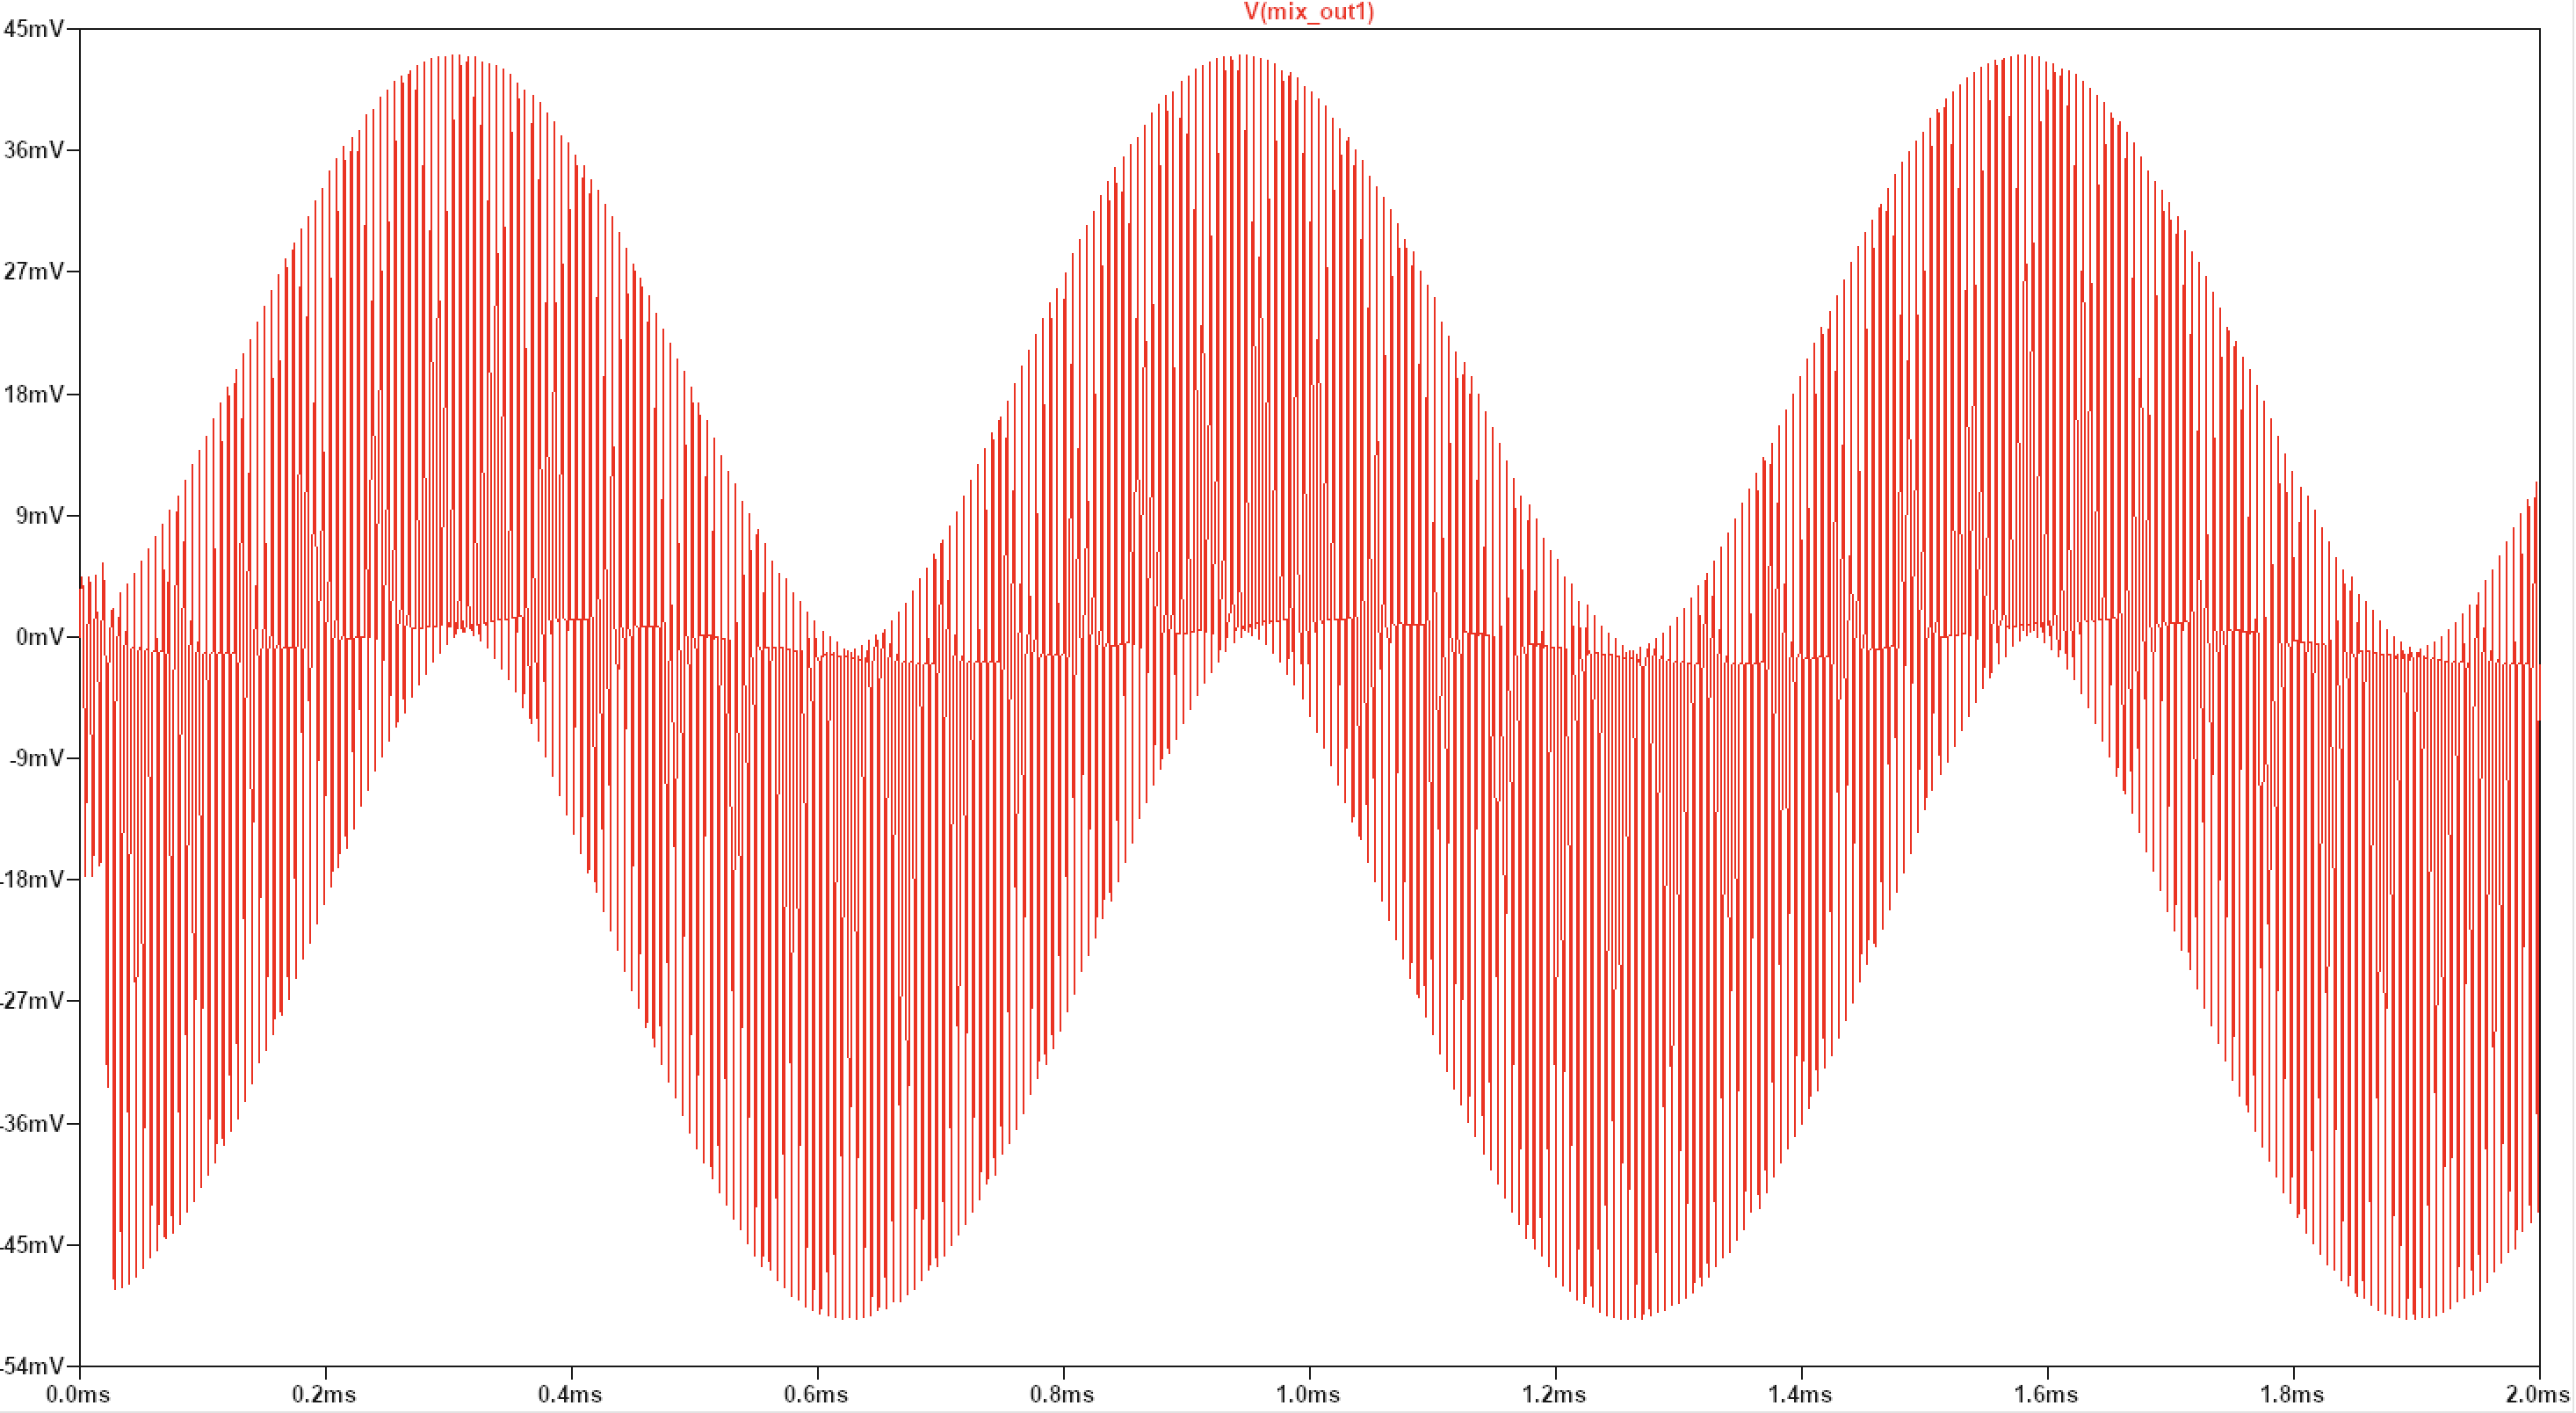
\includegraphics[width=\linewidth]{../report/images/169k-t.png} \\
      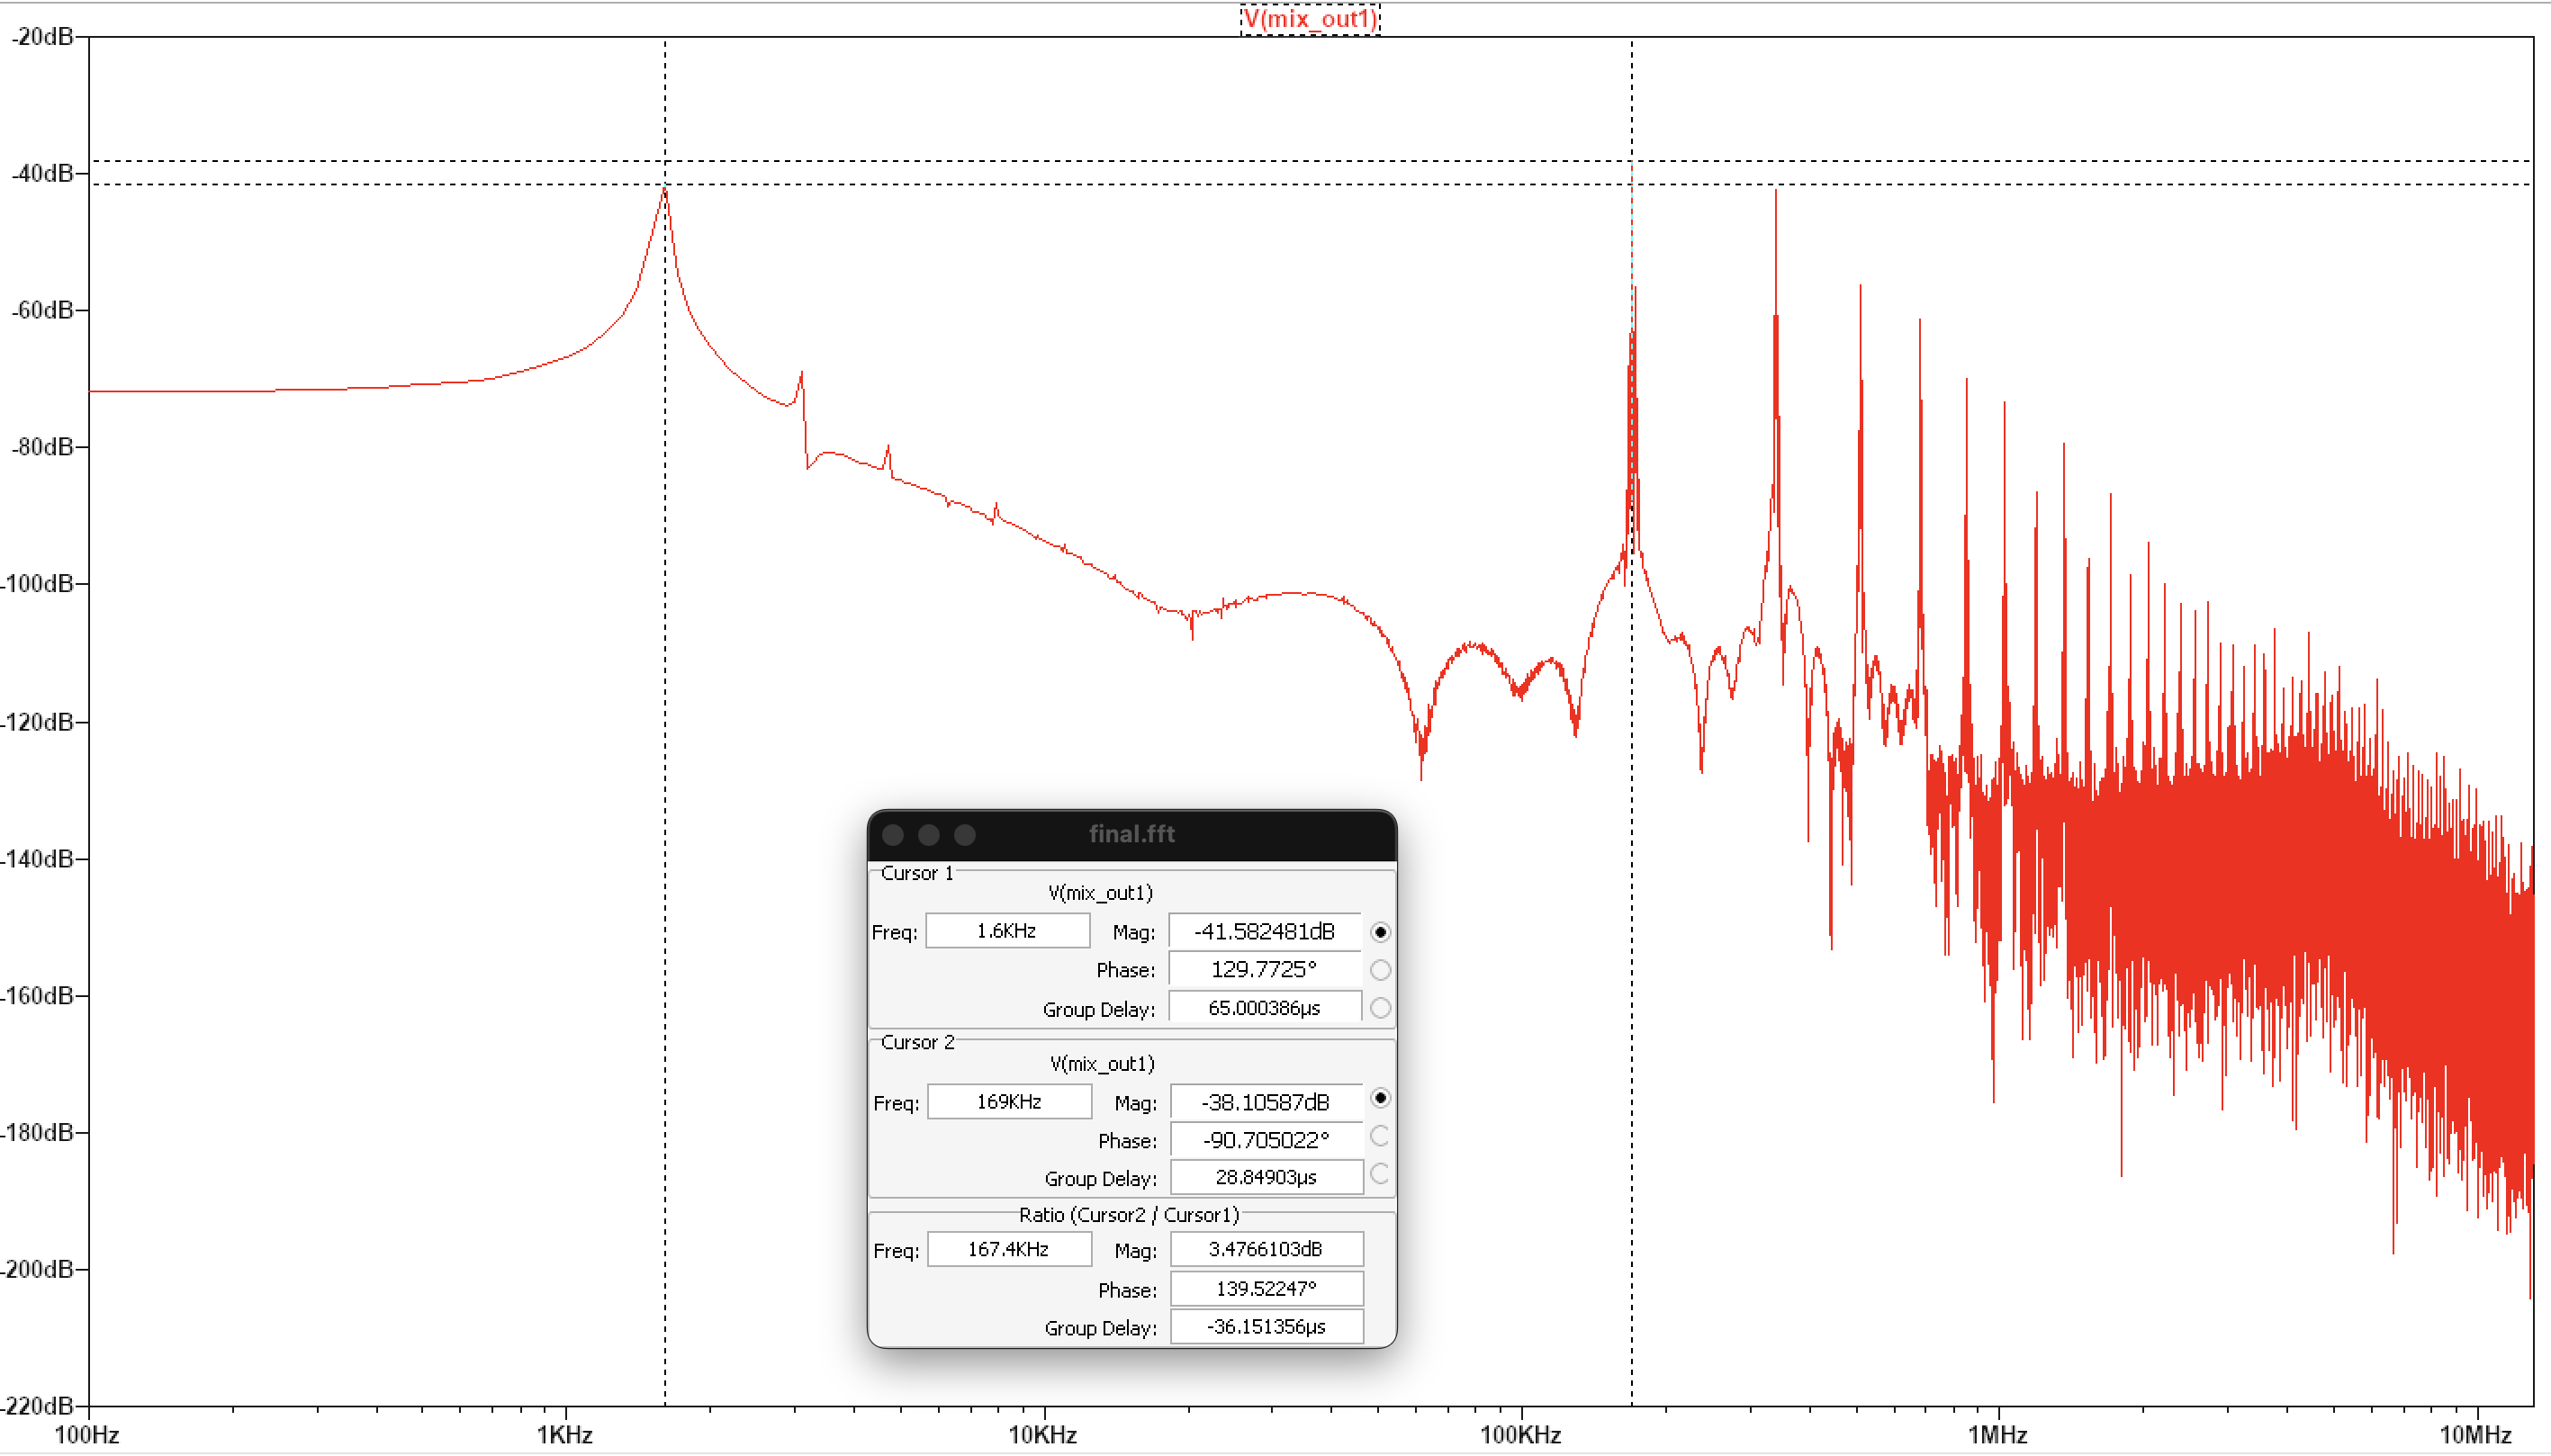
\includegraphics[width=\linewidth]{../report/images/169k-fft.png}
      \vspace{0.05cm}
      \tiny \textbf{$169\text{ kHz}$ Input:} $f_{\text{IF}} = 1\text{ kHz}$
    \end{column}
  \end{columns}
\end{frame}

% Slide 16: Mixer Frequency Sweep Analysis (171 kHz - 175 kHz)
\begin{frame}{Frequency Sweep Analysis ($f_{\text{IN}} > f_{\text{OSC}}$: 171--175 kHz)}
  \begin{columns}
    \begin{column}{0.33\textwidth}
      \centering
      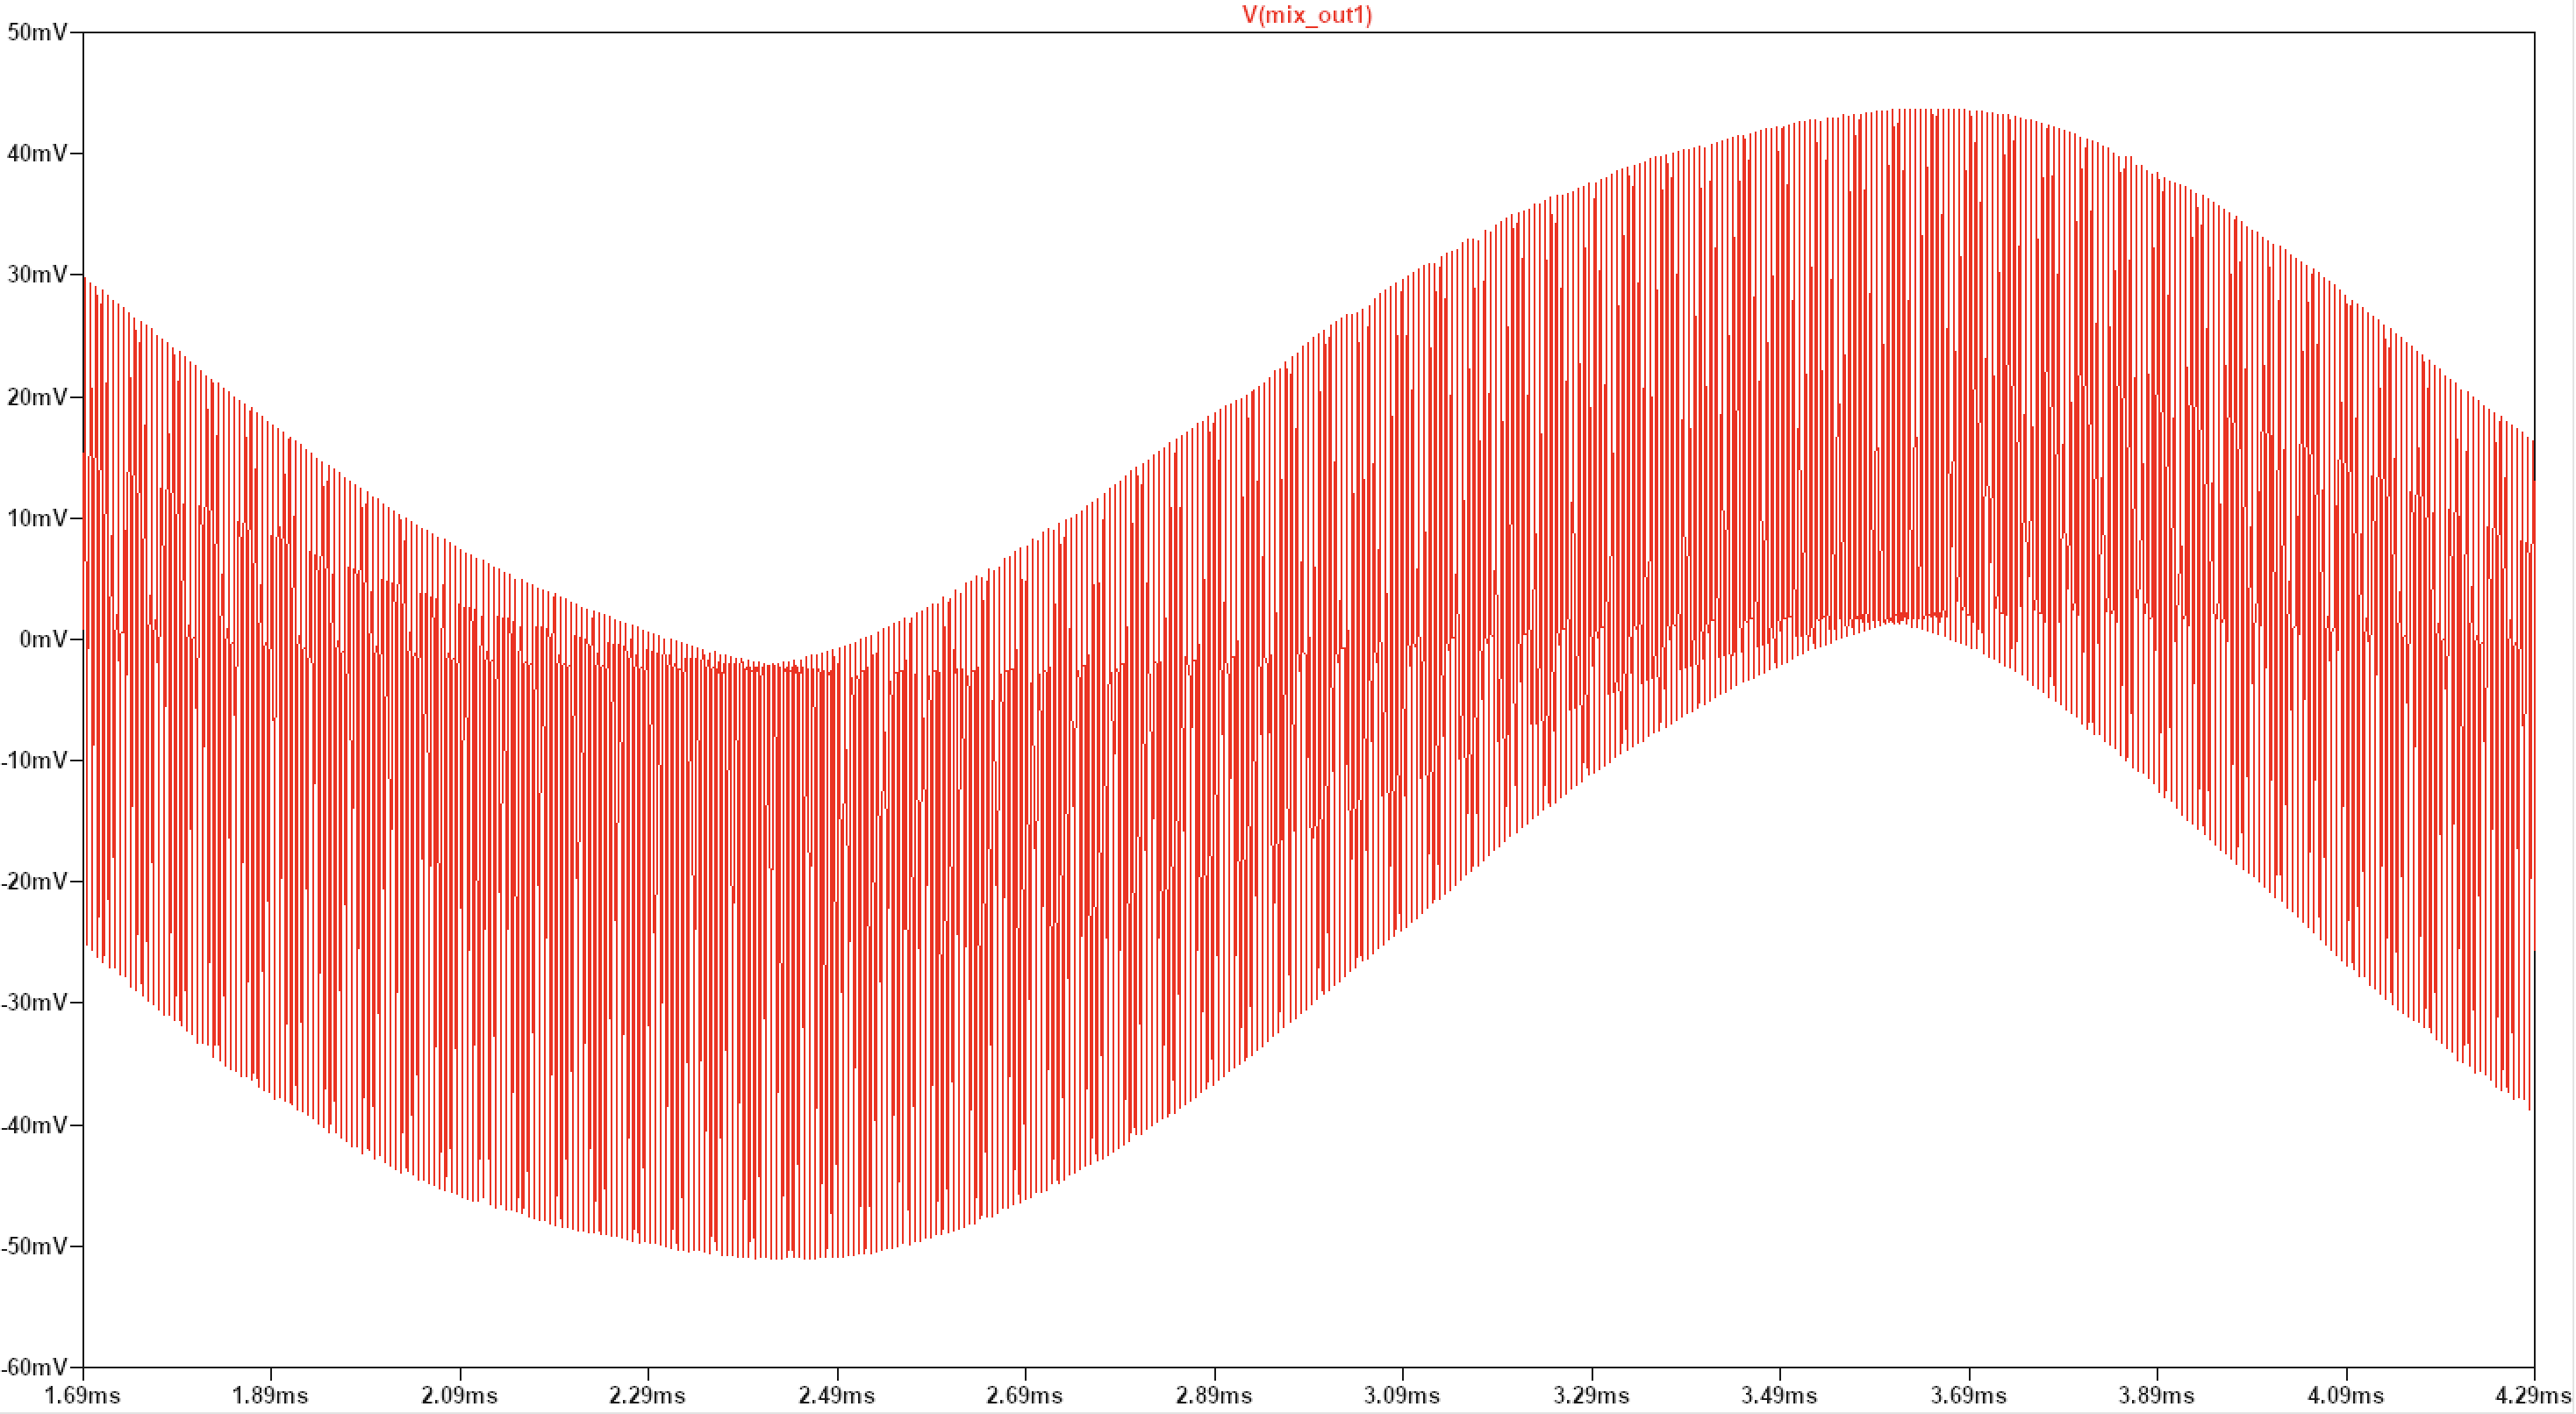
\includegraphics[width=\linewidth]{../report/images/171k-t.png} \\
      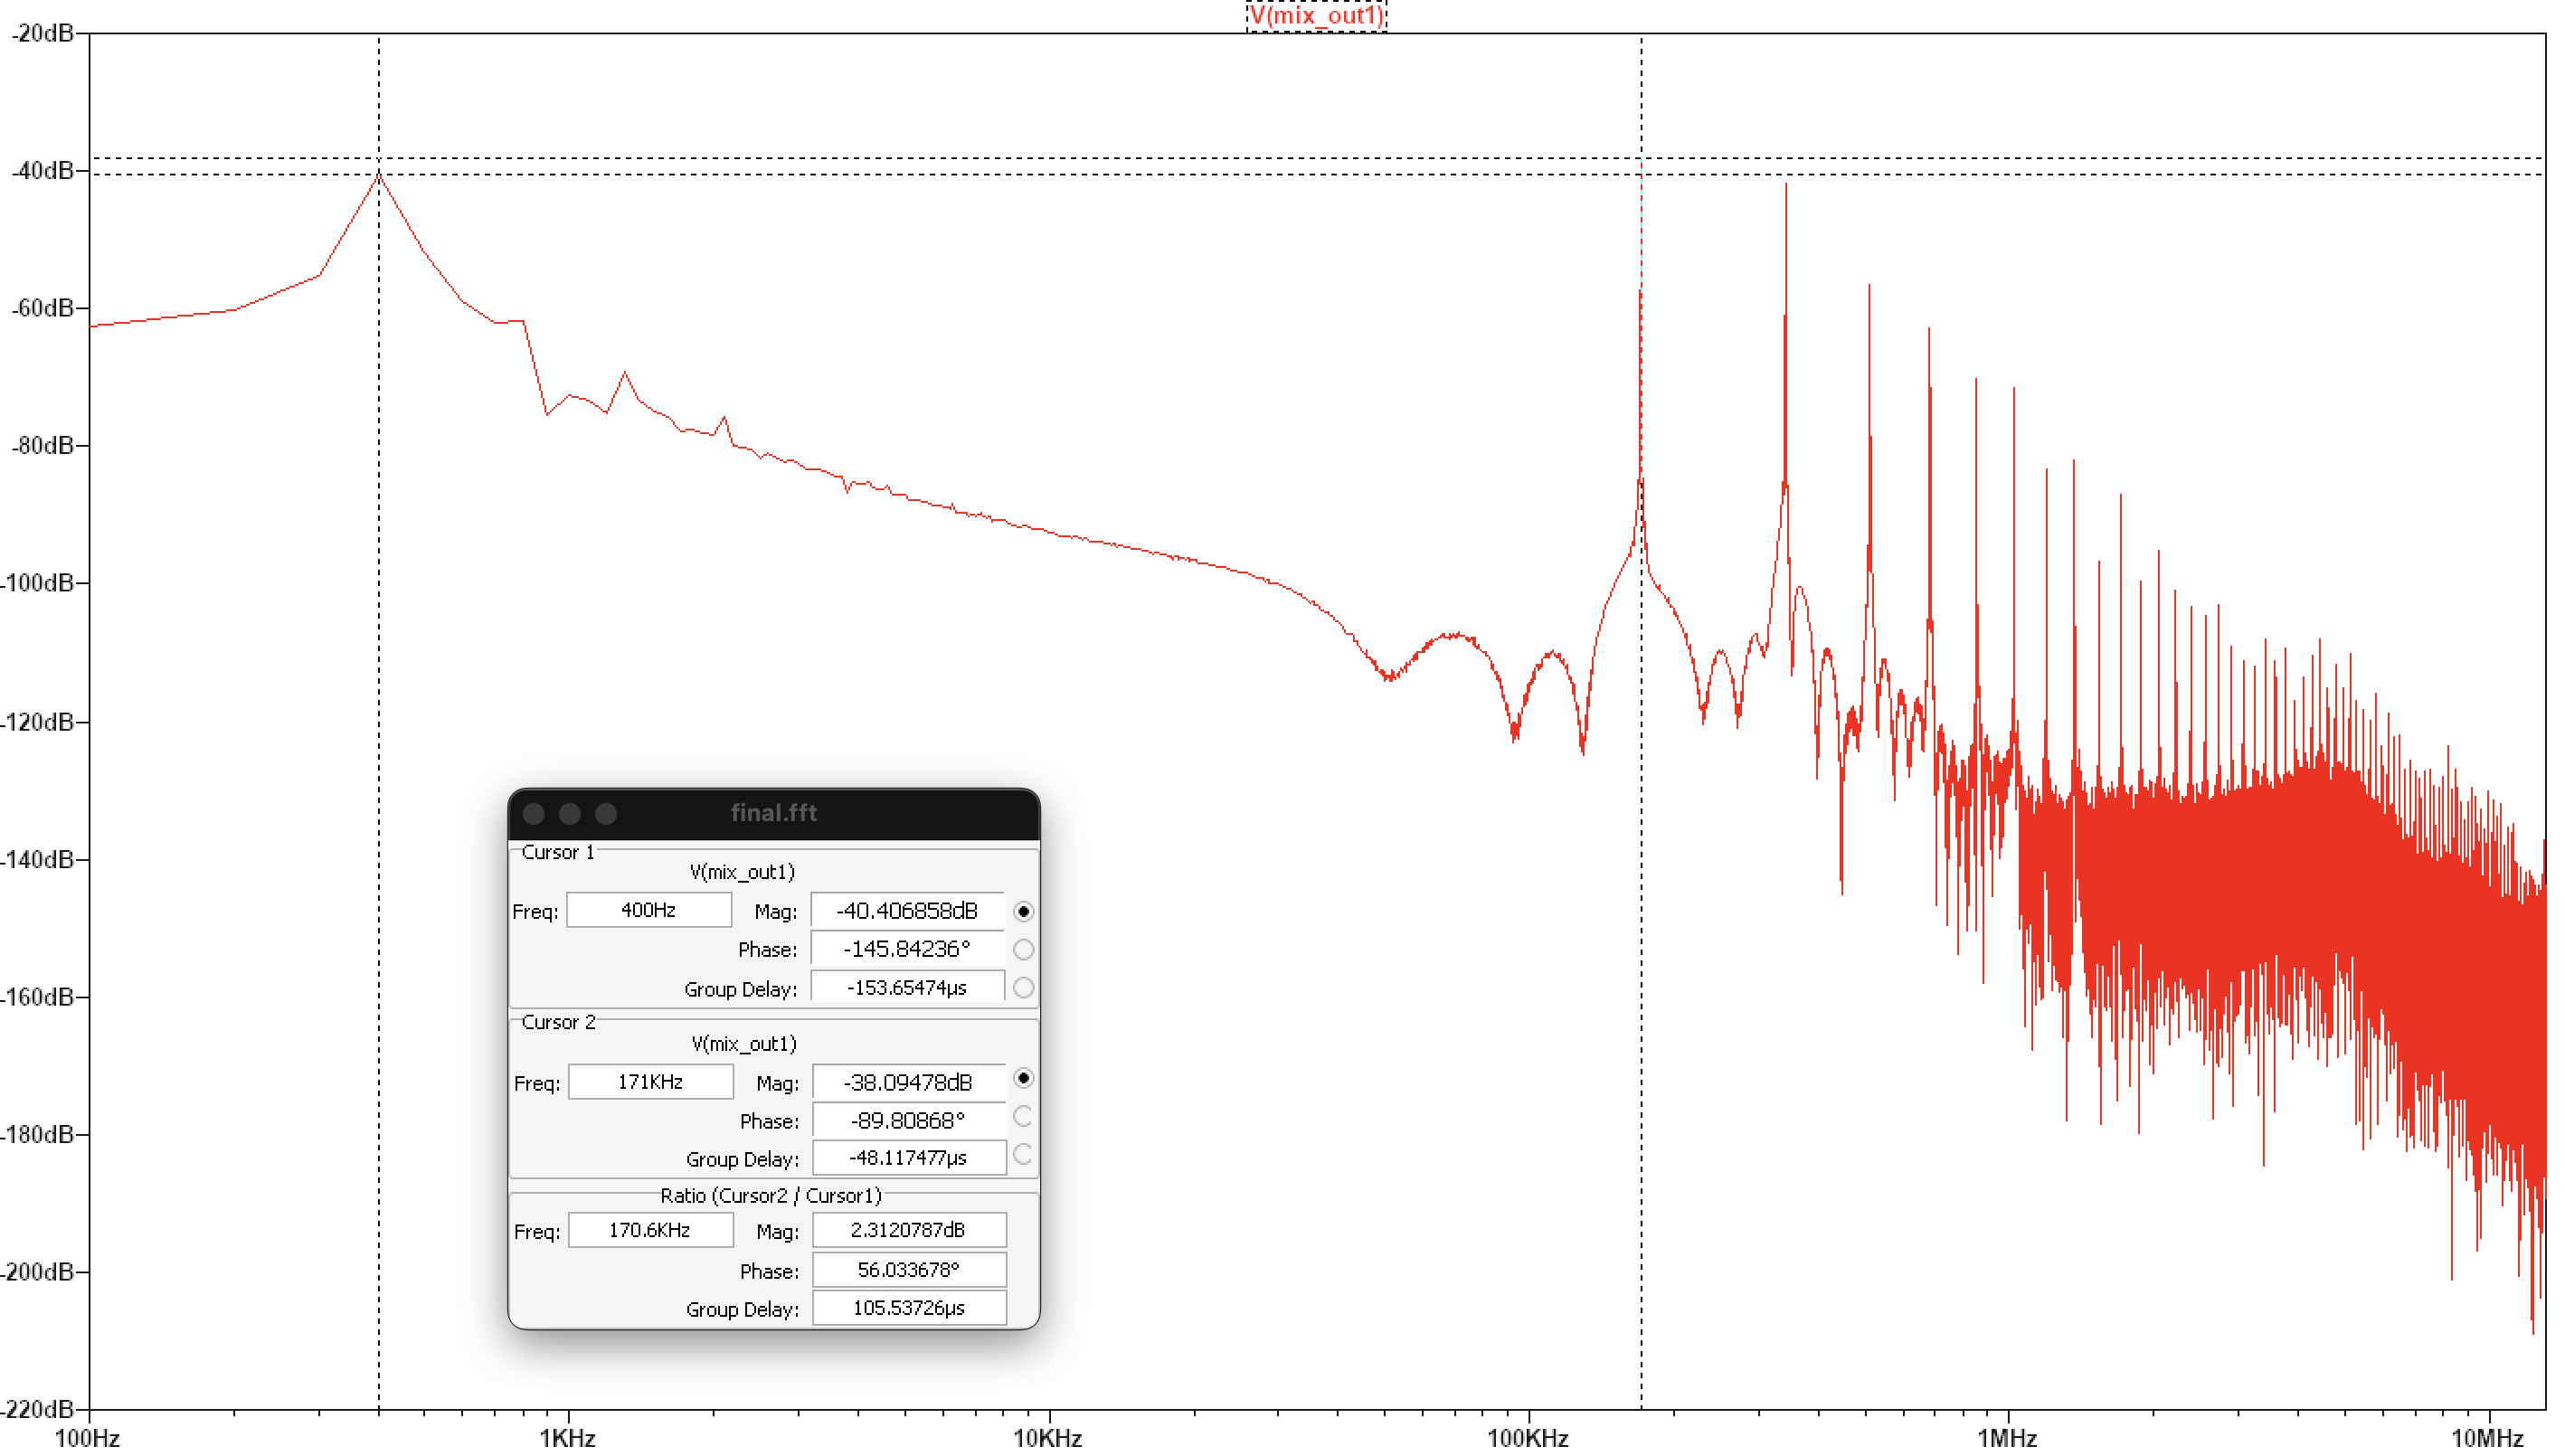
\includegraphics[width=\linewidth]{../report/images/171k-fft.png}
      \vspace{0.05cm}
      \tiny \textbf{$171\text{ kHz}$ Input:} $f_{\text{IF}} = 1\text{ kHz}$
    \end{column}
    \begin{column}{0.33\textwidth}
      \centering
      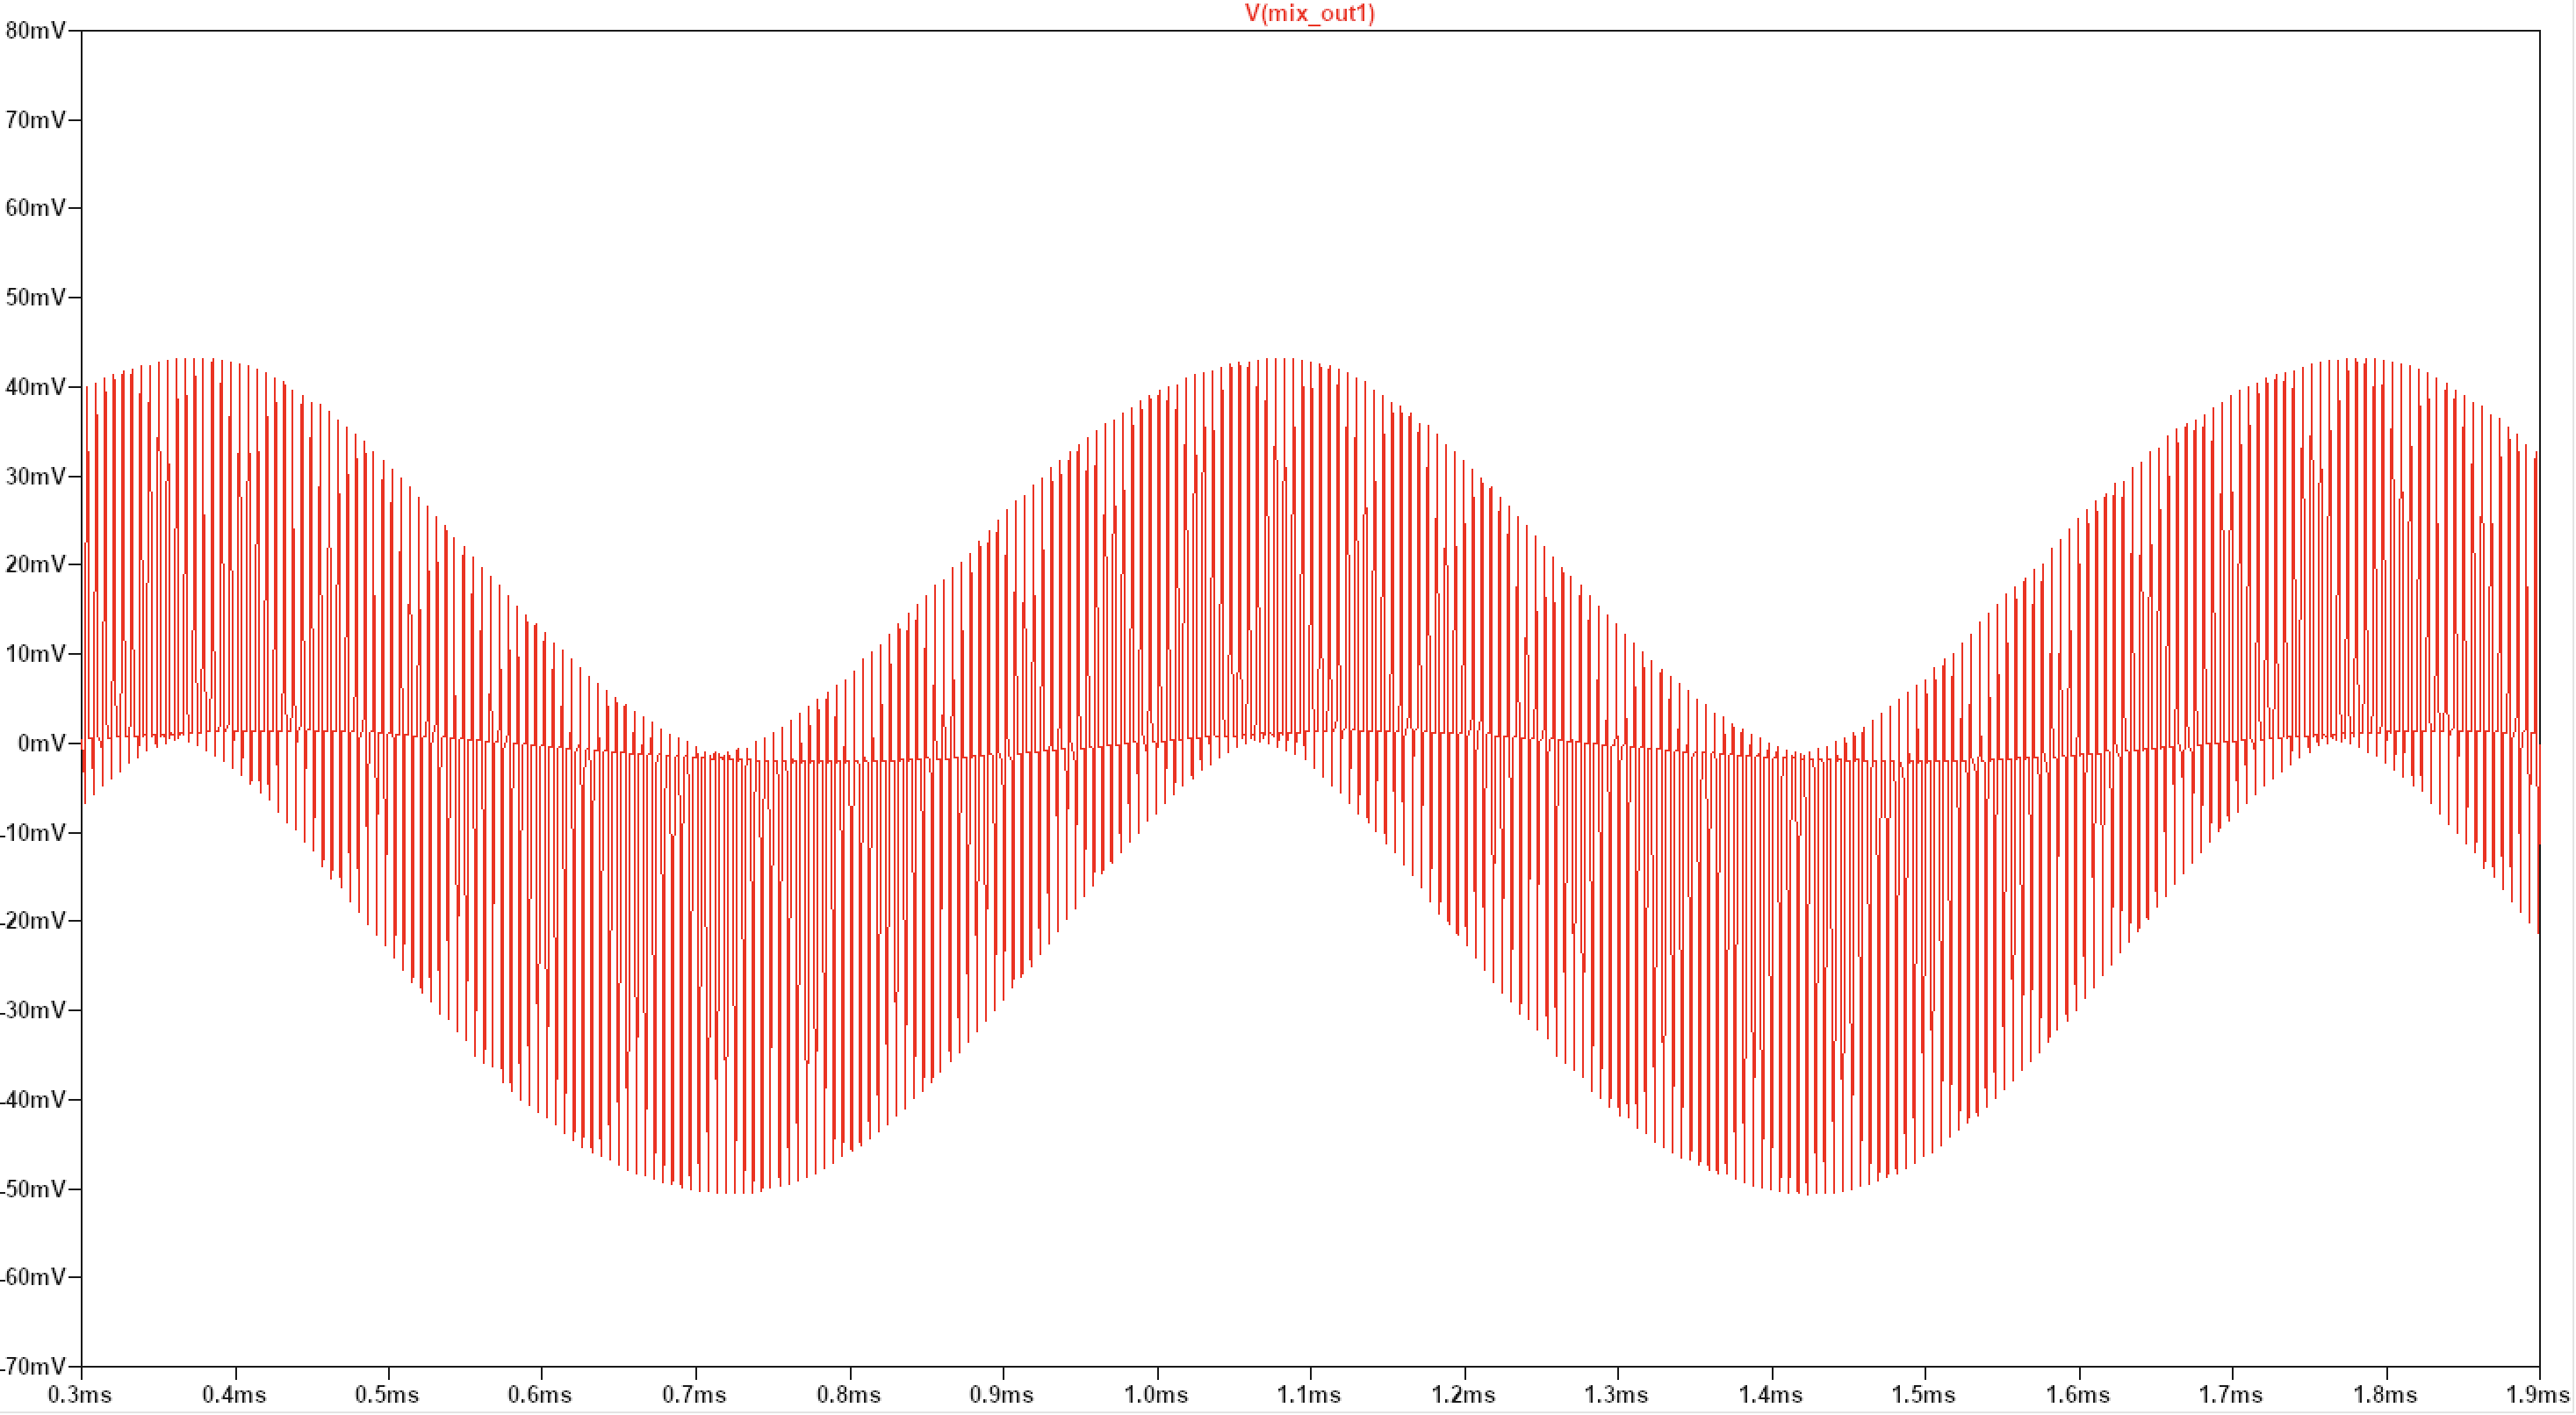
\includegraphics[width=\linewidth]{../report/images/172k-t.png} \\
      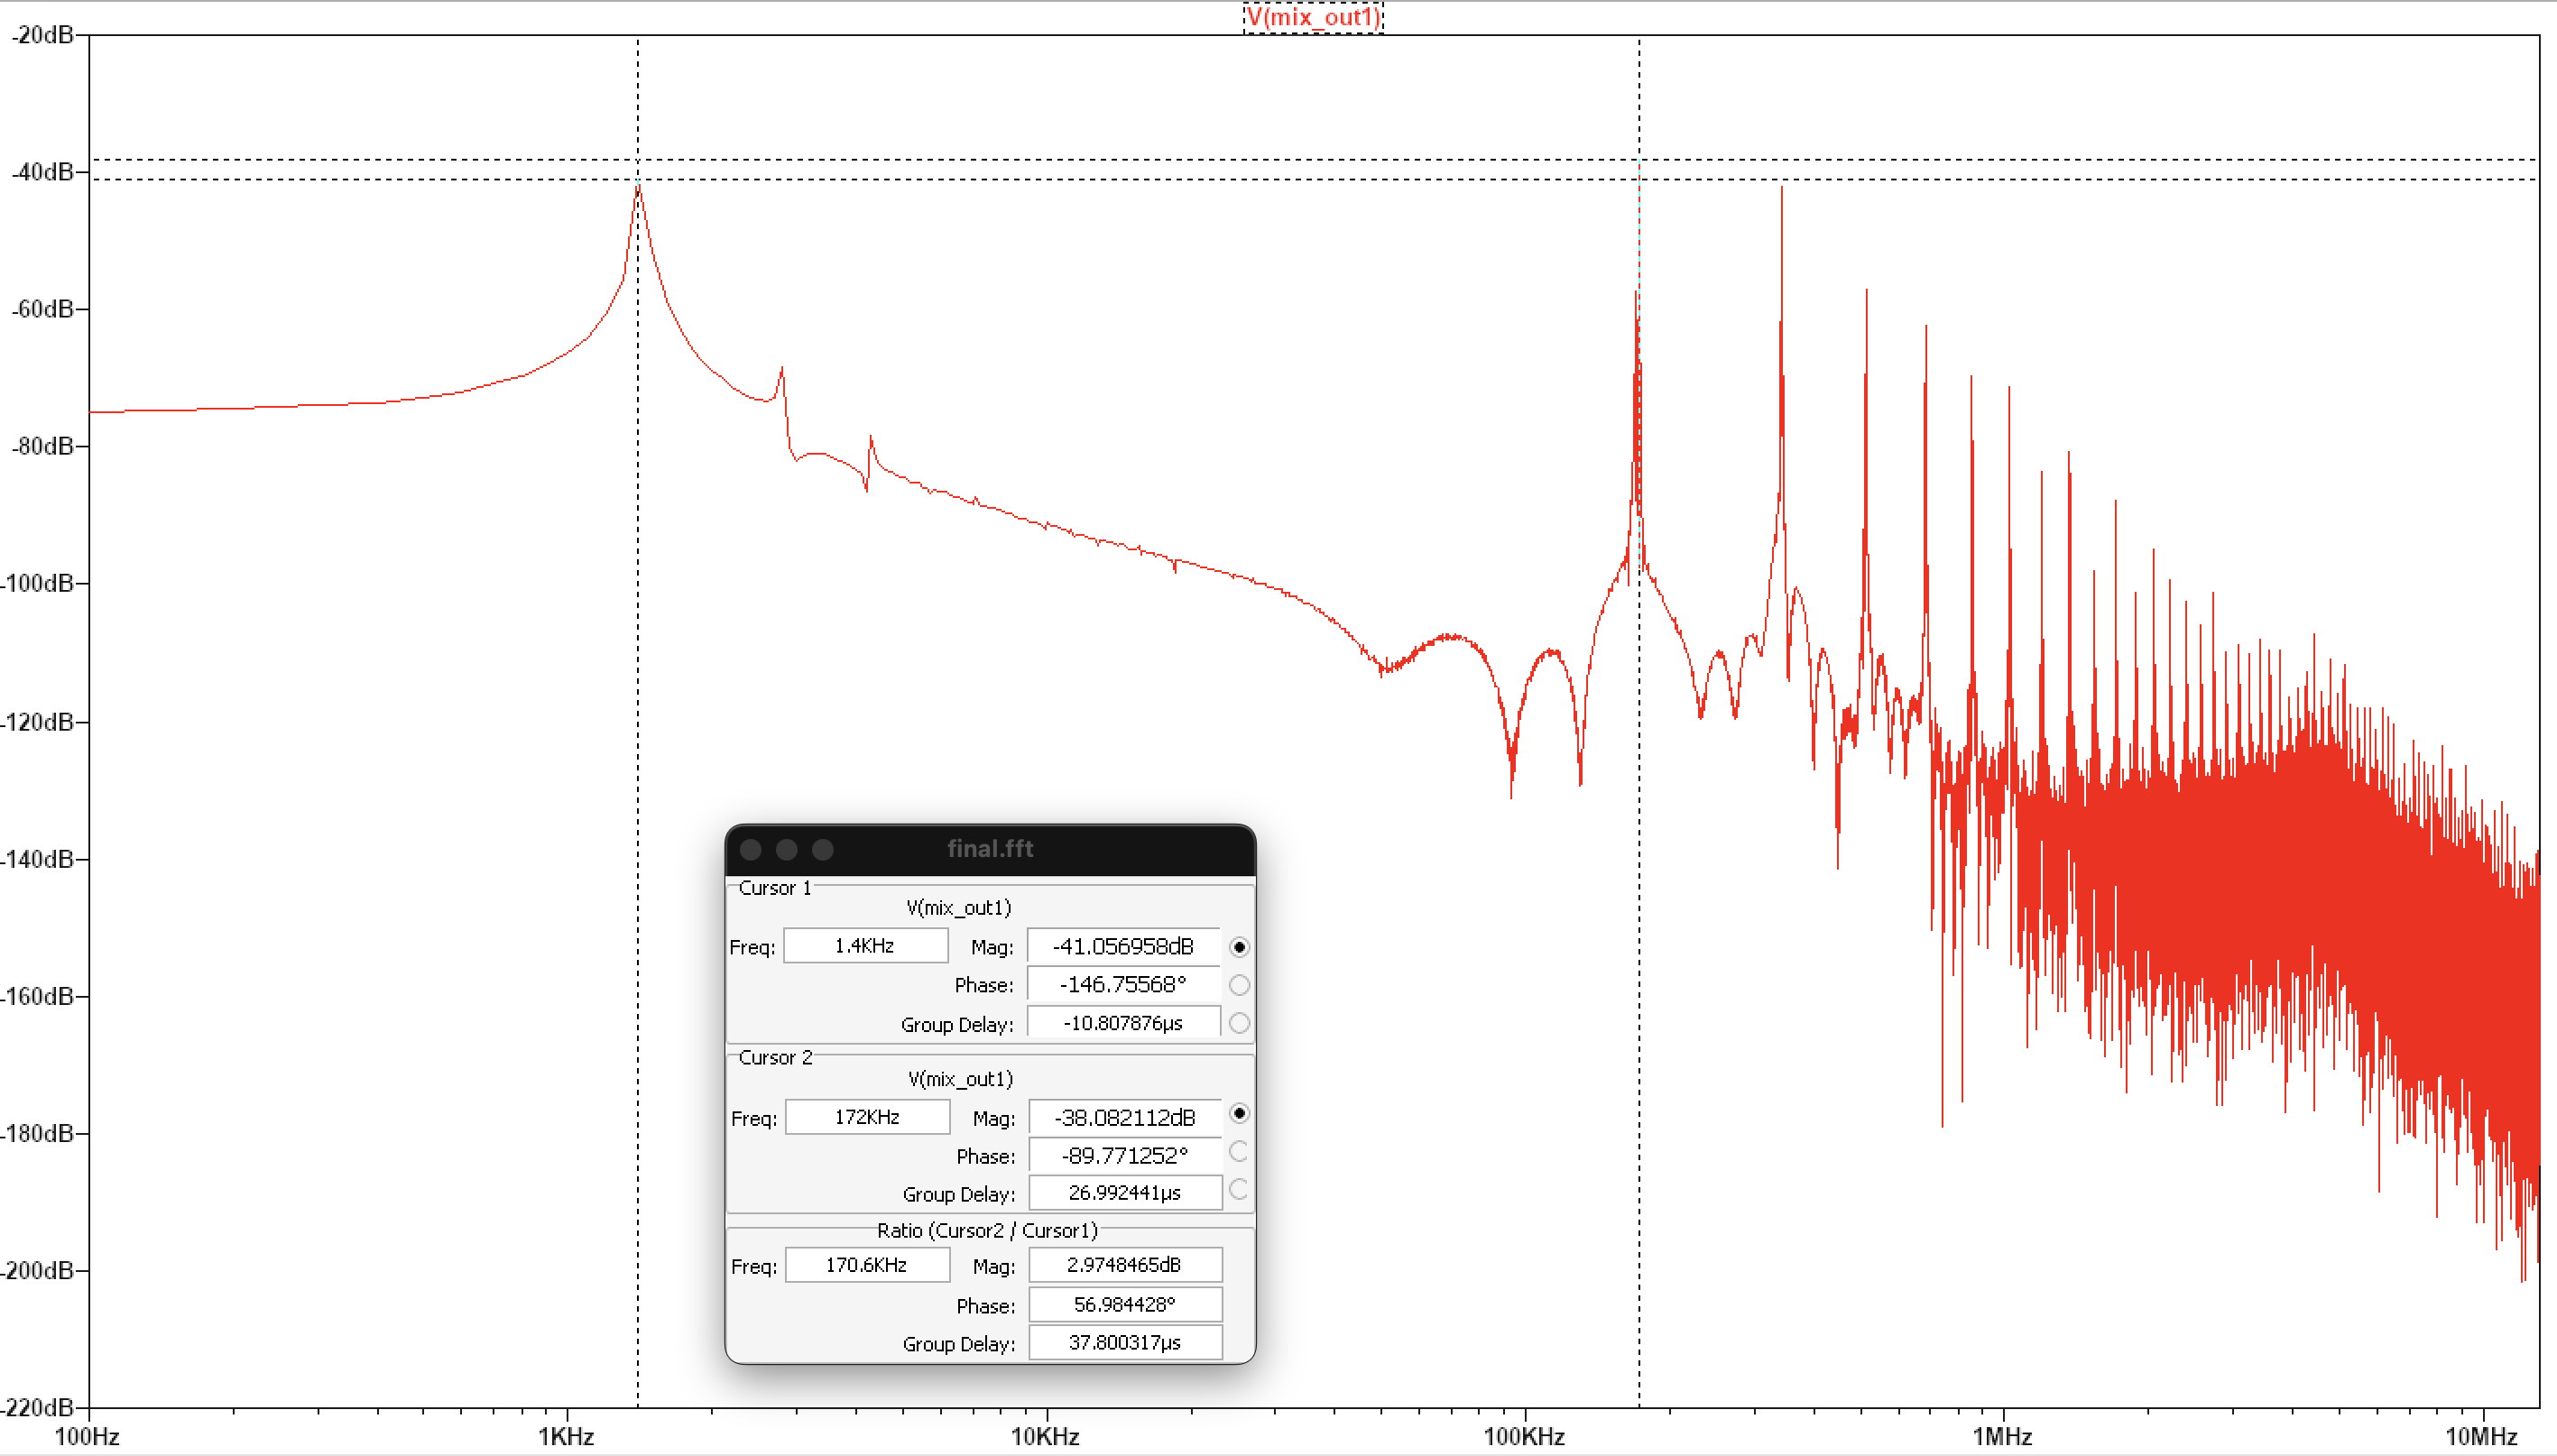
\includegraphics[width=\linewidth]{../report/images/172k-fft.png}
      \vspace{0.05cm}
      \tiny \textbf{$172\text{ kHz}$ Input:} $f_{\text{IF}} = 2\text{ kHz}$
    \end{column}
    \begin{column}{0.33\textwidth}
      \centering
      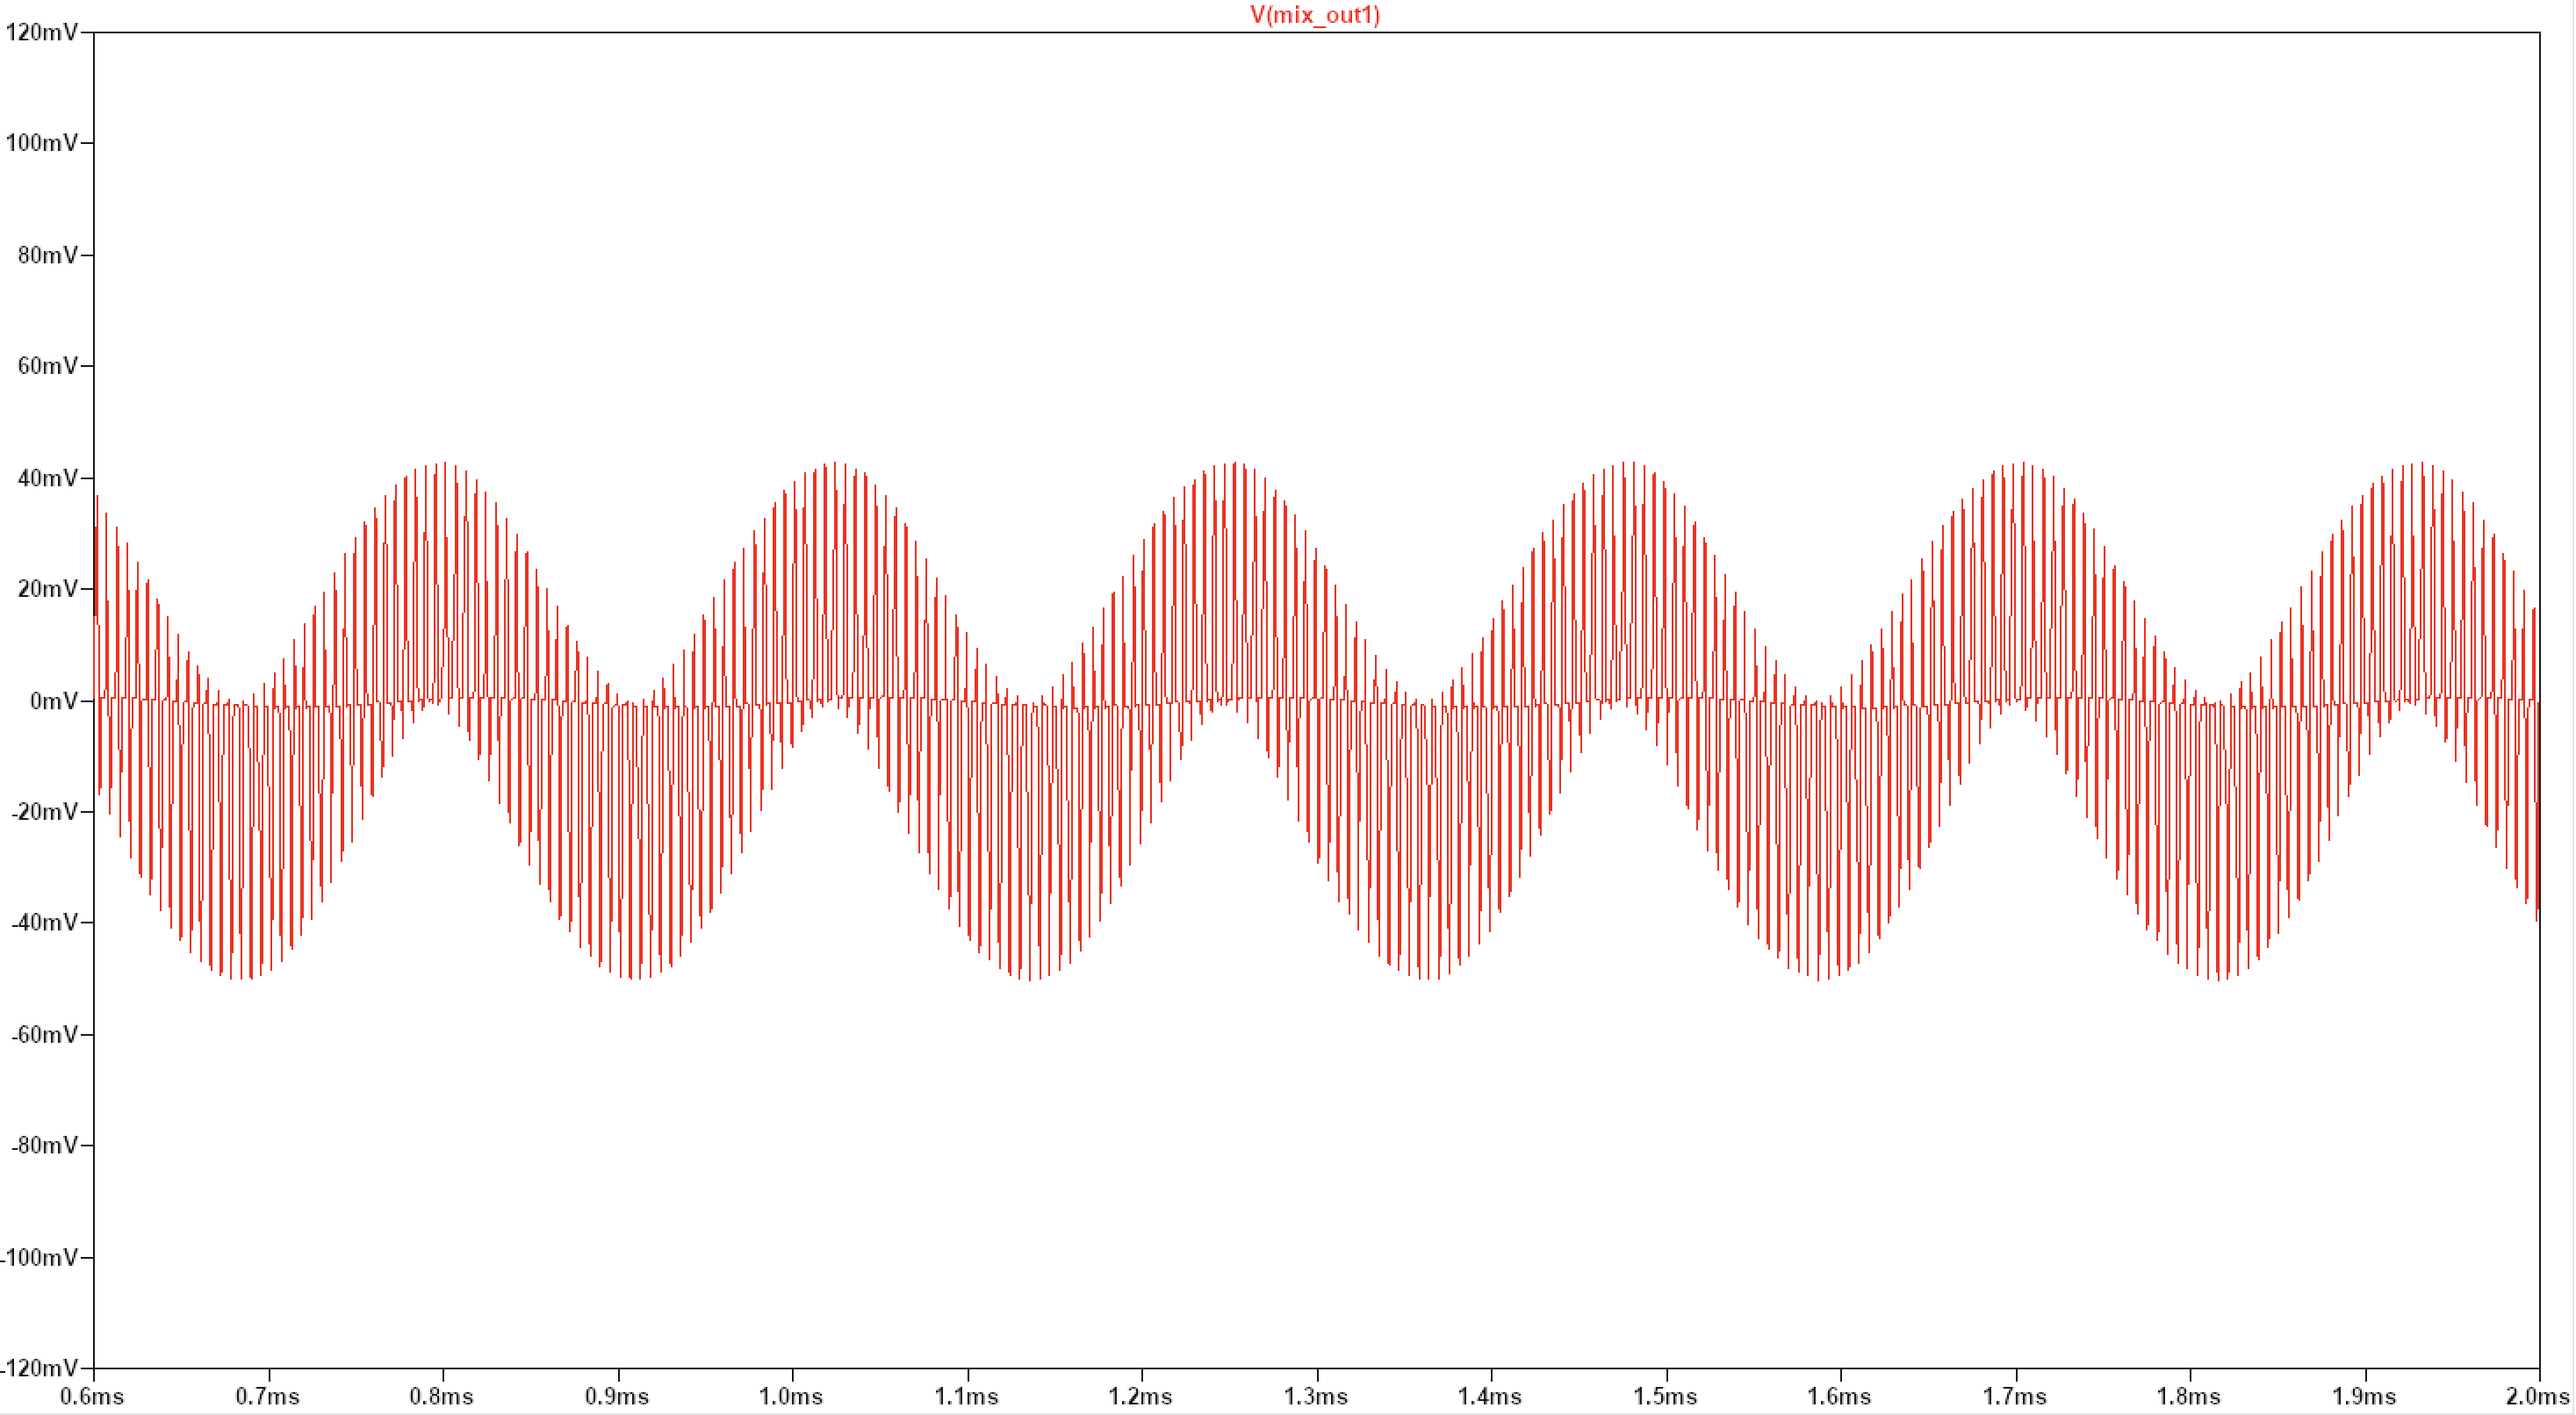
\includegraphics[width=\linewidth]{../report/images/175k-t.png} \\
      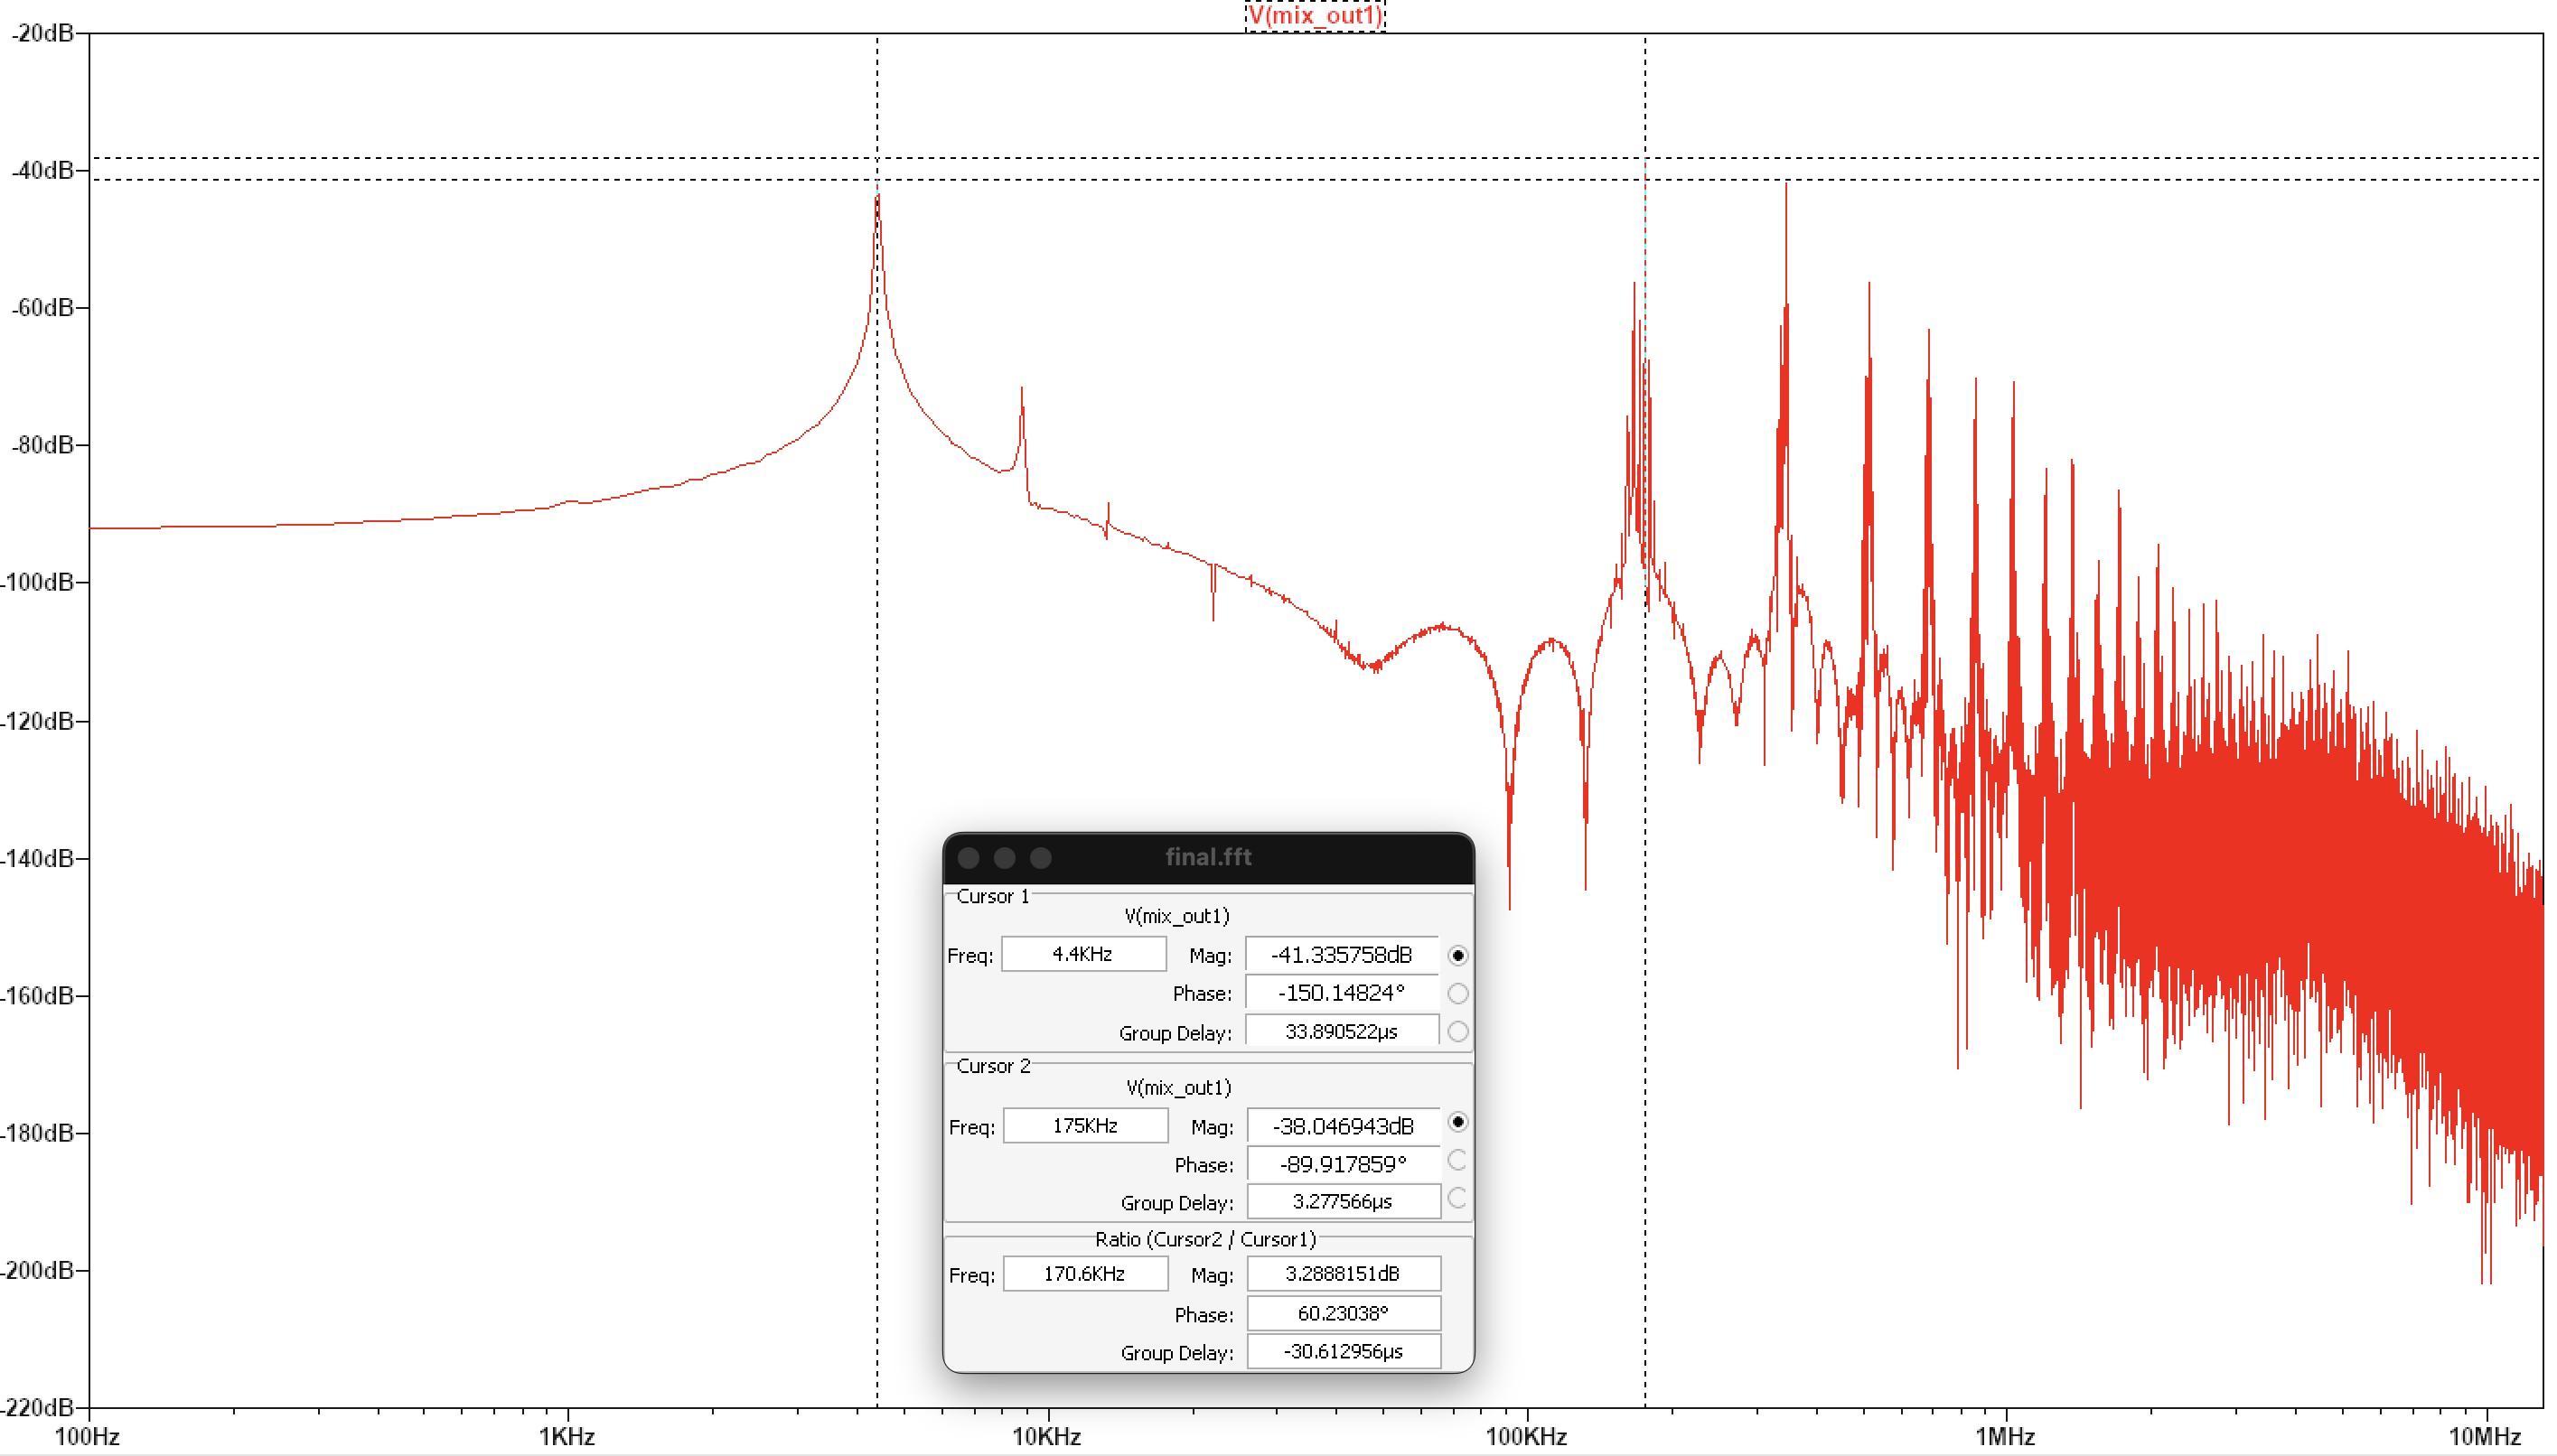
\includegraphics[width=\linewidth]{../report/images/175k-fft.png}
      \vspace{0.05cm}
      \tiny \textbf{$175\text{ kHz}$ Input:} $f_{\text{IF}} = 5\text{ kHz}$
    \end{column}
  \end{columns}
\end{frame}

% Slide 17: Hardware Realization & DSO Measurements
\begin{frame}{Mixer Lab Realization \& DSO Waveform Captures}
  \begin{columns}
    \begin{column}{0.5\textwidth}
      \centering
      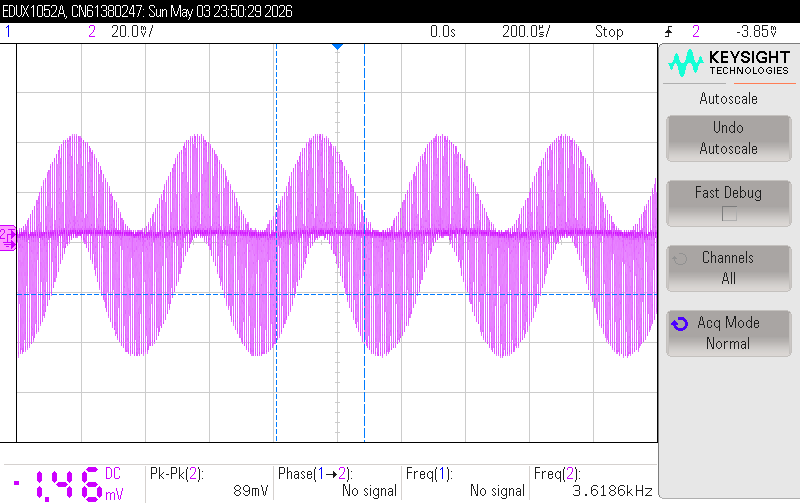
\includegraphics[width=\linewidth]{../report/images/mixer-img1.png}
      \vspace{0.1cm}
      \tiny DSO Measurement 1: Hardware NMOS mixer output envelope.
    \end{column}
    \begin{column}{0.5\textwidth}
      \centering
      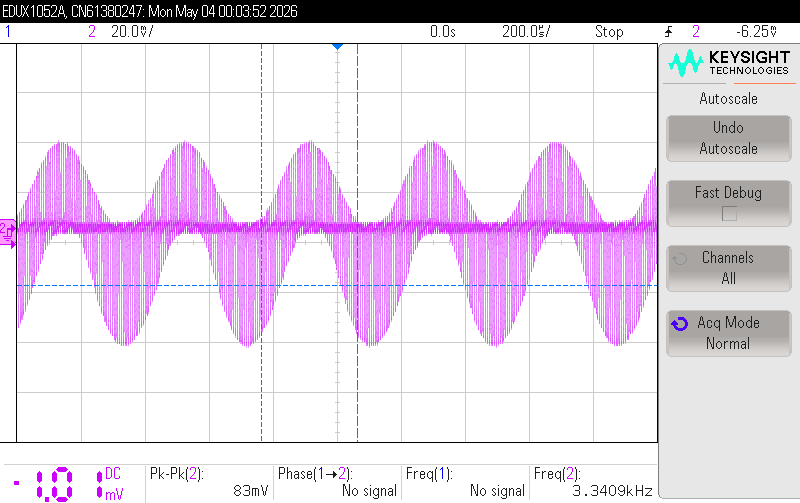
\includegraphics[width=\linewidth]{../report/images/mixer-img2.png}
      \vspace{0.1cm}
      \tiny DSO Measurement 2: High-frequency carrier with low-frequency IF envelope.
    \end{column}
  \end{columns}
  \vspace{0.15cm}
  \scriptsize
  \textbf{Result:} Laboratory NMOS hardware confirms successful frequency downconversion matching SPICE predictions.
\end{frame}

\section{Low-Pass Filter \& Amplifier Design}

% Slide 18: First-Order Low-Pass Filter Calculations
\begin{frame}{Low-Pass RC Filter Design \& Cutoff Calculations}
  \begin{columns}
    \begin{column}{0.5\textwidth}
      \centering
      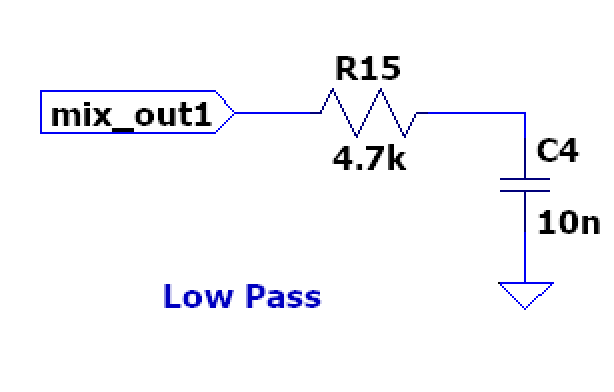
\includegraphics[width=0.85\linewidth]{../report/images/lowpass.png}
      \vspace{0.1cm}
      \tiny First-Order RC Low-Pass Filter Schematic.
    \end{column}
    \begin{column}{0.5\textwidth}
      \begin{itemize}
        \item \textbf{Cutoff Frequency Formula:}
        \begin{equation*}
          f_c = \frac{1}{2\pi RC}
        \end{equation*}
        \item \textbf{Lab Practical Implementation:}
        \begin{itemize}
          \item $R = 4.7\text{ k}\Omega$, $C = 10\text{ nF}$
          \item $f_c = \frac{1}{2\pi (4700)(10\,\text{n})} \approx \mathbf{3.39\text{ kHz}}$
        \end{itemize}
        \item \textbf{Theoretical $3\text{ kHz}$ Target Resistor:}
        \begin{align*}
          R_{\text{ideal}} &= \frac{1}{2\pi (3000)(10\,\text{nF})} \\
                           &\approx \mathbf{5.3\text{ k}\Omega}
        \end{align*}
      \end{itemize}
    \end{column}
  \end{columns}
\end{frame}

% Slide 19: Single-Stage vs. Two-Stage Cascaded LPF
\begin{frame}{LPF Optimization -- 1-Stage vs. 2-Stage Cascaded LPF}
  \begin{columns}
    \begin{column}{0.5\textwidth}
      \begin{block}{Iteration 1: Single-Stage LPF}
        \centering
        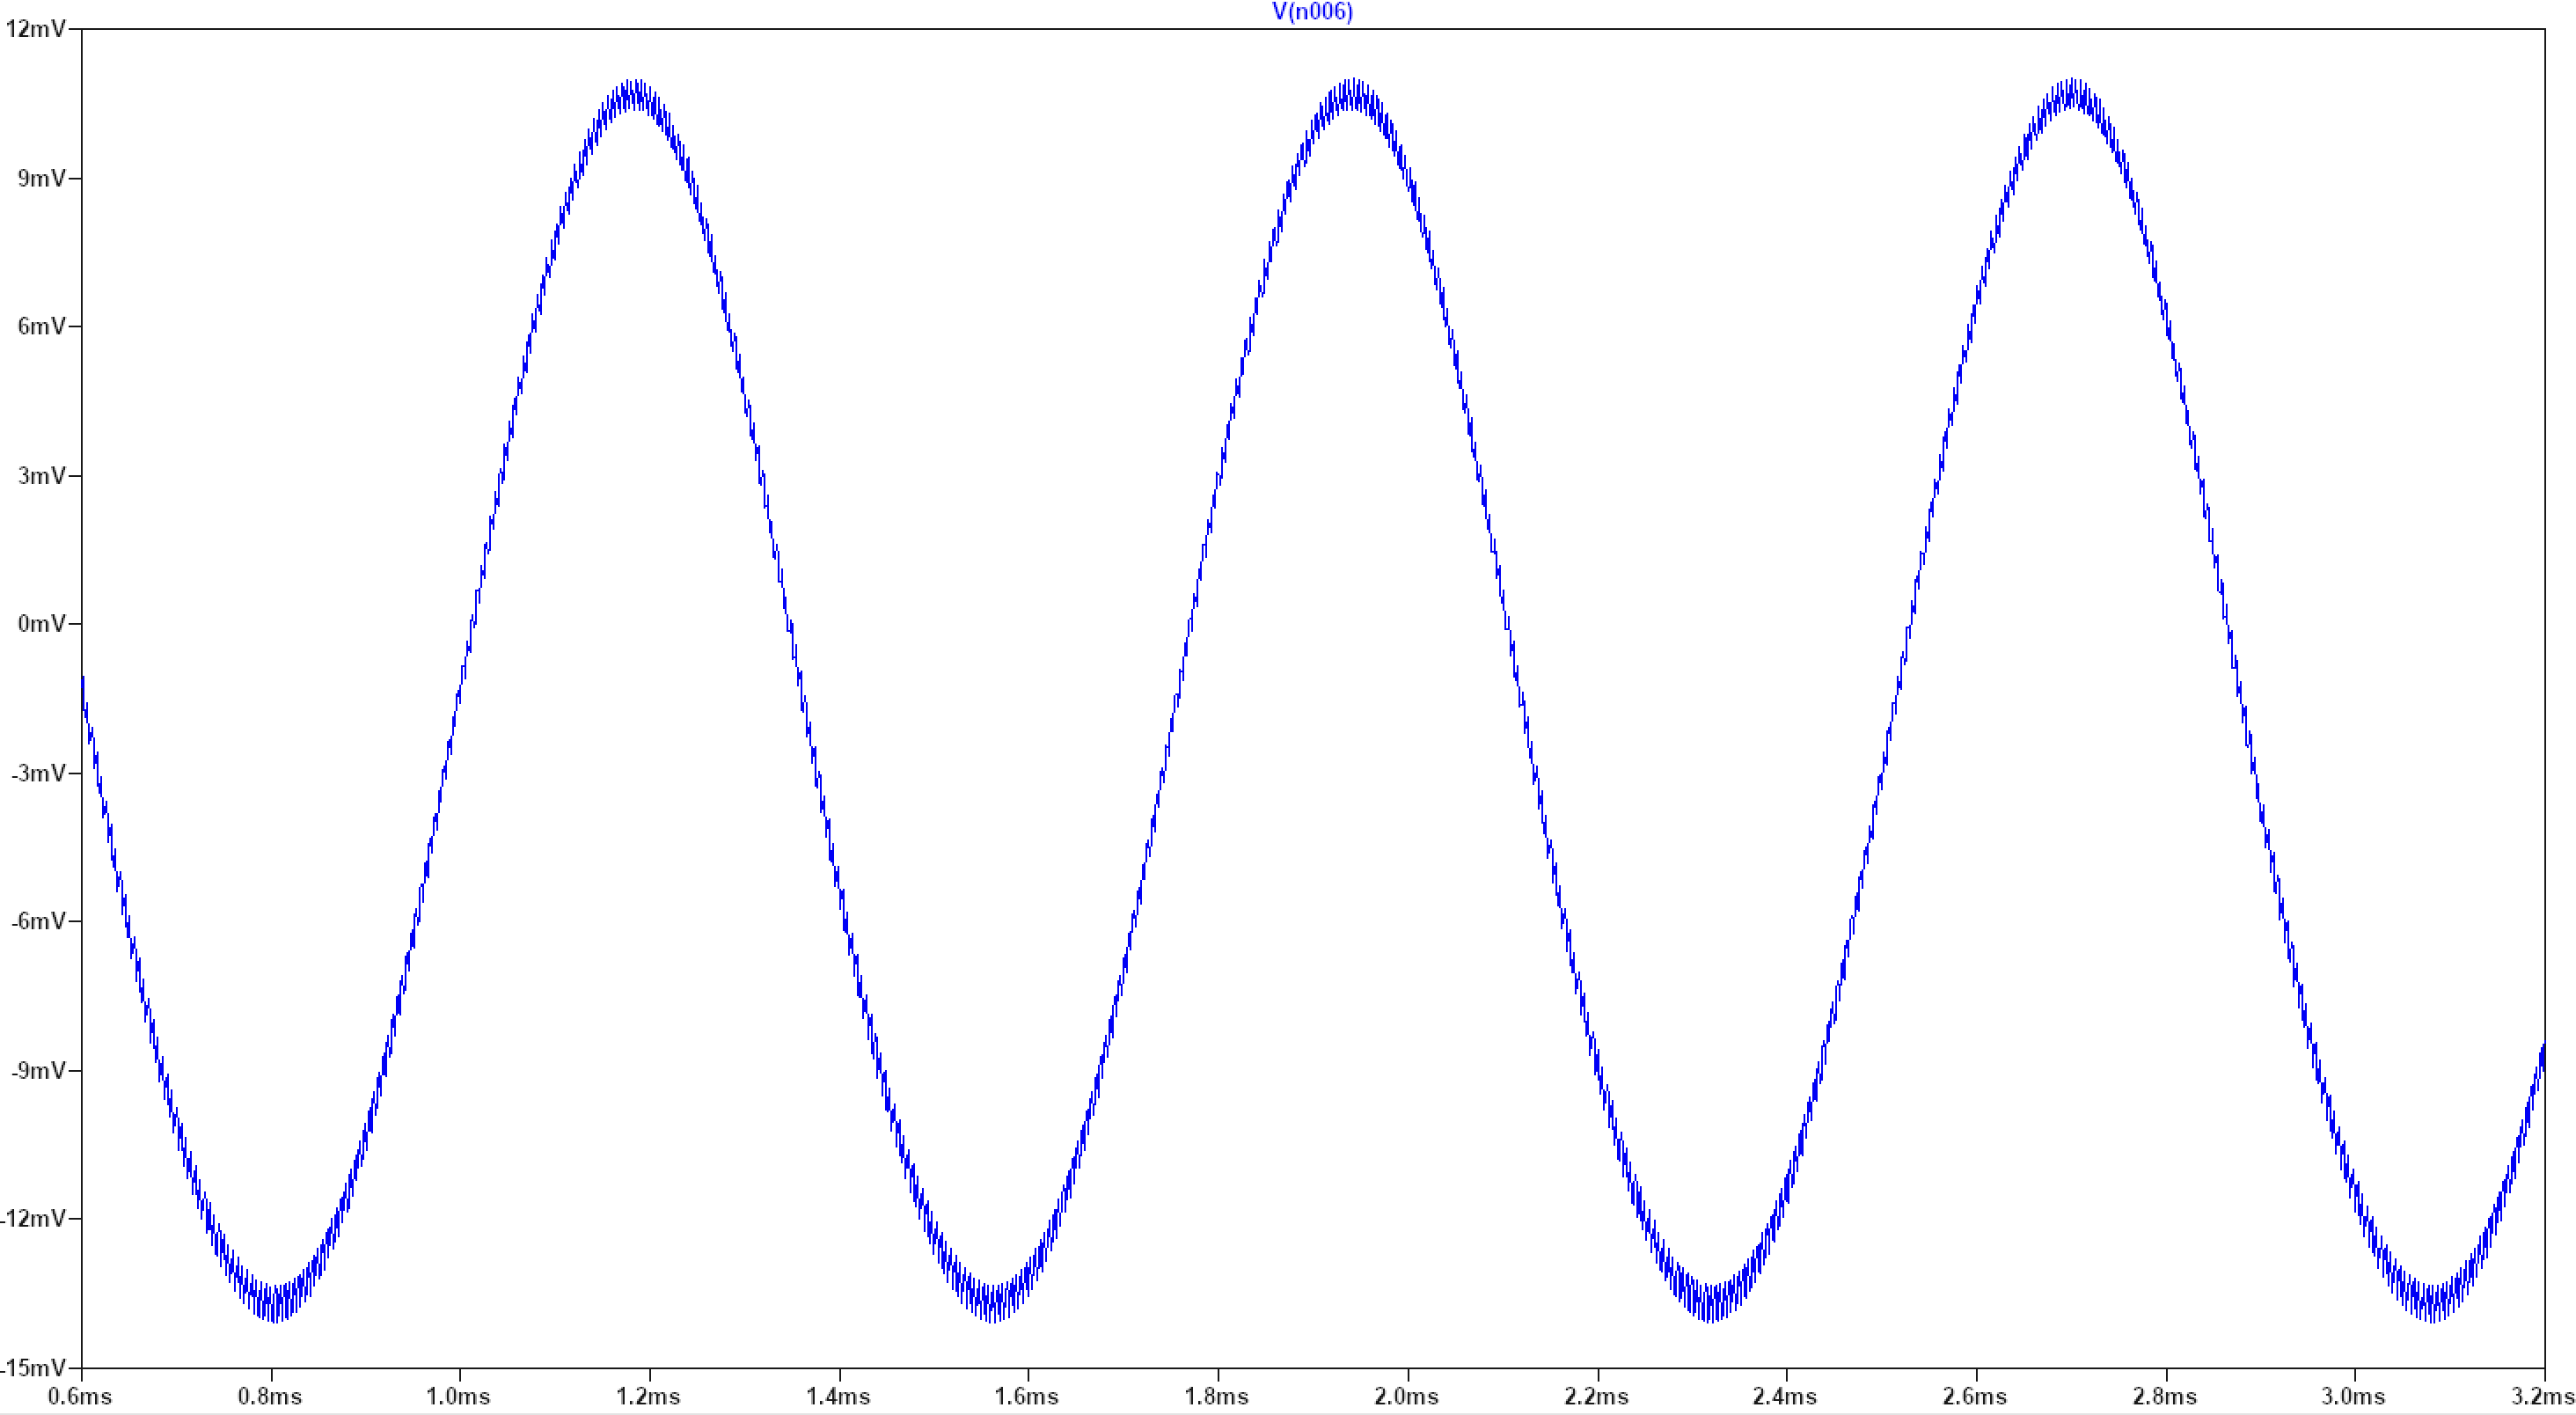
\includegraphics[width=0.9\linewidth]{../report/images/mixer+1lpf.png}
        \begin{itemize}
          \tiny
          \item Roll-off: $-20\text{ dB/decade}$.
          \item \textbf{Drawback:} High-frequency switching noise and $335\text{ kHz}$ sum harmonic bleed through.
        \end{itemize}
      \end{block}
    \end{column}
    \begin{column}{0.5\textwidth}
      \begin{block}{Iteration 2: Two-Stage Cascaded LPF}
        \centering
        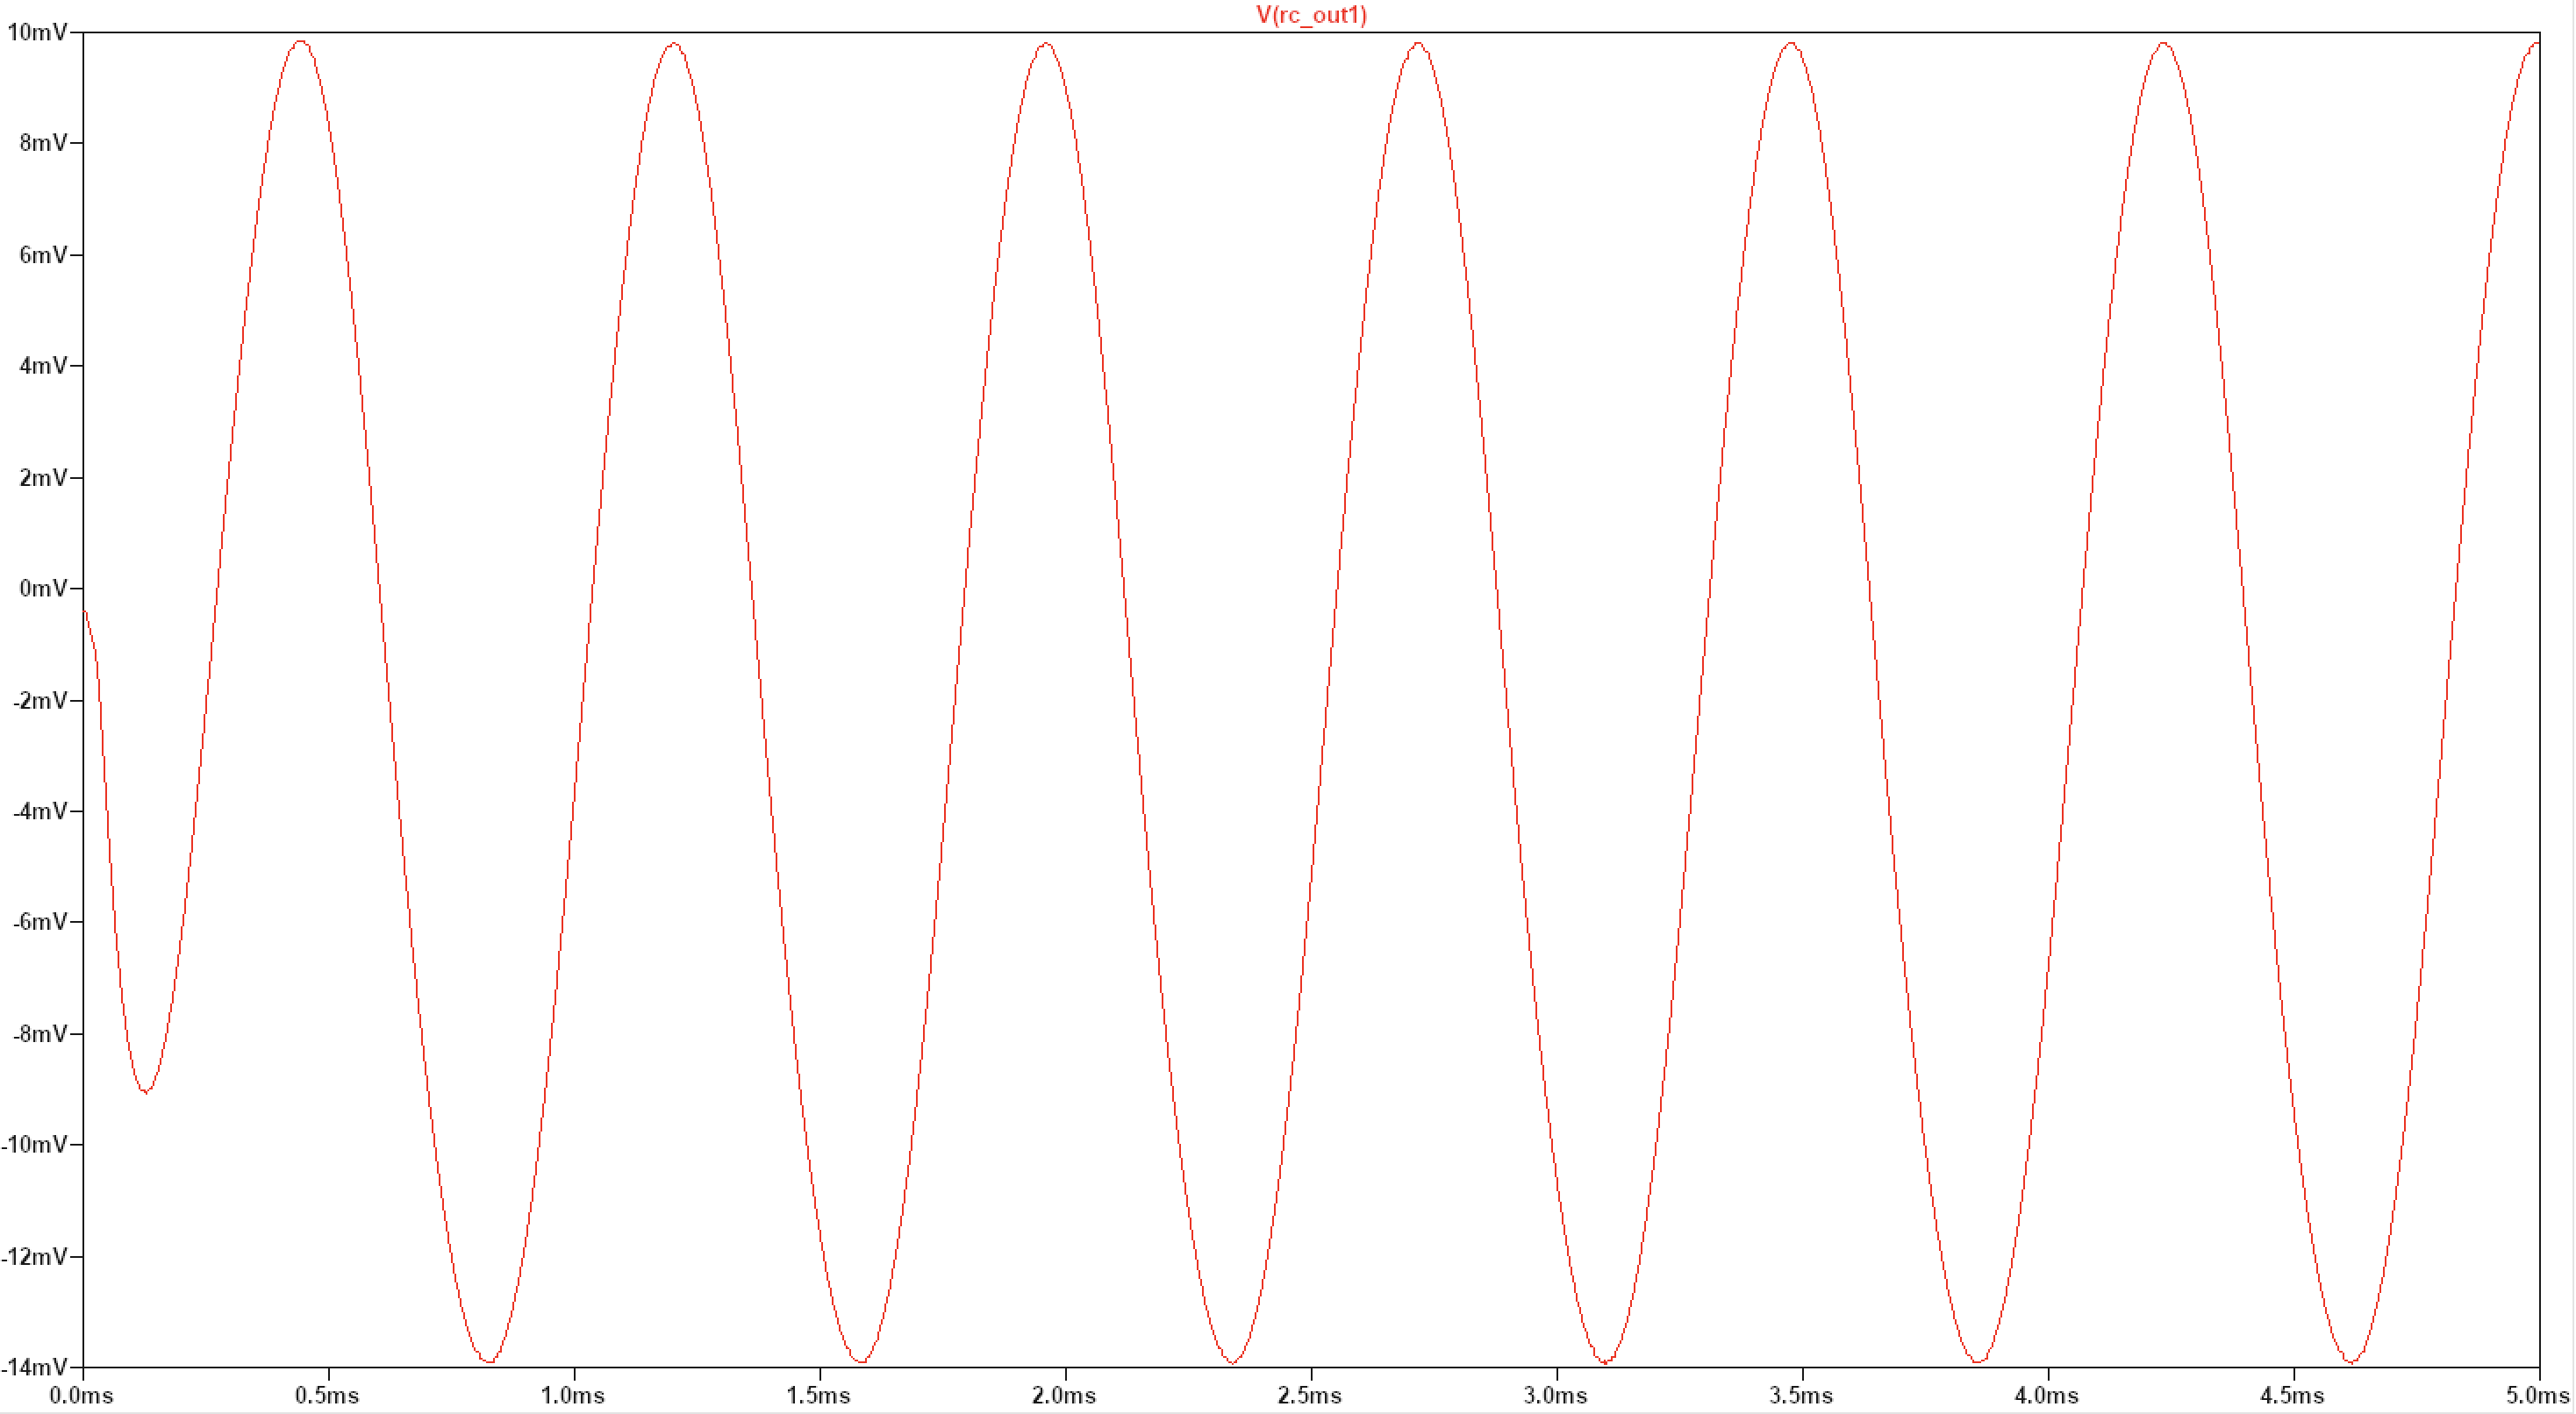
\includegraphics[width=0.9\linewidth]{../report/images/mixer+2lpf.png}
        \begin{itemize}
          \tiny
          \item Components: $2 \times (2.2\text{ k}\Omega, 10\text{ nF})$.
          \item Roll-off: $-40\text{ dB/decade}$.
          \item $f_{c,\text{cascaded}} \approx 7.23\text{ k} \times \sqrt{\sqrt{2}-1} \approx \mathbf{4.65\text{ kHz}}$.
        \end{itemize}
      \end{block}
    \end{column}
  \end{columns}
\end{frame}

% Slide 20: LPF Simulation & Hardware Bode Plot Verification
\begin{frame}{LPF Hardware Bode Plot \& Transient Response}
  \begin{columns}
    \begin{column}{0.33\textwidth}
      \centering
      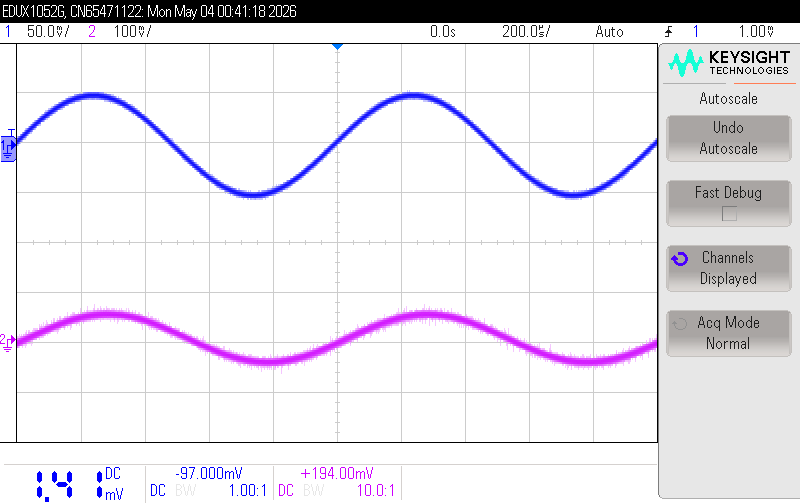
\includegraphics[width=0.92\linewidth]{../report/images/lpf1k.png} \\
      \vspace{0.02cm}
      \tiny $1\text{ kHz}$ Passband Response
    \end{column}
    \begin{column}{0.33\textwidth}
      \centering
      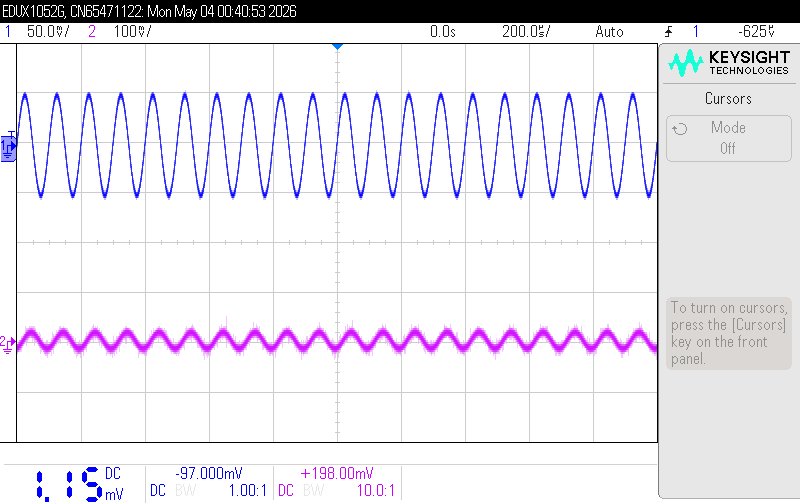
\includegraphics[width=0.92\linewidth]{../report/images/lpf10k.png} \\
      \vspace{0.02cm}
      \tiny $10\text{ kHz}$ Attenuated Response
    \end{column}
    \begin{column}{0.33\textwidth}
      \centering
      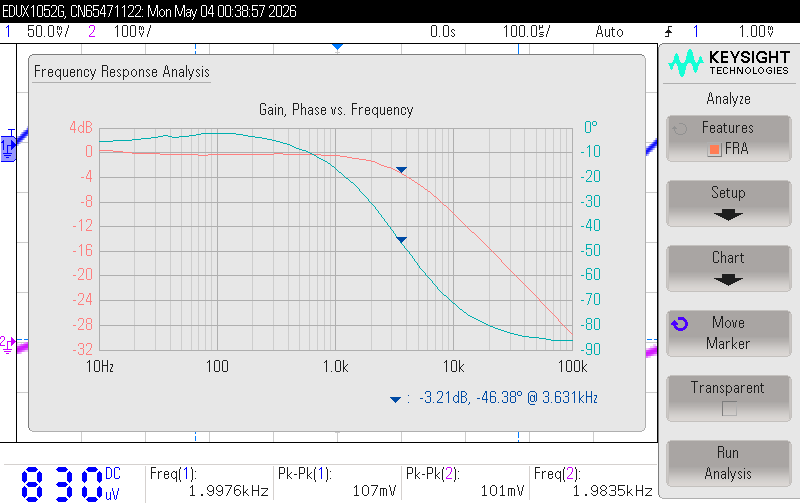
\includegraphics[width=0.92\linewidth]{../report/images/frequency-response-2.png} \\
      \vspace{0.02cm}
      \tiny Hardware Bode Plot (AC Response)
    \end{column}
  \end{columns}
  \vspace{0.05cm}
  \centering
  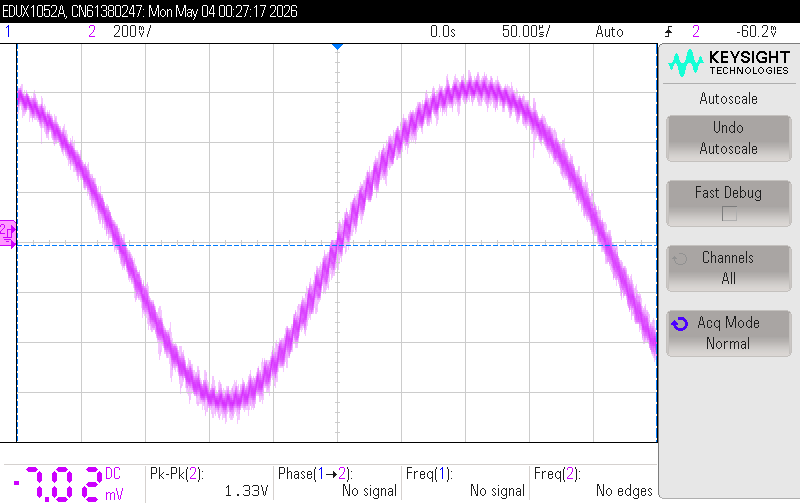
\includegraphics[width=0.52\linewidth]{../report/images/low-pass-output.png} \\
  \tiny DSO Capture: Integrated Mixer + Cascaded LPF Output ($5\text{ kHz}$ IF Tone).
\end{frame}

% Slide 21: CE BJT Amplifier Design (Discrete Stage)
\begin{frame}{CE BJT Amplifier Design (Discrete Gain Stage)}
  \begin{itemize}
    \item \textbf{Amplifier Topology Selection:} Implemented a discrete \textbf{Common Emitter (CE) BJT Amplifier} for output signal boosting.
    \item \textbf{Problem Statement:} Filter attenuation reduces $5\text{ kHz}$ IF to $\sim 8\text{ mV}$. Target specification requires $\ge 400\text{ mV}_{\text{pp}}$.
    \item \textbf{Emitter Degeneration ($R_{E1} = 15\,\Omega$) for Low THD:}
    \begin{align*}
      I_E &\approx 1.46\text{ mA} \implies r_e = \frac{V_T}{I_E} \approx \frac{26\text{ mV}}{1.46\text{ mA}} \approx 17.8\,\Omega \\
      A_v &\approx \frac{R_C}{R_{E1} + r_e} = \frac{2000}{15 + 17.8} \approx \mathbf{61} \\
      V_{\text{out}} &= V_{\text{in}} \times A_v \approx 8\text{ mV} \times 61 \approx \mathbf{488\text{ mV}_{\text{pp}}}
    \end{align*}
    \item \textbf{Result:} $488\text{ mV}_{\text{pp}}$ swing comfortably satisfies the $\ge 400\text{ mV}_{\text{pp}}$ specification.
  \end{itemize}
\end{frame}

% Slide 22: Amplifier Hardware Implementation & Integrated Response
\begin{frame}{Amplifier Lab Setup \& Output Swing}
  \begin{columns}
    \begin{column}{0.5\textwidth}
      \centering
      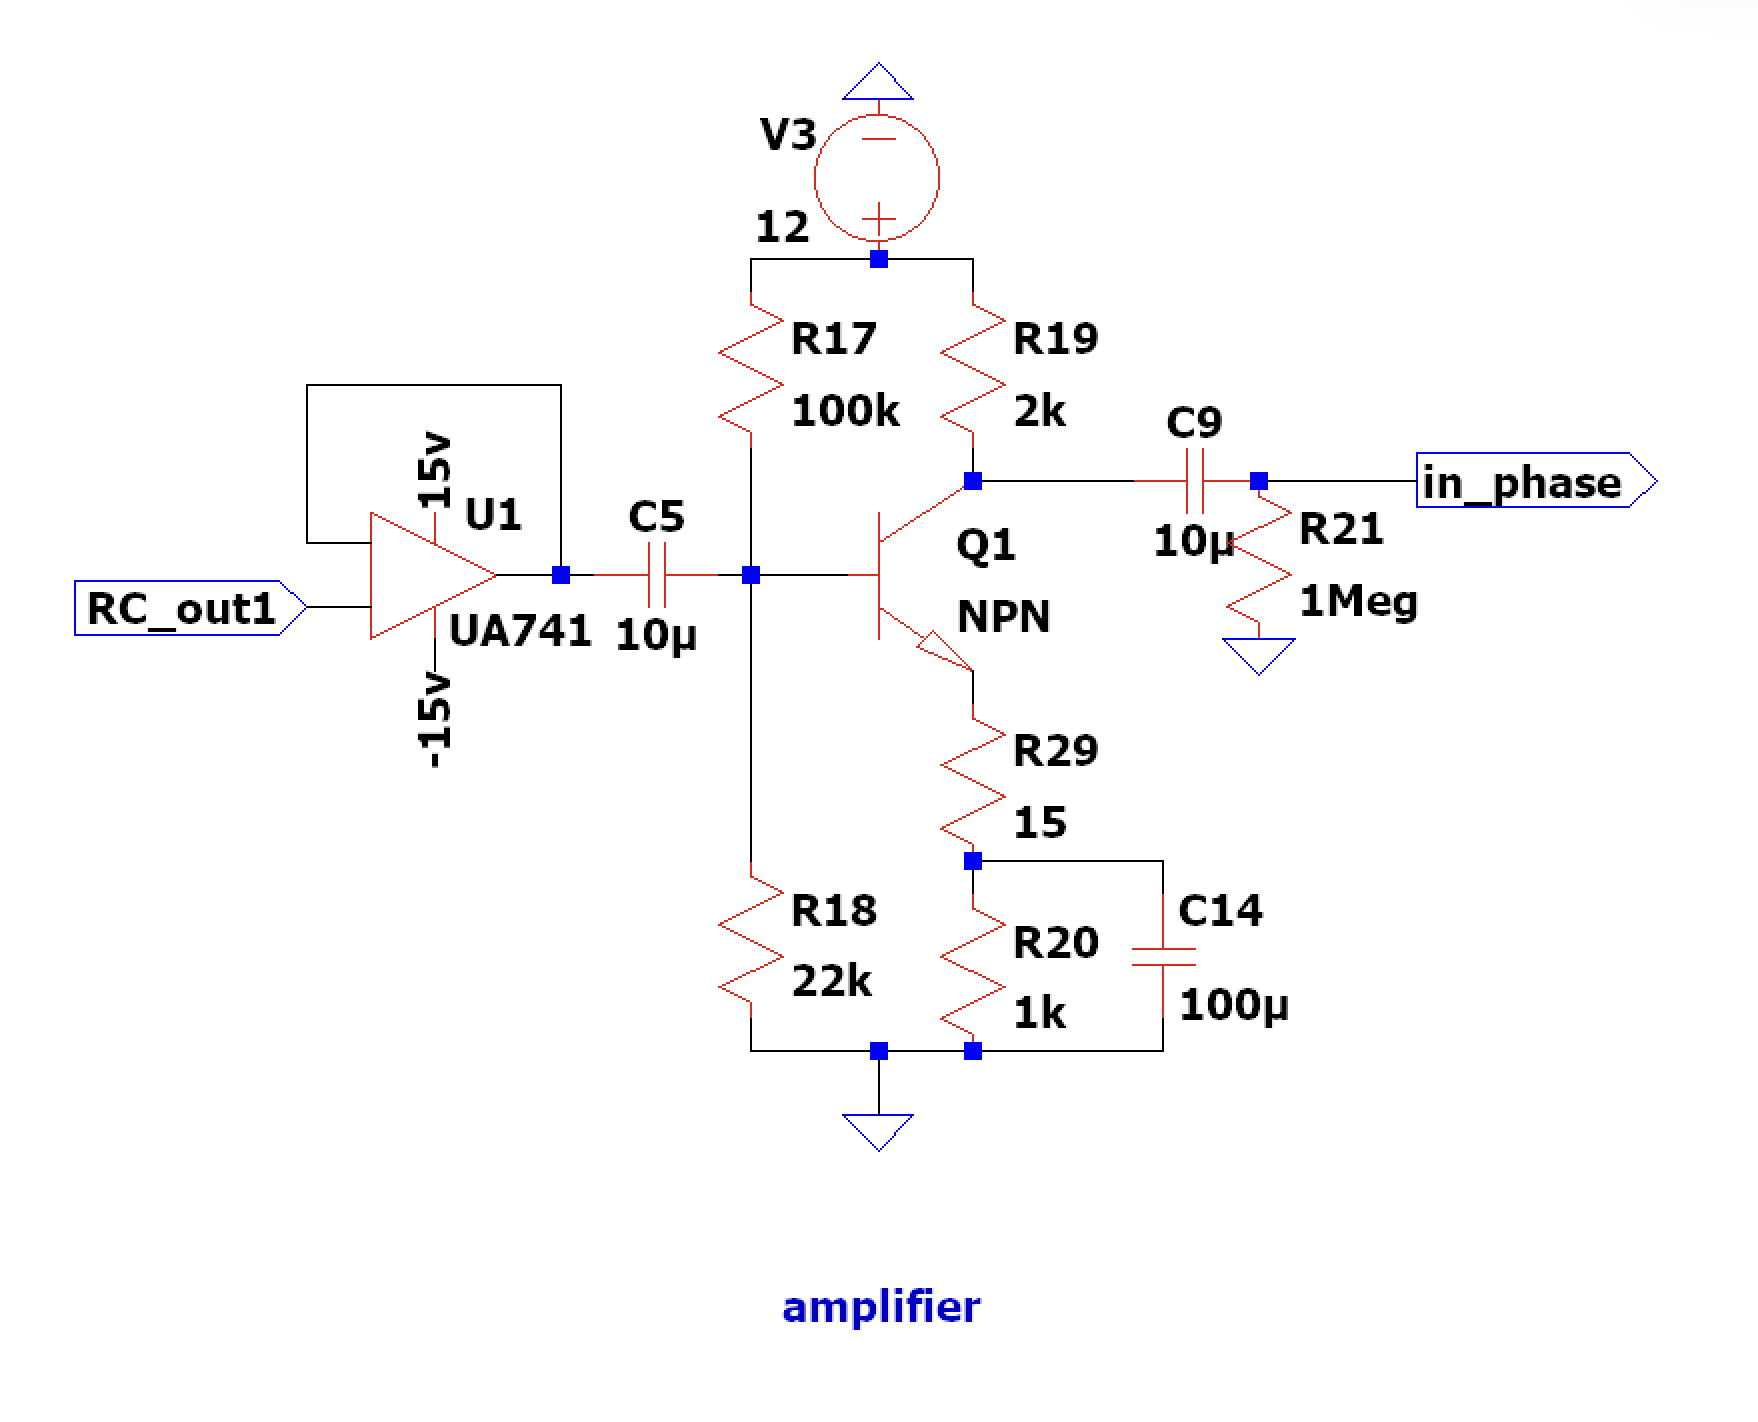
\includegraphics[width=0.88\linewidth]{../report/images/amplifier.png}
      \vspace{0.1cm}
      \tiny (a) Hardware Breadboard Setup of CE BJT Amplifier.
    \end{column}
    \begin{column}{0.5\textwidth}
      \centering
      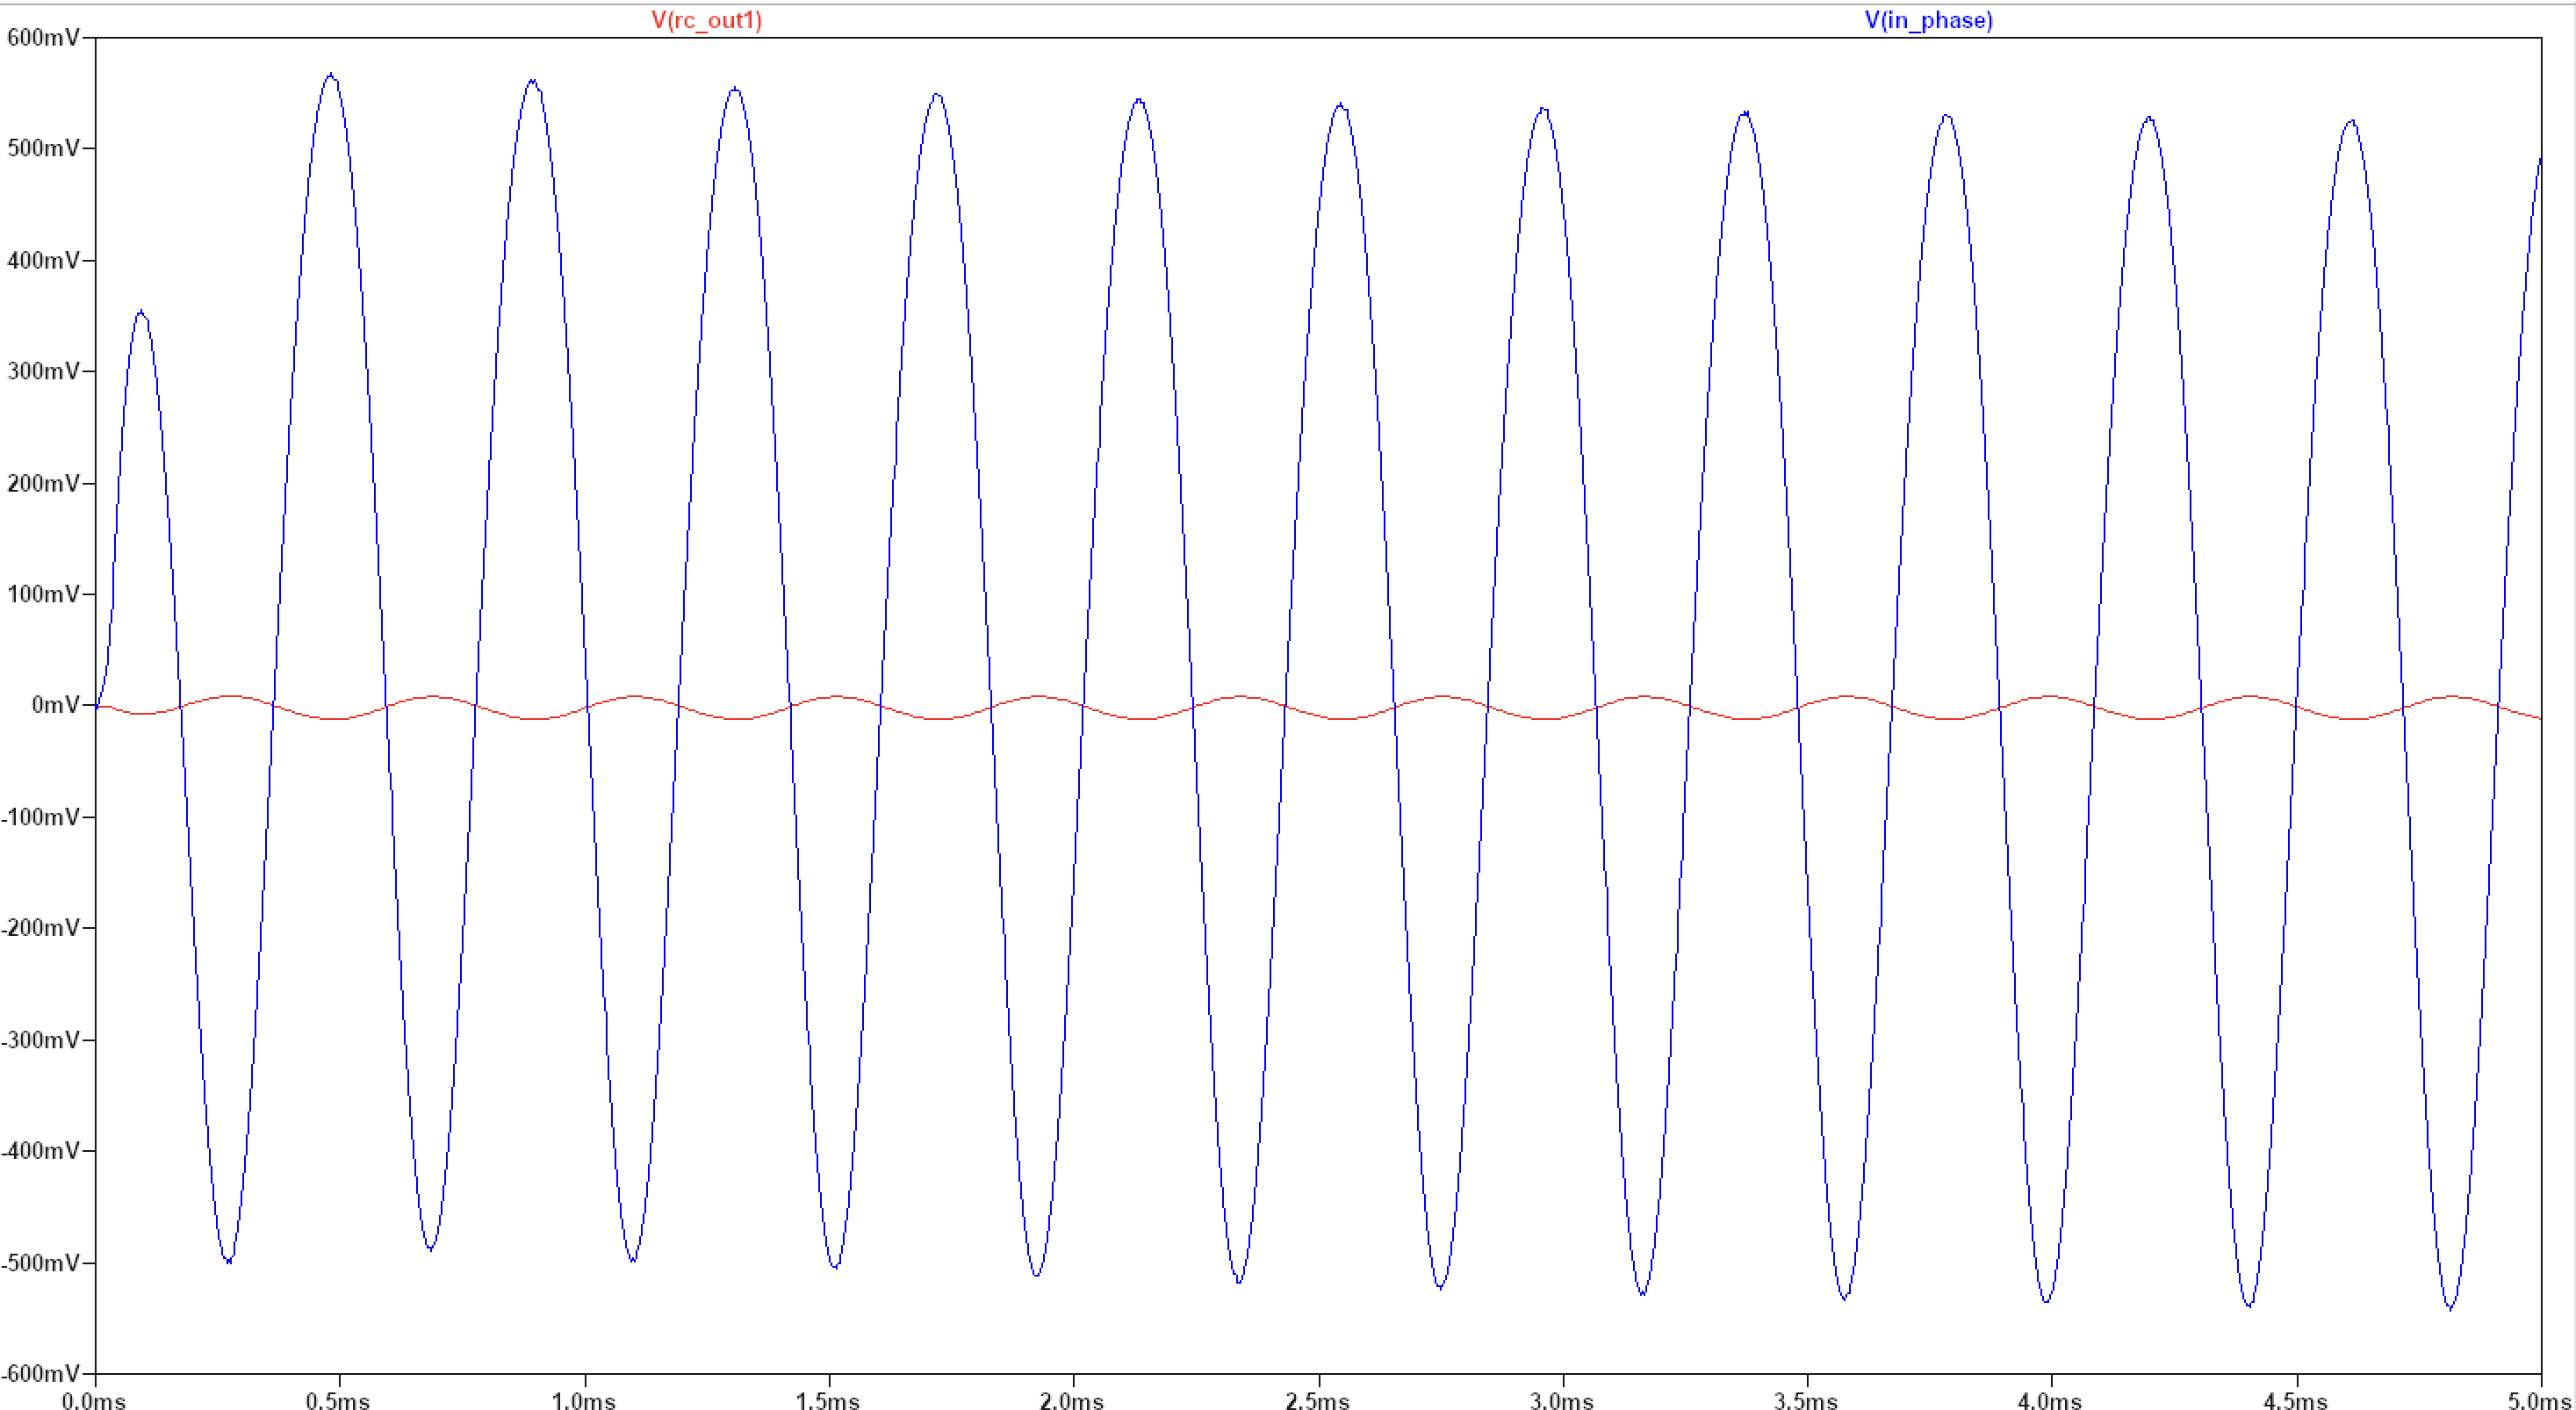
\includegraphics[width=\linewidth]{../report/images/LPF+amp.png}
      \vspace{0.1cm}
      \tiny (b) Integrated DSO Output: Mixer + LPF + Amplifier ($5\text{ kHz}$, $>450\text{ mV}_{\text{pp}}$).
    \end{column}
  \end{columns}
\end{frame}

\section{Complete Circuit Prototype \& Verification}

% Slide 23: Complete Prototype Schematic & Architecture
\begin{frame}{Complete Integrated QDC Prototype Schematic}
  \centering
  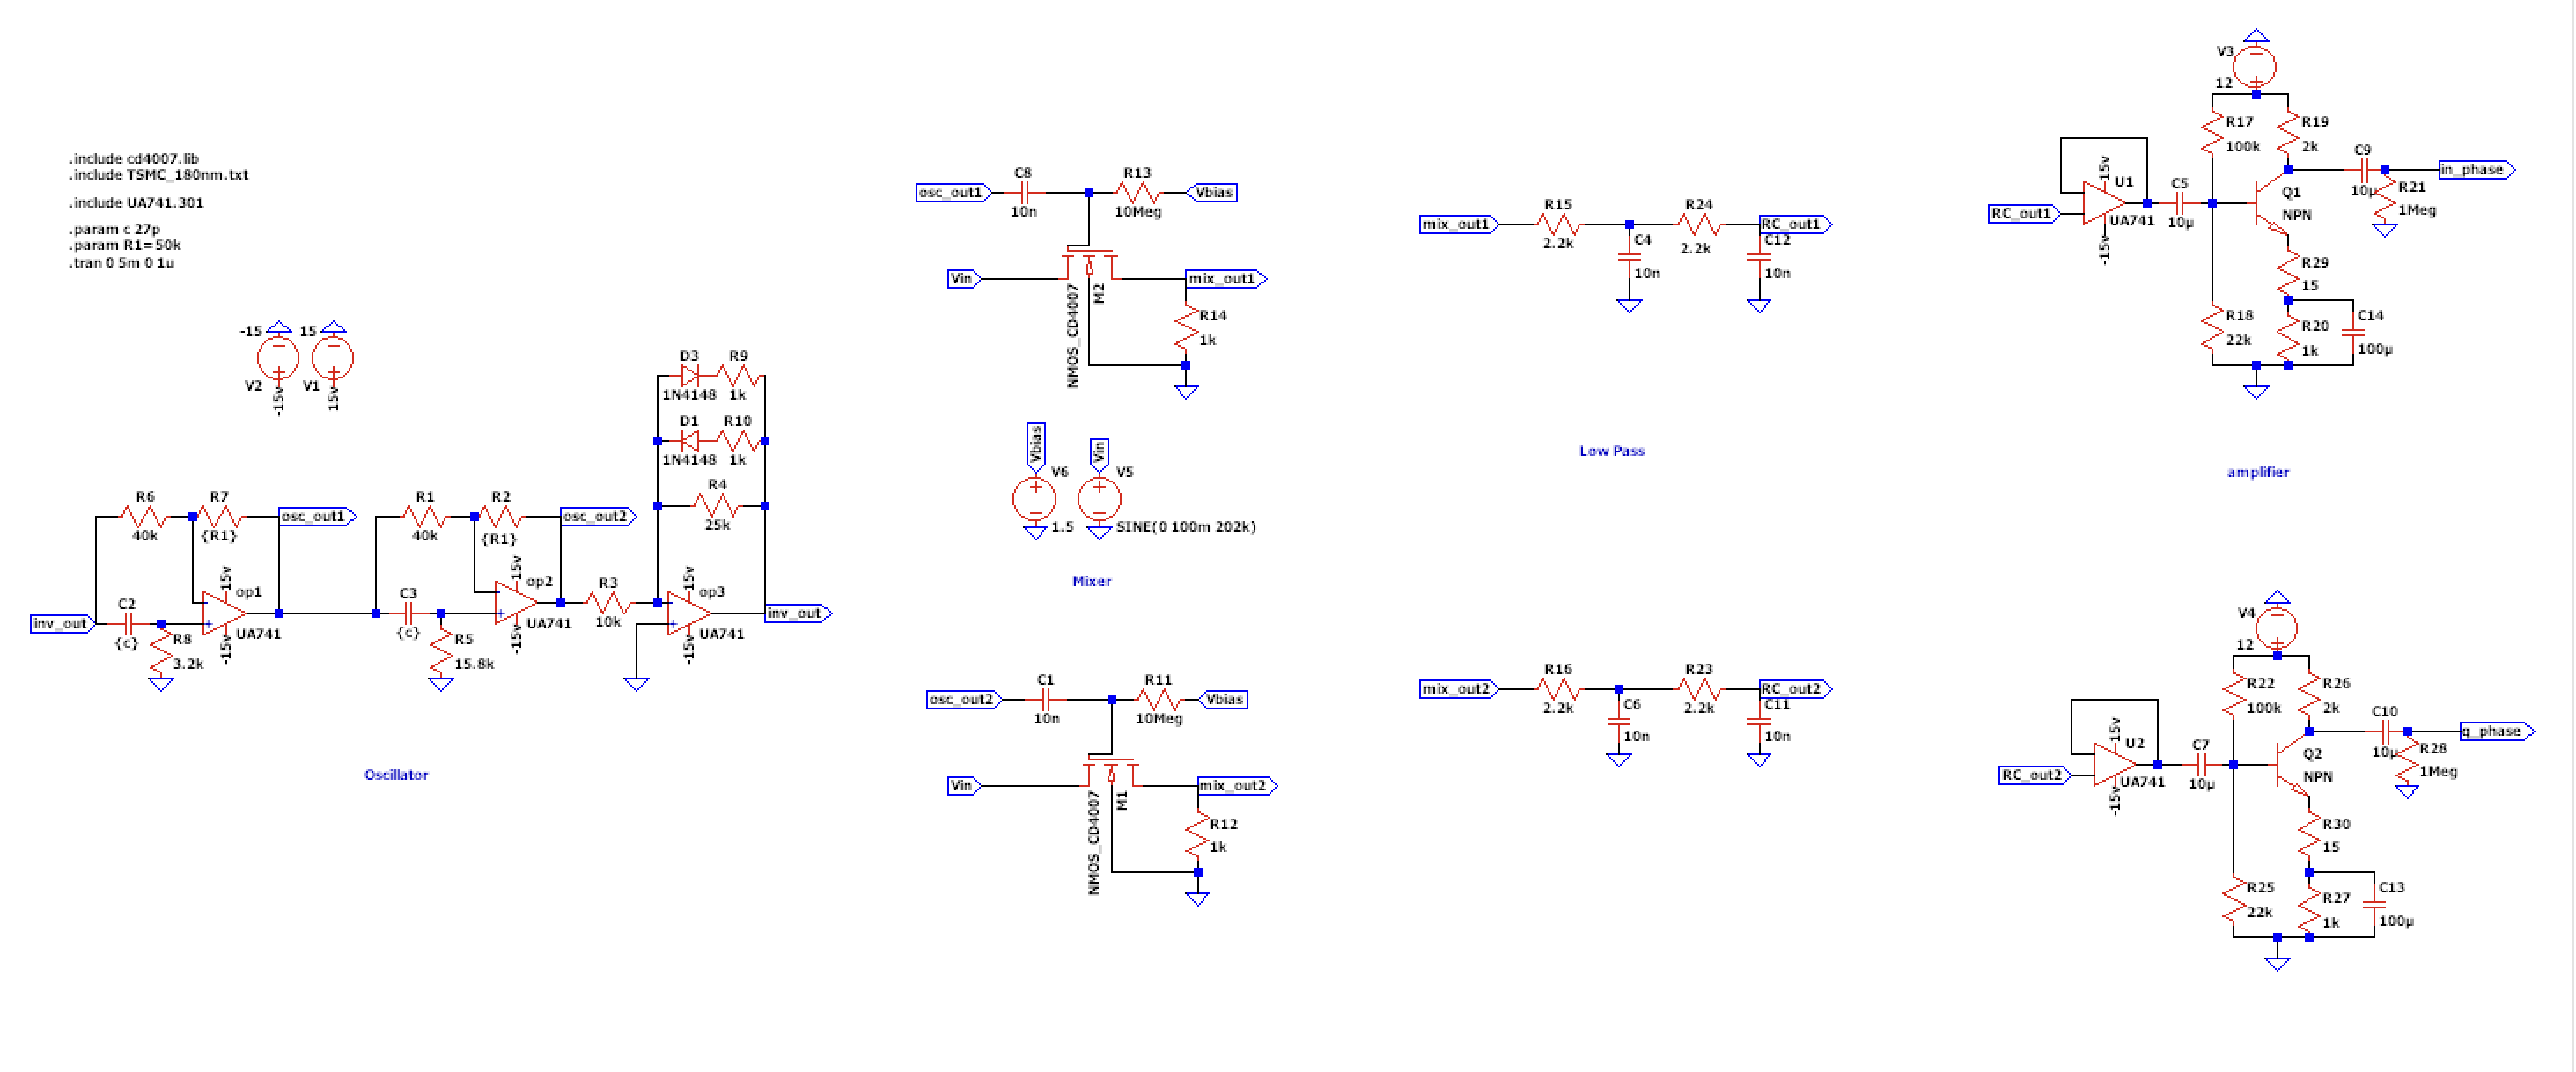
\includegraphics[width=0.88\linewidth]{../report/images/5-final_circ.png}
  \vspace{0.15cm}
  \begin{itemize}
    \scriptsize
    \item Complete QDC architecture integrating Quadrature Oscillator, dual NMOS Mixers, dual Cascaded LPFs, and dual CE BJT Amplifiers.
  \end{itemize}
\end{frame}

% Slide 24: Integrated System Simulation Results
\begin{frame}{System LTSpice Simulation Results}
  \begin{columns}
    \begin{column}{0.5\textwidth}
      \centering
      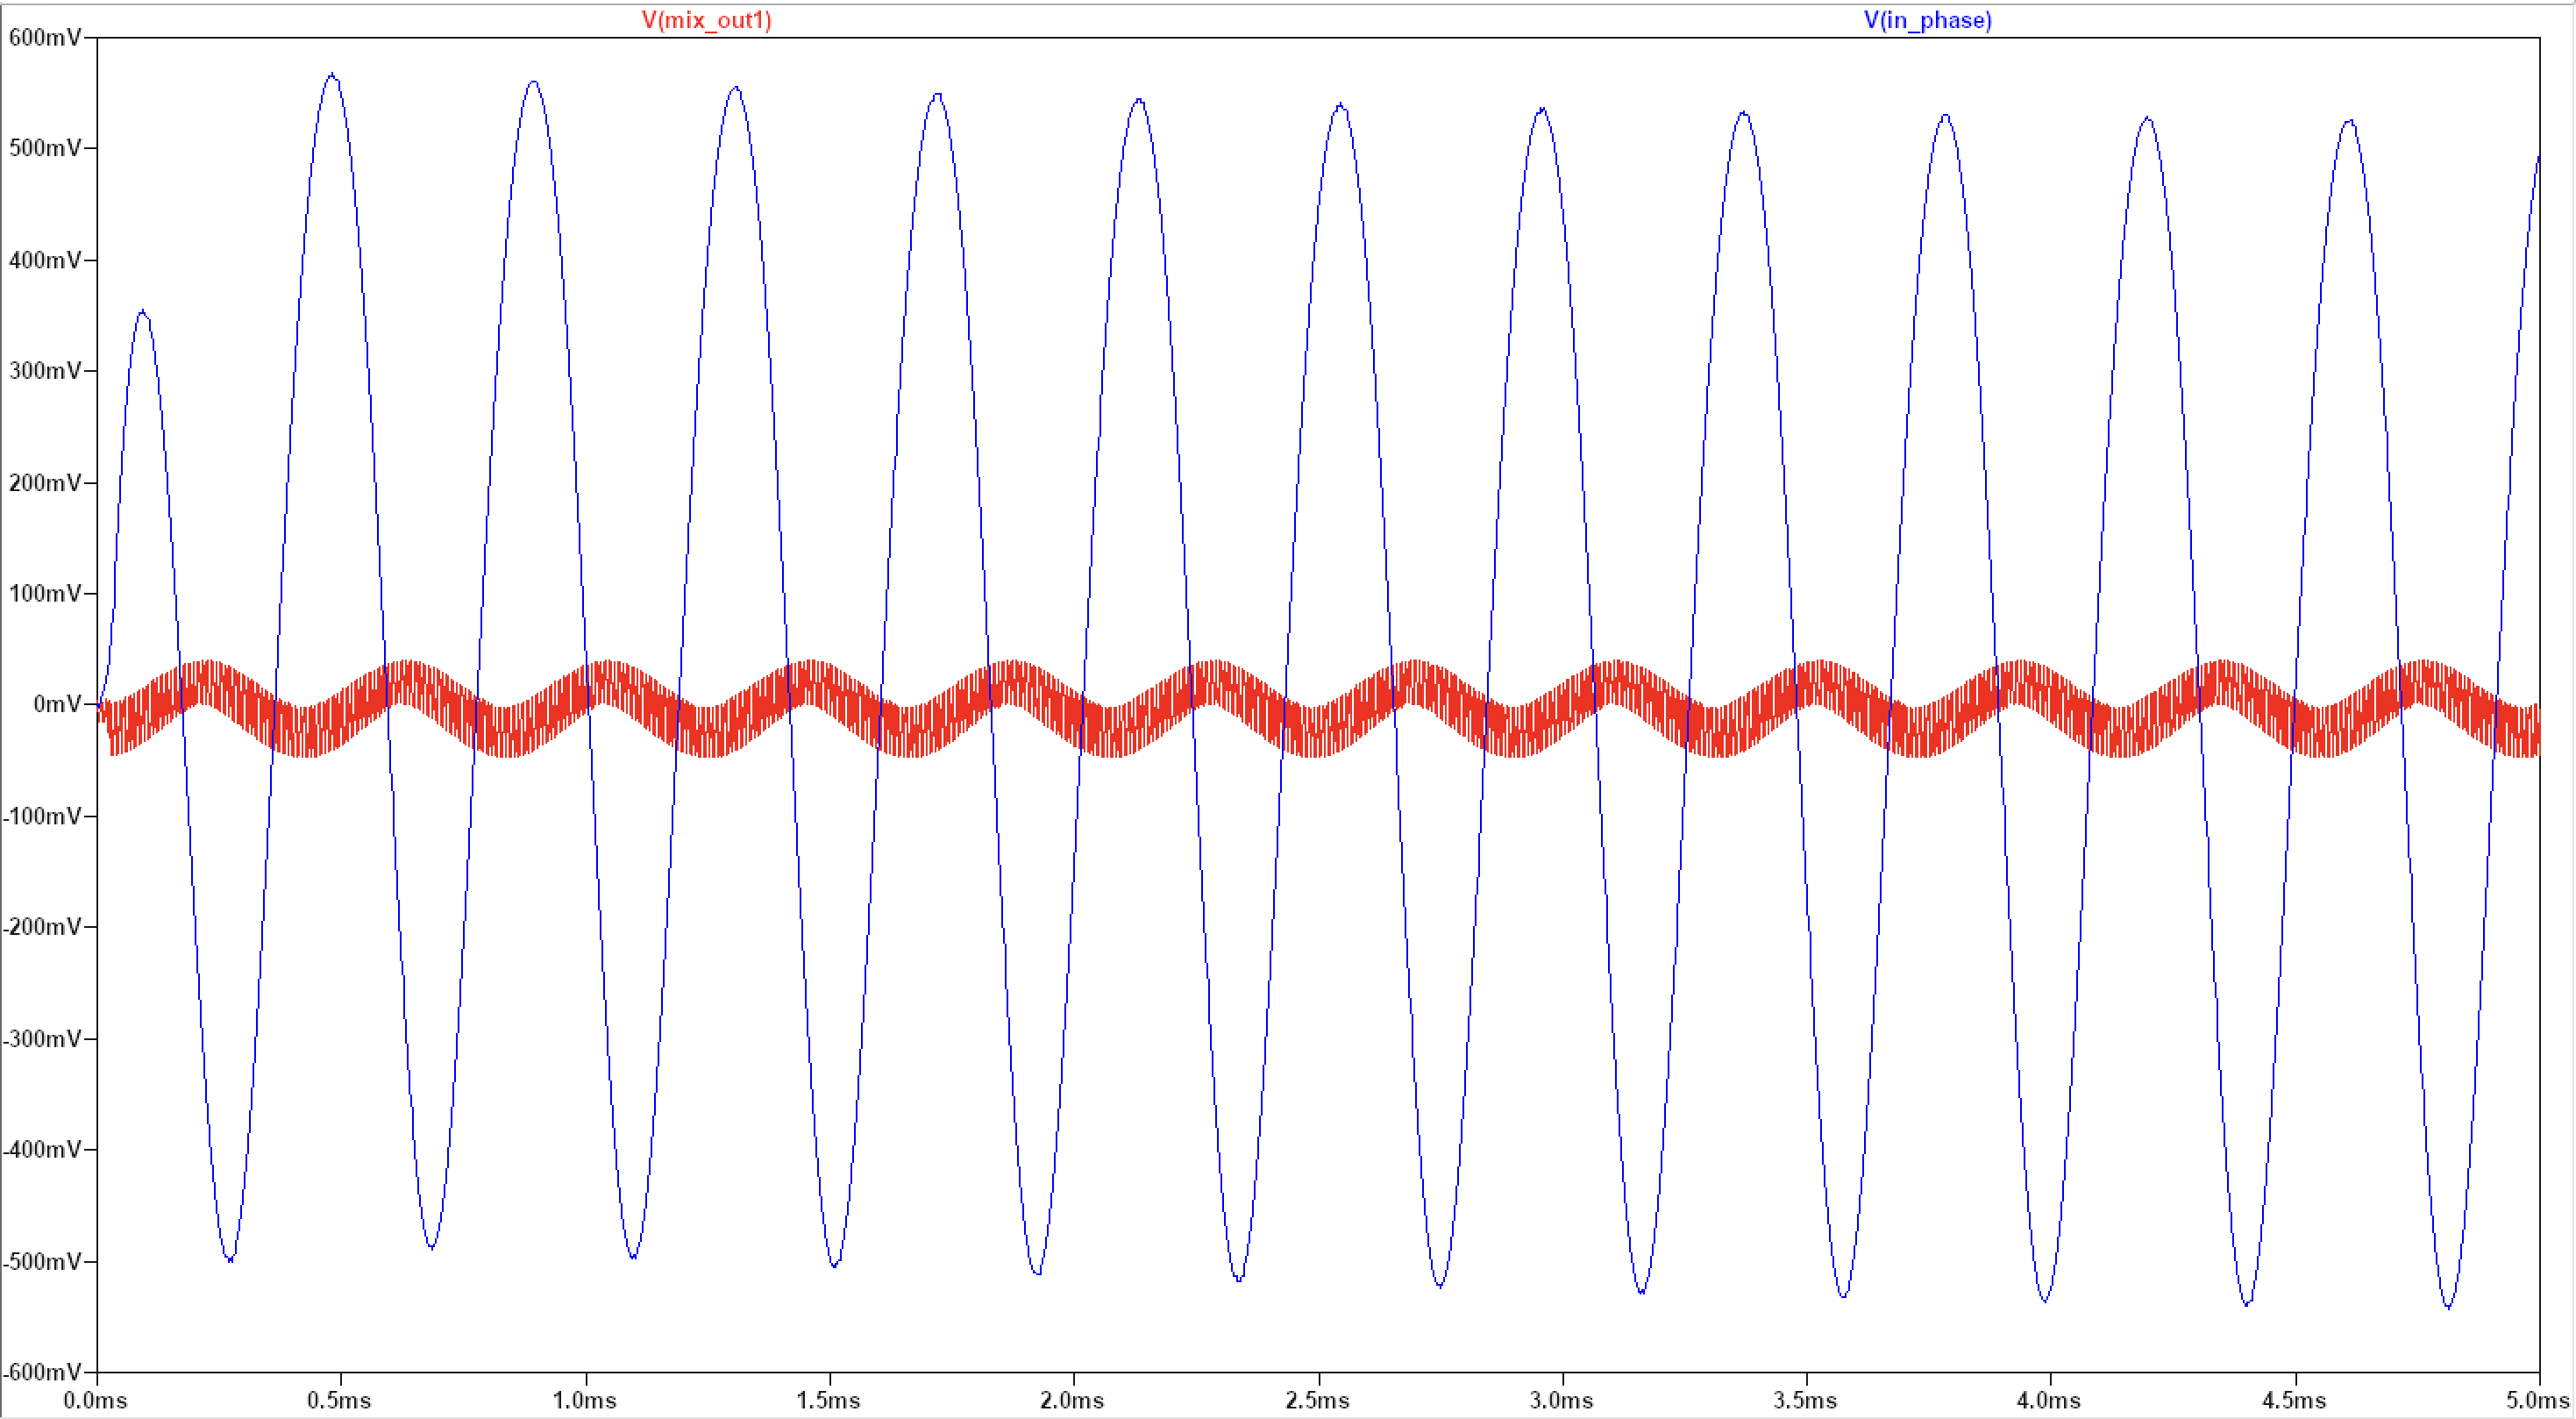
\includegraphics[width=\linewidth]{../report/images/5-If-If-final.png}
      \vspace{0.1cm}
      \tiny (a) Transient Simulation of Final $v_{IF\_FINAL\_I}$ and $v_{IF\_FINAL\_Q}$ Signals ($5\text{ kHz}, 90^\circ$).
    \end{column}
    \begin{column}{0.5\textwidth}
      \centering
      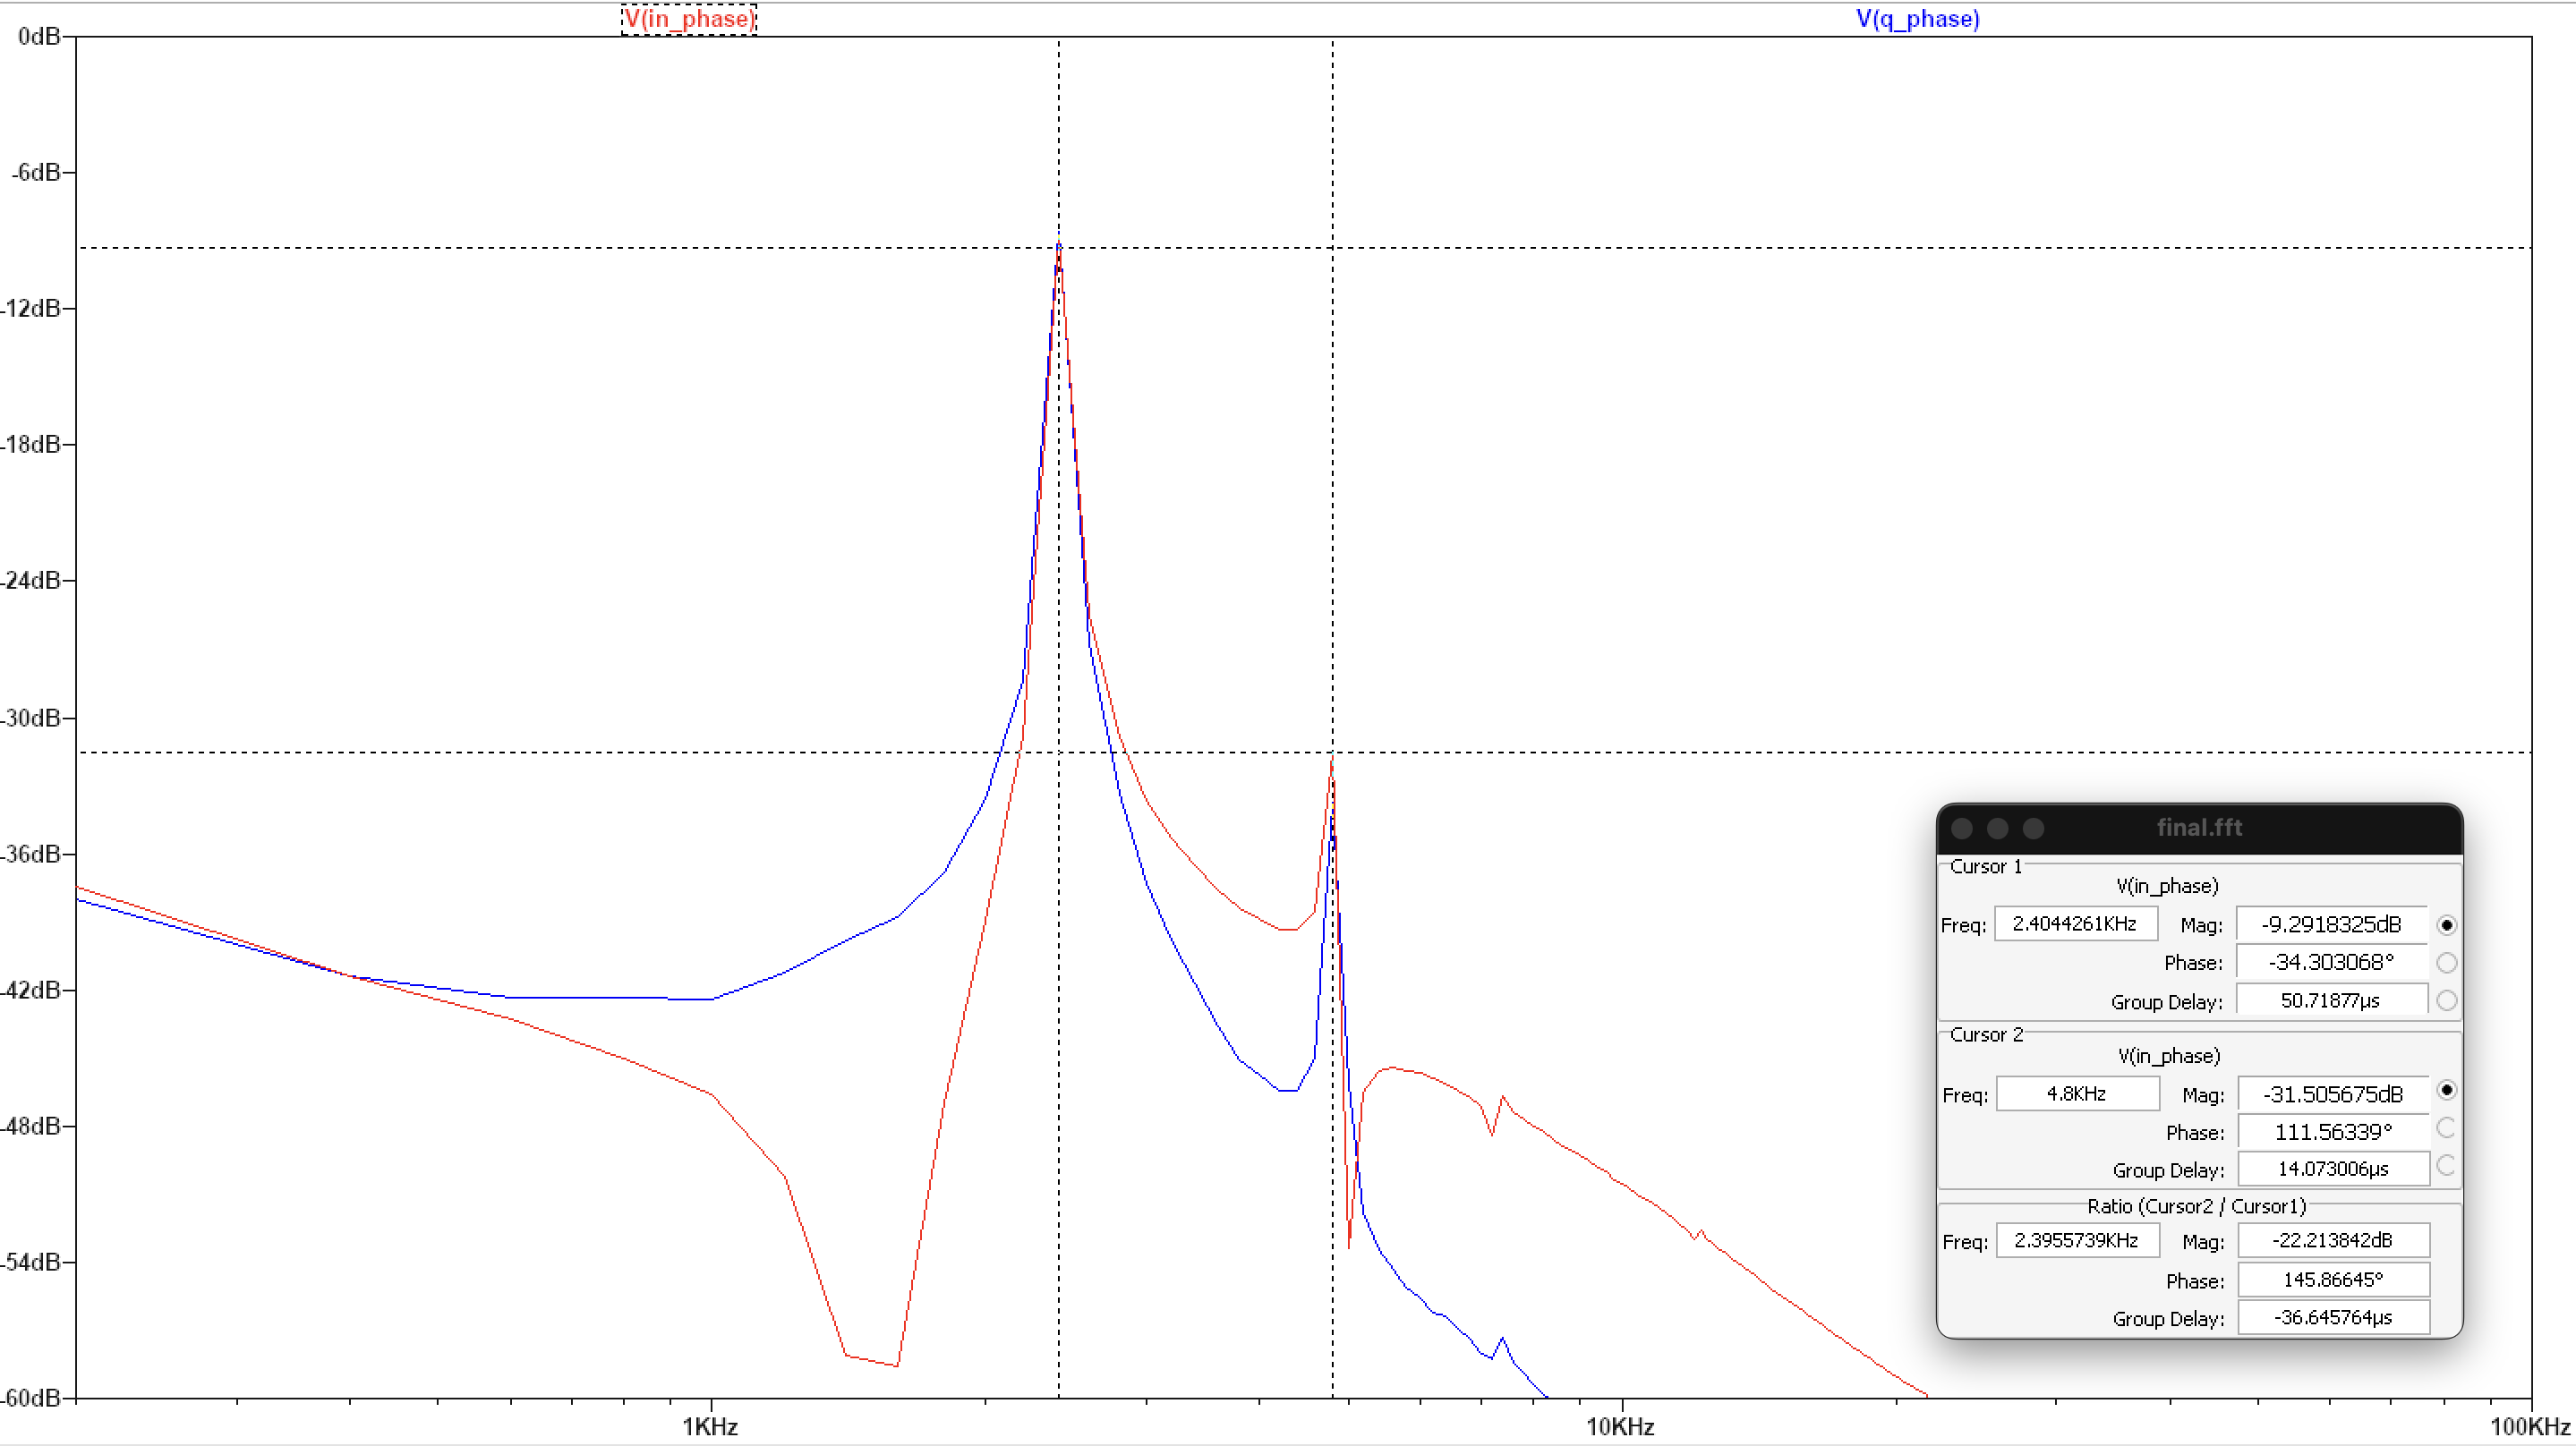
\includegraphics[width=\linewidth]{../report/images/5-iq-fft.png}
      \vspace{0.1cm}
      \tiny (b) FFT Spectrum of Final I and Q Outputs showing pure $5\text{ kHz}$ peaks.
    \end{column}
  \end{columns}
\end{frame}

% Slide 25: Hardware Verification - DSO Single & Envelope Captures
\begin{frame}{Hardware DSO Measurements -- Single \& Envelope}
  \begin{columns}
    \begin{column}{0.5\textwidth}
      \centering
      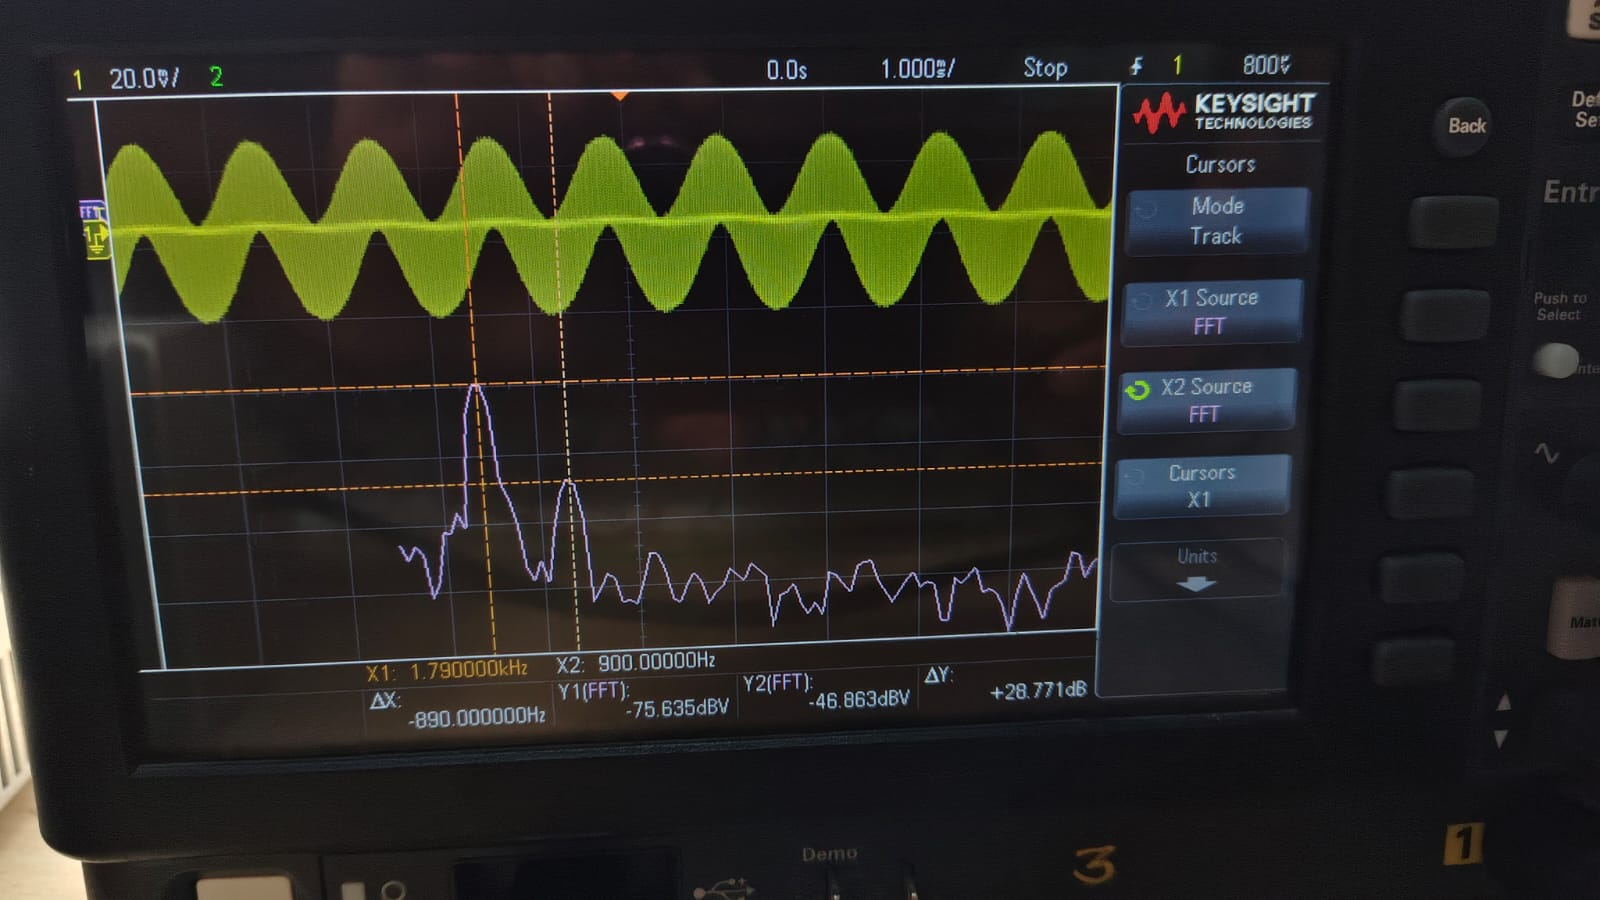
\includegraphics[width=\linewidth]{../report/images/5-Vif.jpeg}
      \vspace{0.1cm}
      \tiny (a) DSO Measurement: Single IF Channel Output ($5\text{ kHz}$).
    \end{column}
    \begin{column}{0.5\textwidth}
      \centering
      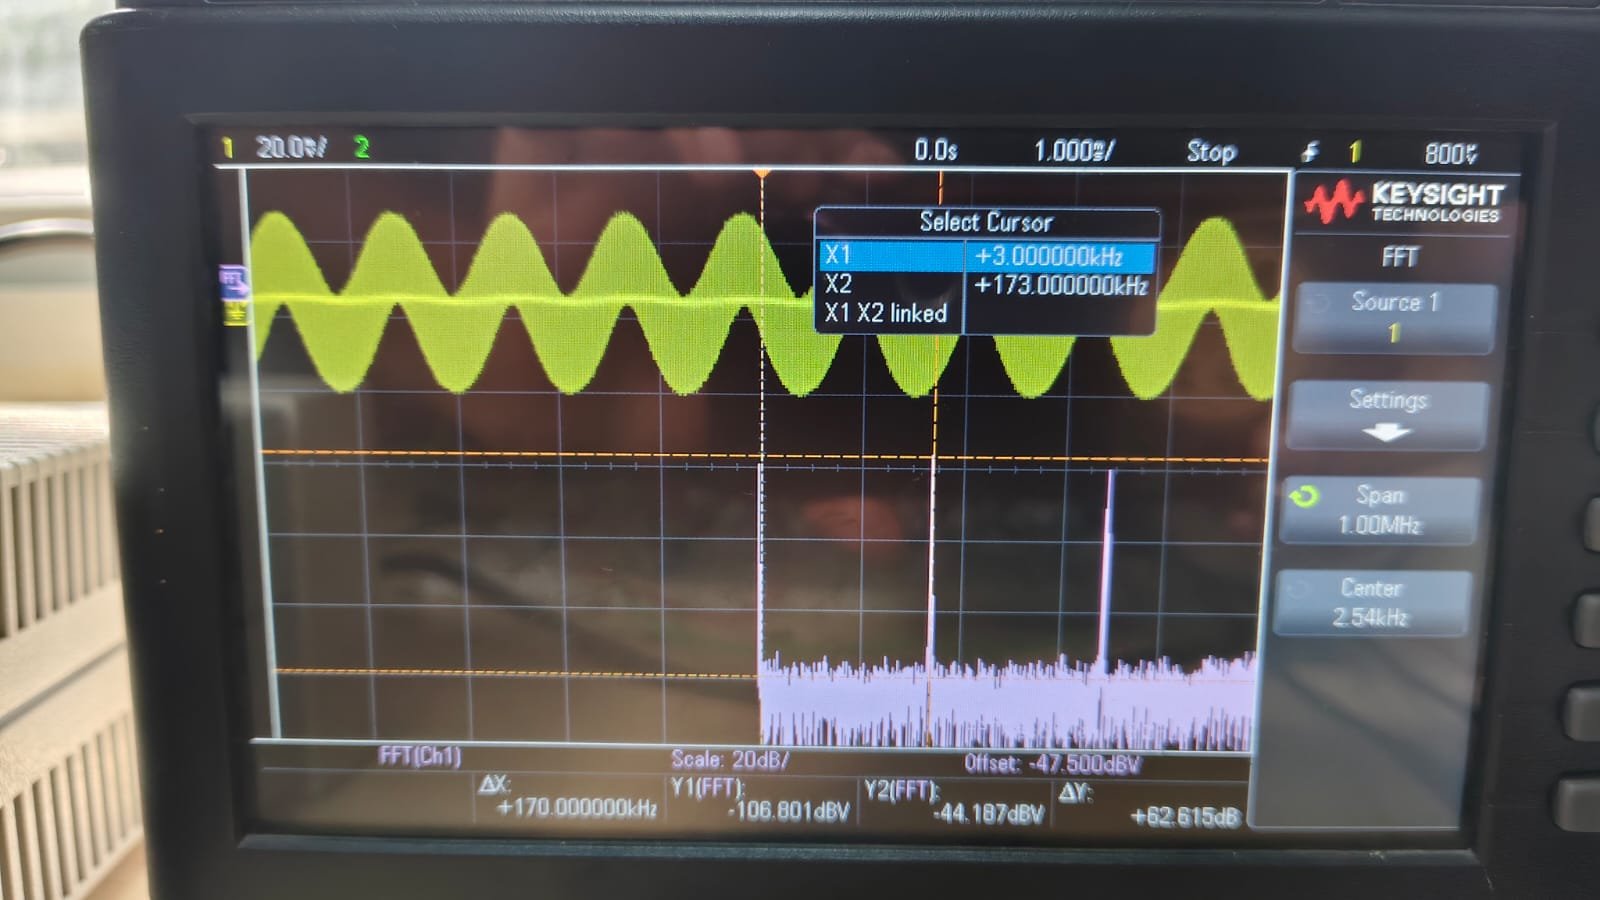
\includegraphics[width=\linewidth]{../report/images/5-vif+170.jpeg}
      \vspace{0.1cm}
      \tiny (b) DSO Measurement: IF Output overlaid with $170\text{ kHz}$ RF Input Envelope.
    \end{column}
  \end{columns}
\end{frame}

% Slide 26: Hardware Quadrature Phase Shift Verification
\begin{frame}{Hardware Quadrature Phase Shift Verification}
  \begin{columns}
    \begin{column}{0.5\textwidth}
      \centering
      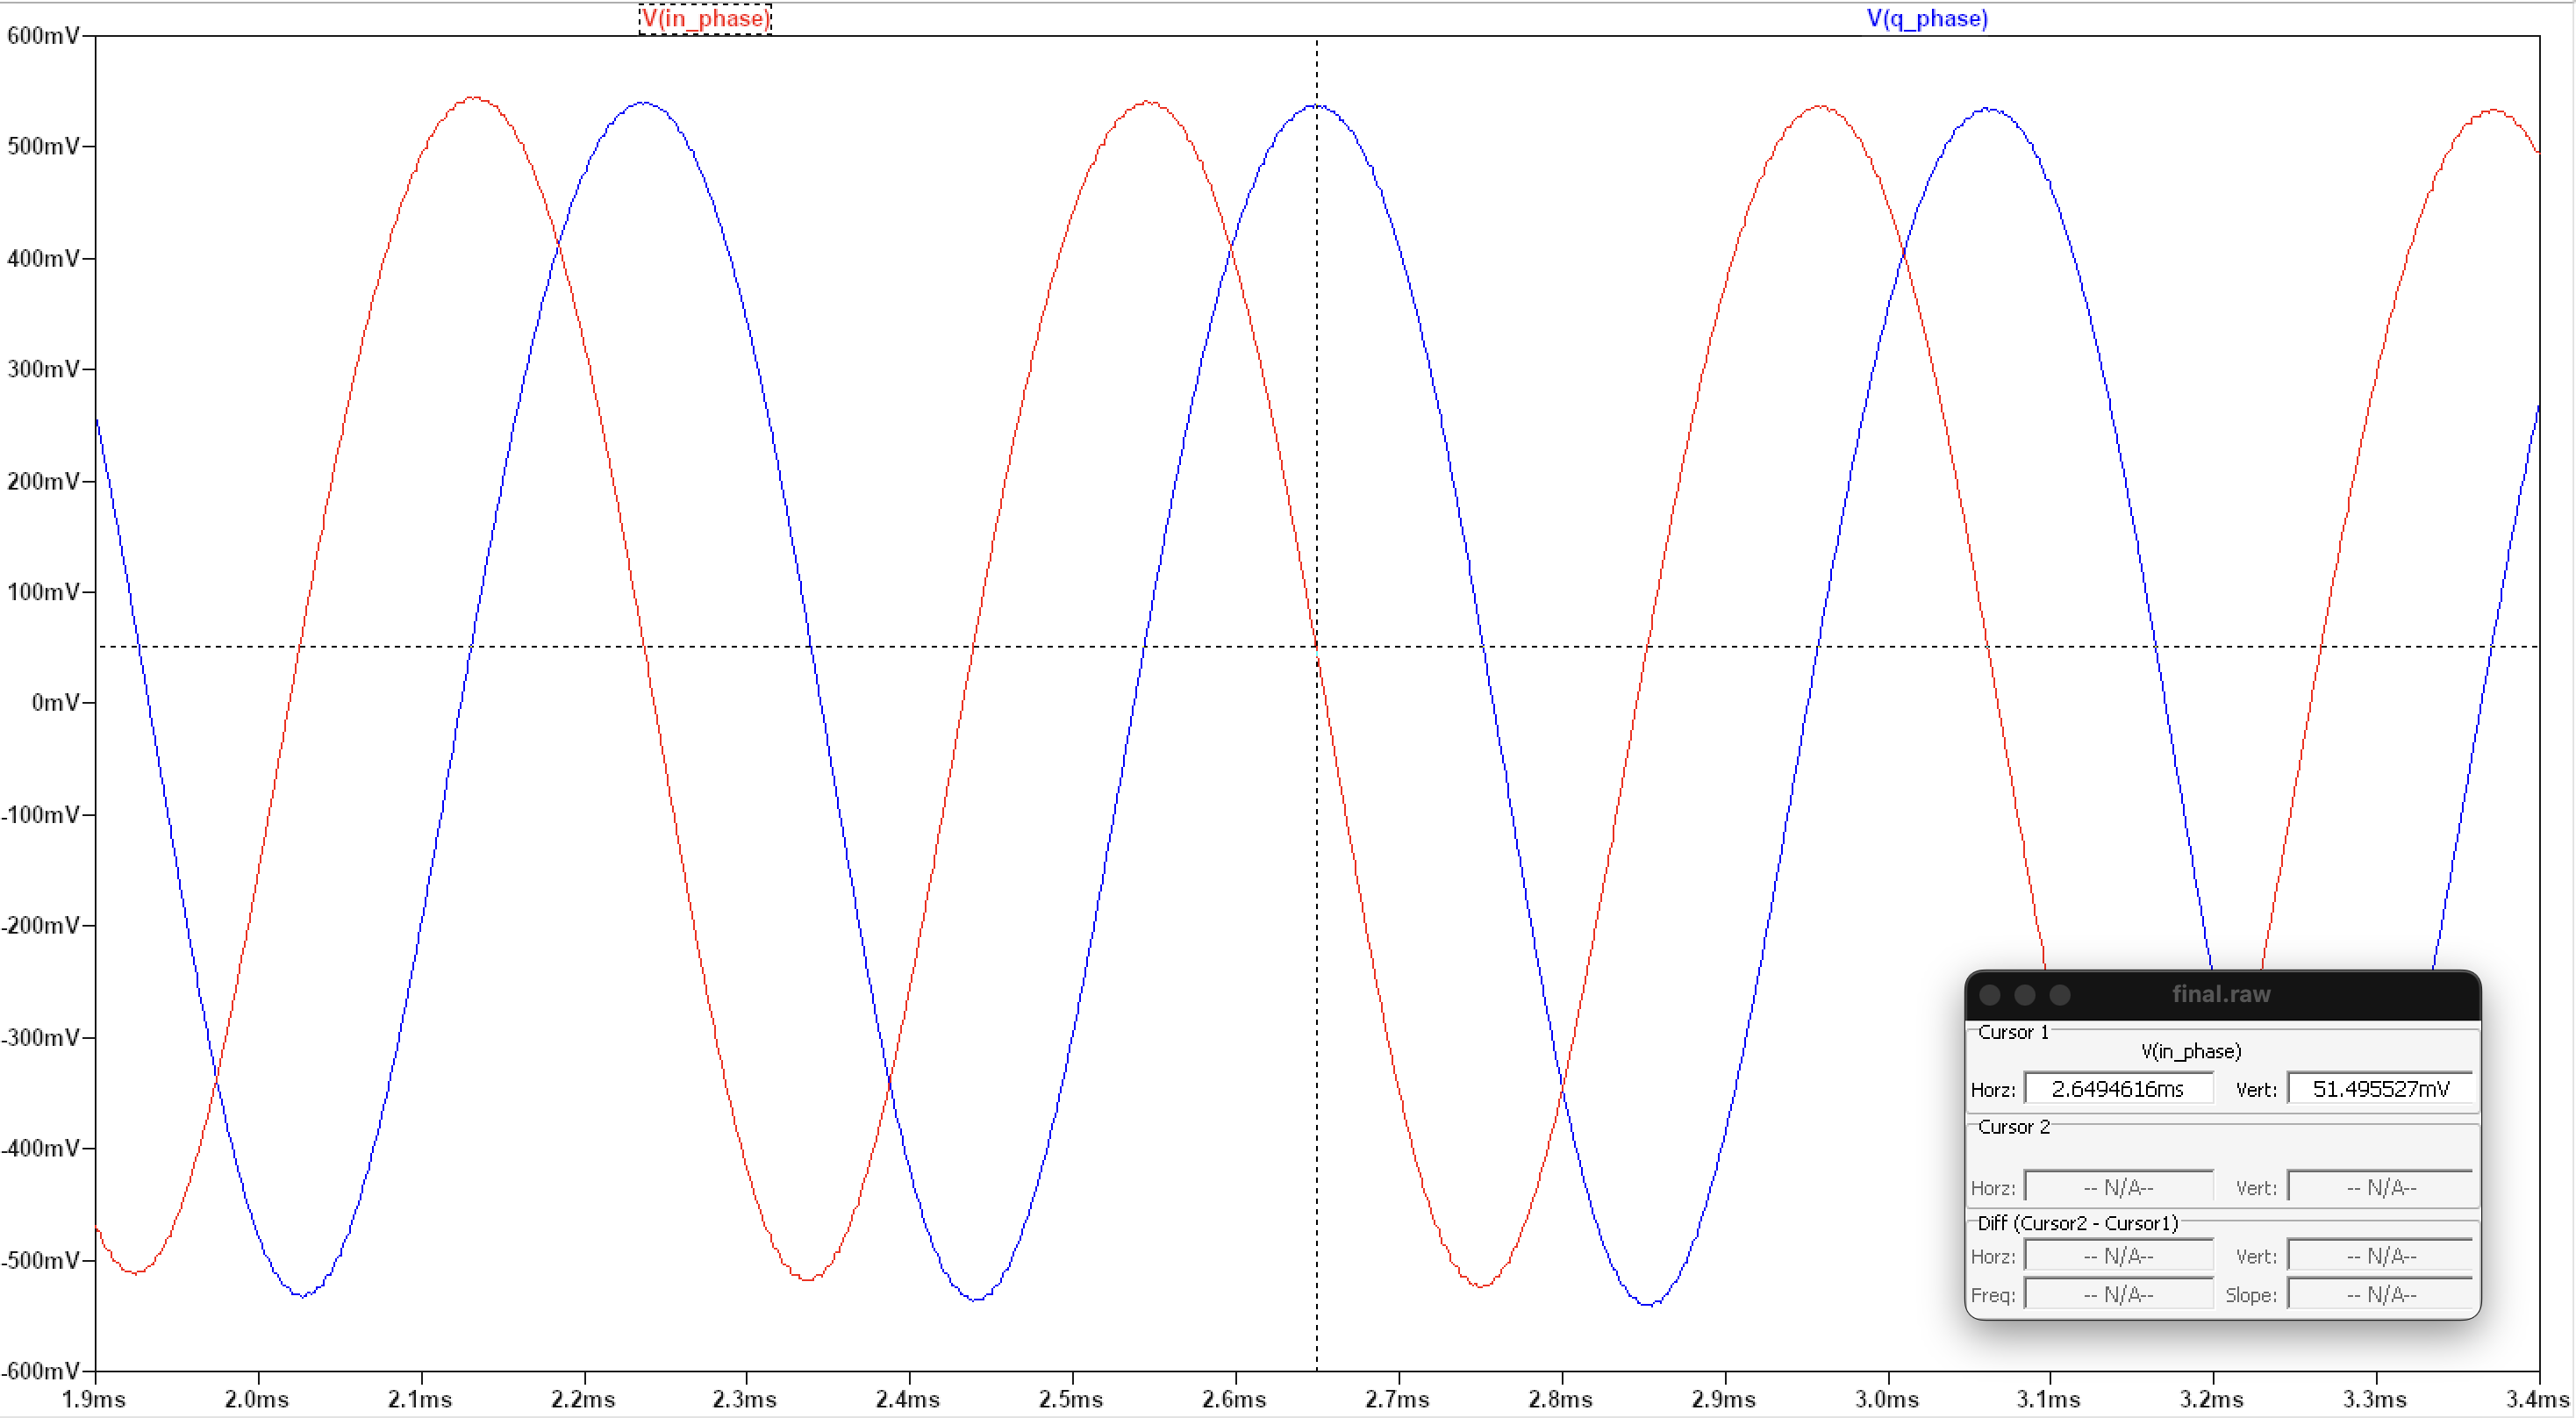
\includegraphics[width=\linewidth]{../report/images/5-phase-diff-iq1.png} \\
      \vspace{0.05cm}
      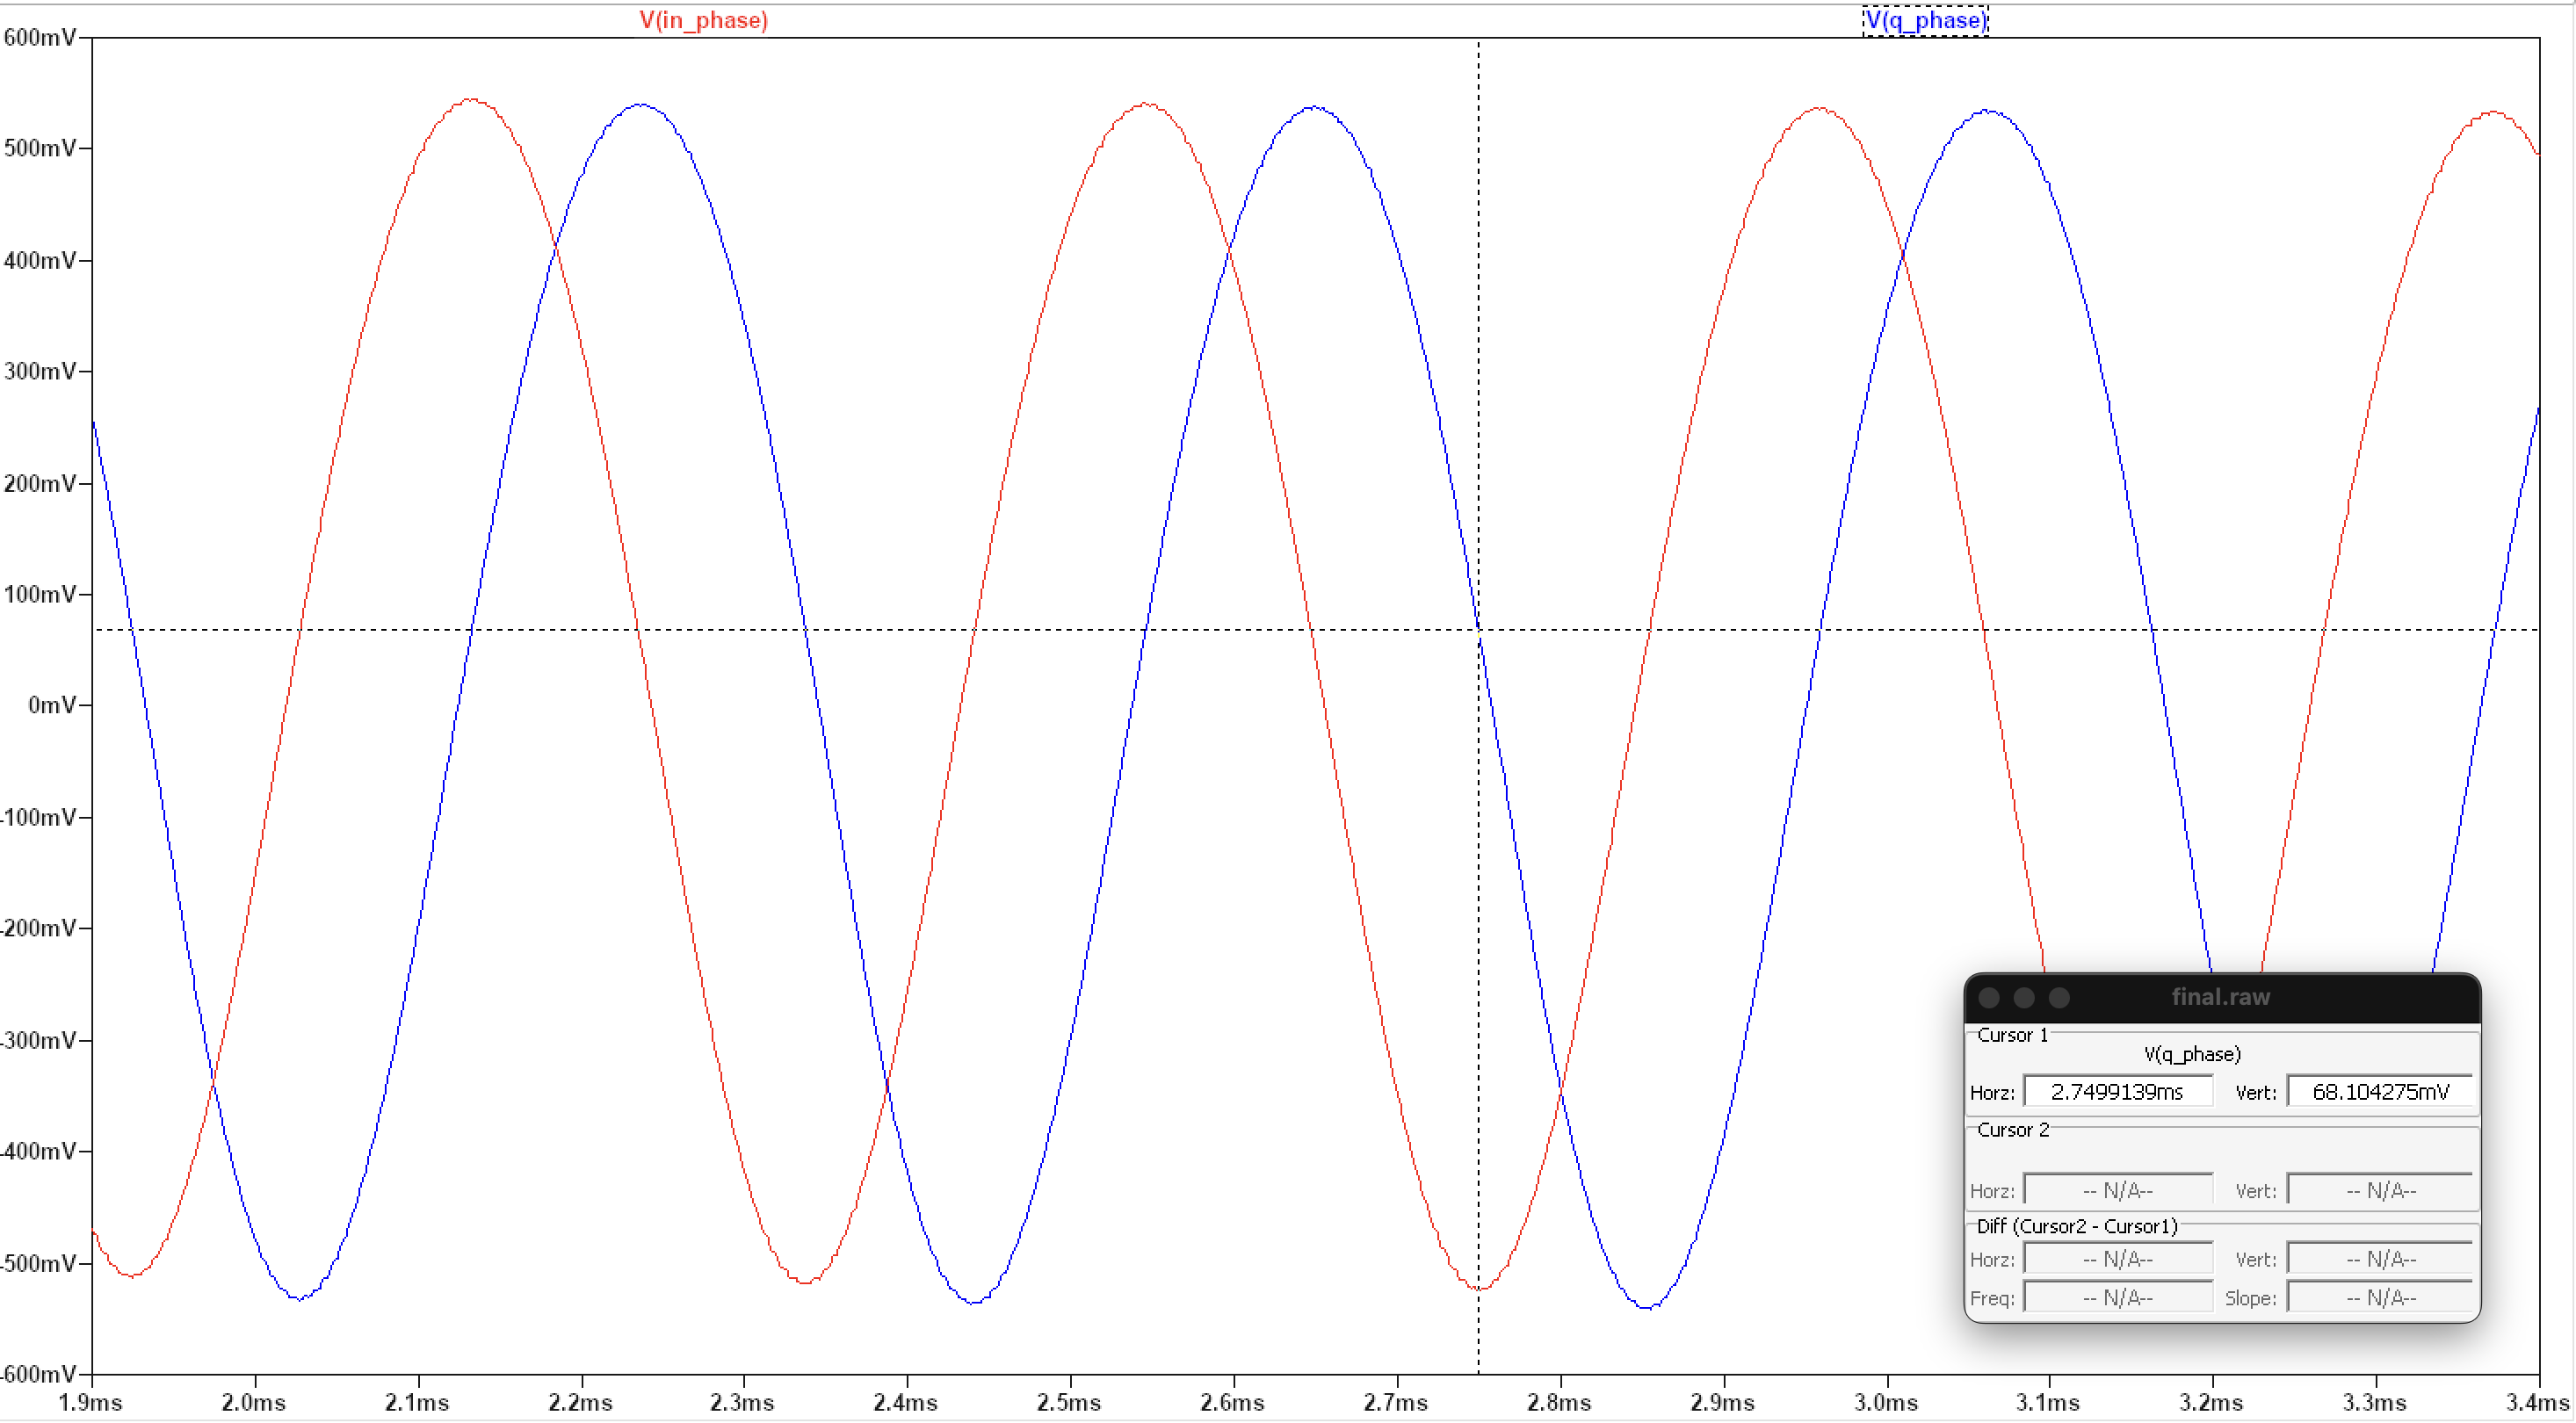
\includegraphics[width=\linewidth]{../report/images/5-phase-diff-iq2.png}
      \vspace{0.05cm}
      \tiny Dual-Channel DSO Phase Difference Captures ($85^\circ - 90^\circ$).
    \end{column}
    \begin{column}{0.5\textwidth}
      \centering
      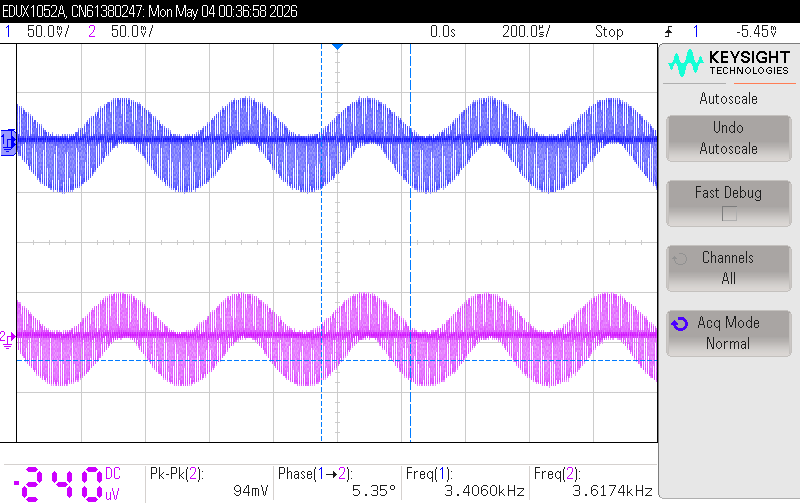
\includegraphics[width=\linewidth]{../report/images/mixer-ouput-both-inphase-and-quadrature-phase.png}
      \vspace{0.1cm}
      \tiny Final DSO Display: Concurrent In-Phase ($I$) and Quadrature ($Q$) IF Outputs.
    \end{column}
  \end{columns}
\end{frame}

% Slide 27: Comprehensive Performance Comparison Table
\begin{frame}{Performance Summary \& Quantitative Comparison}
  \begin{table}
    \centering
    \caption{System Performance Summary: Simulated vs. Measured}
    \resizebox{0.82\linewidth}{!}{%
    \begin{tabular}{|l|c|c|}
      \hline
      \textbf{Parameters} & \textbf{Simulated} & \textbf{Measured} \\
      \hline
      Oscillator Frequency ($f_{\text{osc}}$) & $200\text{ kHz}$ & $174\text{ kHz}$ \\
      \hline
      Oscillator Amplitude (I-phase) & $500\text{ mV}_{\text{peak}}$ & $430\text{ mV}_{\text{peak}}$ \\
      \hline
      Oscillator Amplitude (Q-phase) & $500\text{ mV}_{\text{peak}}$ & $515\text{ mV}_{\text{peak}}$ \\
      \hline
      Input frequency ($f_{\text{in}}$) & $202\text{ kHz}$ & $171\text{ kHz}$ \\
      \hline
      Intermediate Frequency ($f_{\text{IF}}$) & $2\text{ kHz}$ & $3\text{ kHz} - 5\text{ kHz}$ \\
      \hline
      Supply Voltages & $\pm 15\text{ V}$ & $\pm 12\text{ V}$ \\
      \hline
      Mixer Gate Bias ($V_{\text{BIAS}}$) & $1.2\text{ V}$ & $1.2\text{ V}$ \\
      \hline
      Mixer Coupling Cap ($C_C$) & $10\text{ nF}$ & $10\ \mu\text{F}$ \\
      \hline
      Phase Difference (I vs Q) & $93^\circ$ & $85^\circ$ \\
      \hline
      Final IF Amplitude ($V_{\text{IF\_FINAL}}$) & $1.3\text{ V}_{\text{pp}}$ & $800\text{ mV}_{\text{pp}}$ ($\ge 400\text{ mV}_{\text{spec}}$) \\
      \hline
      LPF Components ($R, C$) & $4.7\text{ k}\Omega, 10\text{ nF}$ & $2 \times (2.2\text{ k}\Omega, 10\text{ nF})$ \\
      \hline
    \end{tabular}%
    }
  \end{table}
\end{frame}

\section{Conclusion \& Contributions}

% Slide 28: Summary of Accomplishments & Member Contributions
\begin{frame}{Conclusion \& Group Member Contributions}
  \begin{block}{Project Accomplishments}
    \begin{itemize}
      \item Full implementation and laboratory verification of an analog Quadrature Down Converter operating at $170\text{ kHz}$ with a $5\text{ kHz}$ IF output.
      \item Successfully verified TSMC 180nm CMOS active mixer, 3-op-amp allpass quadrature oscillator, 2-stage cascaded LPF, and discrete CE BJT amplifier stage.
    \end{itemize}
  \end{block}

  \begin{block}{Group Member Contributions}
    \begin{itemize}
      \tiny
      \item \textbf{Katta Sri Kaushik (2025102071):} Quadrature Oscillator design, allpass phase calculations, diode soft limiting network tuning, and LTSpice transient/FFT simulations.
      \item \textbf{Lakshmi Sai Bhargav V (2025102061):} Active NMOS switch mixer design, MOSFET sizing ($W/L, A_S, P_S$), frequency sweep simulations, and integrated system layout.
      \item \textbf{Kushwanth Lanka (2025102072):} Two-stage cascaded RC LPF optimization, CE BJT amplifier design with emitter degeneration for low THD, and physical DSO hardware testing.
    \end{itemize}
  \end{block}
\end{frame}

% Slide 29: Thank You Slide
\begin{frame}
  \centering
  \Huge \textbf{Thank You!} \\
  \vspace{0.5cm}
  \Large Questions \& Technical Discussion
\end{frame}

\end{document}